%  \documentclass[oneside,11pt]{article}

% 
\usepackage{soul}
\usepackage{natbib}
\usepackage{hyperref}
\usepackage{bookmark}
\usepackage{graphicx}             
\graphicspath{{./Figuras/}}

\usepackage{makecell}
\usepackage[margin=1in]{geometry}
\usepackage{float}                
\usepackage{amsmath}
\usepackage{amscd}
\usepackage{amsfonts}
\usepackage{amssymb}
\usepackage{bbm}
\usepackage{booktabs}
\usepackage{nameref}
\usepackage{multirow}
\usepackage[nokeyprefix]{refstyle}
\usepackage{rotating}
\usepackage{threeparttable}
\usepackage{afterpage}
\usepackage{lscape}
\usepackage{enumerate}
\usepackage{caption}
\usepackage{subcaption}
\usepackage{epstopdf}
\usepackage{setspace}
\usepackage{svg}
\usepackage{dsfont}
\usepackage{amsthm}
\usepackage{tocloft}
\usepackage{etoc}
\usepackage{lmodern}
\usepackage{bm}

\epstopdfDeclareGraphicsRule{.tiff}{png}{.png}{convert #1 \OutputFile}
\AppendGraphicsExtensions{.tiff}

\epstopdfDeclareGraphicsRule{.tif}{png}{.png}{convert #1 \OutputFile}
\AppendGraphicsExtensions{.tif}

\usepackage{tikz}
\usetikzlibrary{shapes.geometric, arrows}
\usetikzlibrary{calc}
\usetikzlibrary{matrix}

\tikzset{ 
    table/.style={
        matrix of nodes,
        row sep=-\pgflinewidth,
        column sep=-\pgflinewidth,
        nodes={
            rectangle,
            draw=black,
            align=center
        },
        minimum height=1.5em,
        text depth=0.5ex,
        text height=2ex,
        nodes in empty cells,
%%
        every even row/.style={
            nodes={fill=gray!20}
        },
        column 1/.style={
            nodes={text width=2em,font=\bfseries}
        },
        row 1/.style={
            nodes={
                fill=black,
                text=white,
                font=\bfseries
            }
        }
    }
}


\usepackage{colortbl}

\newtheorem{theorem}{Theorem}
\newtheorem{claim}[theorem]{Claim}
\newtheorem{prop}[theorem]{Proposition} 
\newtheorem{cor}[theorem]{Corollary} 

\DeclareRobustCommand{\hlgr}[1]{{\sethlcolor{green}\hl{#1}}}


\usepackage{comment}
%para esconder columnas en tablas (enrique)
\usepackage{array}
\newcolumntype{H}{>{\setbox0=\hbox\bgroup}c<{\egroup}@{}}
\linespread{1.25}

\newcommand{\wh}{\widehat}
\usepackage{anyfontsize}

\usepackage[linesnumbered,vlined,ruled,commentsnumbered]{algorithm2e}

\DontPrintSemicolon
\newcommand{\To}{\mbox{\upshape\bfseries to}}
% %%% HELPER CODE FOR DEALING WITH EXTERNAL REFERENCES
% \usepackage{xr}
% \makeatletter
% \newcommand*{\addFileDependency}[1]{
%   \typeout{(#1)}
%   \@addtofilelist{#1}
%   \IfFileExists{#1}{}{\typeout{No file #1.}}
% }
% \makeatother


% \newcommand*{\myexternaldocument}[1]{
%     \externaldocument{#1}
%     \addFileDependency{#1.tex}
%     \addFileDependency{#1.aux}
% }

% %\myexternaldocument{OA}

% %%%%%%%%%%%%%%%%%%%%%%%%%%%%%%%% DOCUMENT
% \begin{document}

%%%%%%%%%%%%%%%%%%%%%%%%%%%%%%%%%%%%%%%%%%%%%%%

% APPENDIX 
\setcounter{table}{0}
\setcounter{figure}{0}
\setcounter{section}{0}
\pagenumbering{gobble}


\begin{center}
	\LARGE The limits of self-commitment and private paternalism \\[0.5em]
	\Large{Appendix $-$ For Online Publication} \\[1em]
	\large \author{Craig McIntosh \and Isaac Meza \and Joyce Sadka \and Enrique Seira}
\end{center}

\appendix
\pagenumbering{arabic}
\renewcommand\thefigure{OA-\arabic{figure}}
\renewcommand\thetable{OA-\arabic{table}}
\renewcommand*{\thepage}{OA - \arabic{page}}
\renewcommand\thesection{Appendix \Alph{section}.}
\renewcommand\thesubsection{\Alph{section}.\arabic{subsection}}

%\renewcommand{\cftparskip}{0em} % NOT NEEDED
\renewcommand\cftsecdotsep{\cftdotsep}
\renewcommand\cftsubsecdotsep{\cftnodots}
\renewcommand{\cftsecnumwidth}{6em}
 \renewcommand{\cftpnumalign}{r}
%\renewcommand{\cftsecleader}{\normalfont\cftdotfill{\cftsecdotsep}}


\renewcommand{\cftsecleader}{\cftdotfill{\cftsecdotsep}\hspace{1.8em}}
%\renewcommand{\cftsecpagefont}{20em}
%\renewcommand{\cftfignumwidth}{6em}
%\renewcommand{\cfttabnumwidth}{3.3em}

%\tableofcontents
\etocdepthtag.toc{mtappendix}
\etocsettagdepth{mtchapter}{none}
\etocsettagdepth{mtappendix}{subsection}

\setstretch{0.9}
%\renewcommand\contentsname{} % the empty name

\begingroup
\let\clearpage\relax
%\vspace{-1.5em} % the removed space. Set as appropriate
\tableofcontents
\endgroup


\newpage



\section{ Further results}
\vspace{.2in}


\begin{table}[H]
\caption{Number of pawns balance before and after the experiment}
\label{num_pawns_bal}
\begin{center}
\scriptsize{% Table generated by Excel2LaTeX from sheet 'num_pawns_bal'
\begin{tabular}{lcccc}
\toprule
      & \multicolumn{4}{c}{Pawns per day} \\
\midrule
      & 0-degree & 1-degree & 2-degree & 3-degree \\
\midrule
\midrule
      & (1)   & (2)   & (3)   & (4) \\
\midrule
\midrule
$\beta_a$ & 2.48  & -3.32 & -0.65 & -0.65 \\
      & (1.36) & (1.85) & (2.80) & (2.80) \\
$\beta_b$ & 0.20  & 1.82  & 1.32  & 1.32 \\
      & (0.97) & (0.93) & (0.67) & (0.67) \\
      &       &       &       &  \\
\midrule
Observations & 628   & 628   & 628   & 628 \\
R-sq  & 0.737 & 0.747 & 0.747 & 0.747 \\
Branch FE & \checkmark & \checkmark & \checkmark & \checkmark \\
\bottomrule
\bottomrule
\end{tabular}%
}
\end{center}
 \scriptsize 
%\textit{Do file: } \texttt{num\_pawns\_bal.do}
\end{table}

\subsection{Some materials}

\vspace{.1in}

\subsection{Pictures}

\begin{figure}[H]
     \caption{Some Pawnshops}
    \label{PawnshopPicture}
    \begin{center}
    \begin{subfigure}{0.42\textwidth}
    \caption{Appraiser/tellers inside a pawnshop}
        \centering
        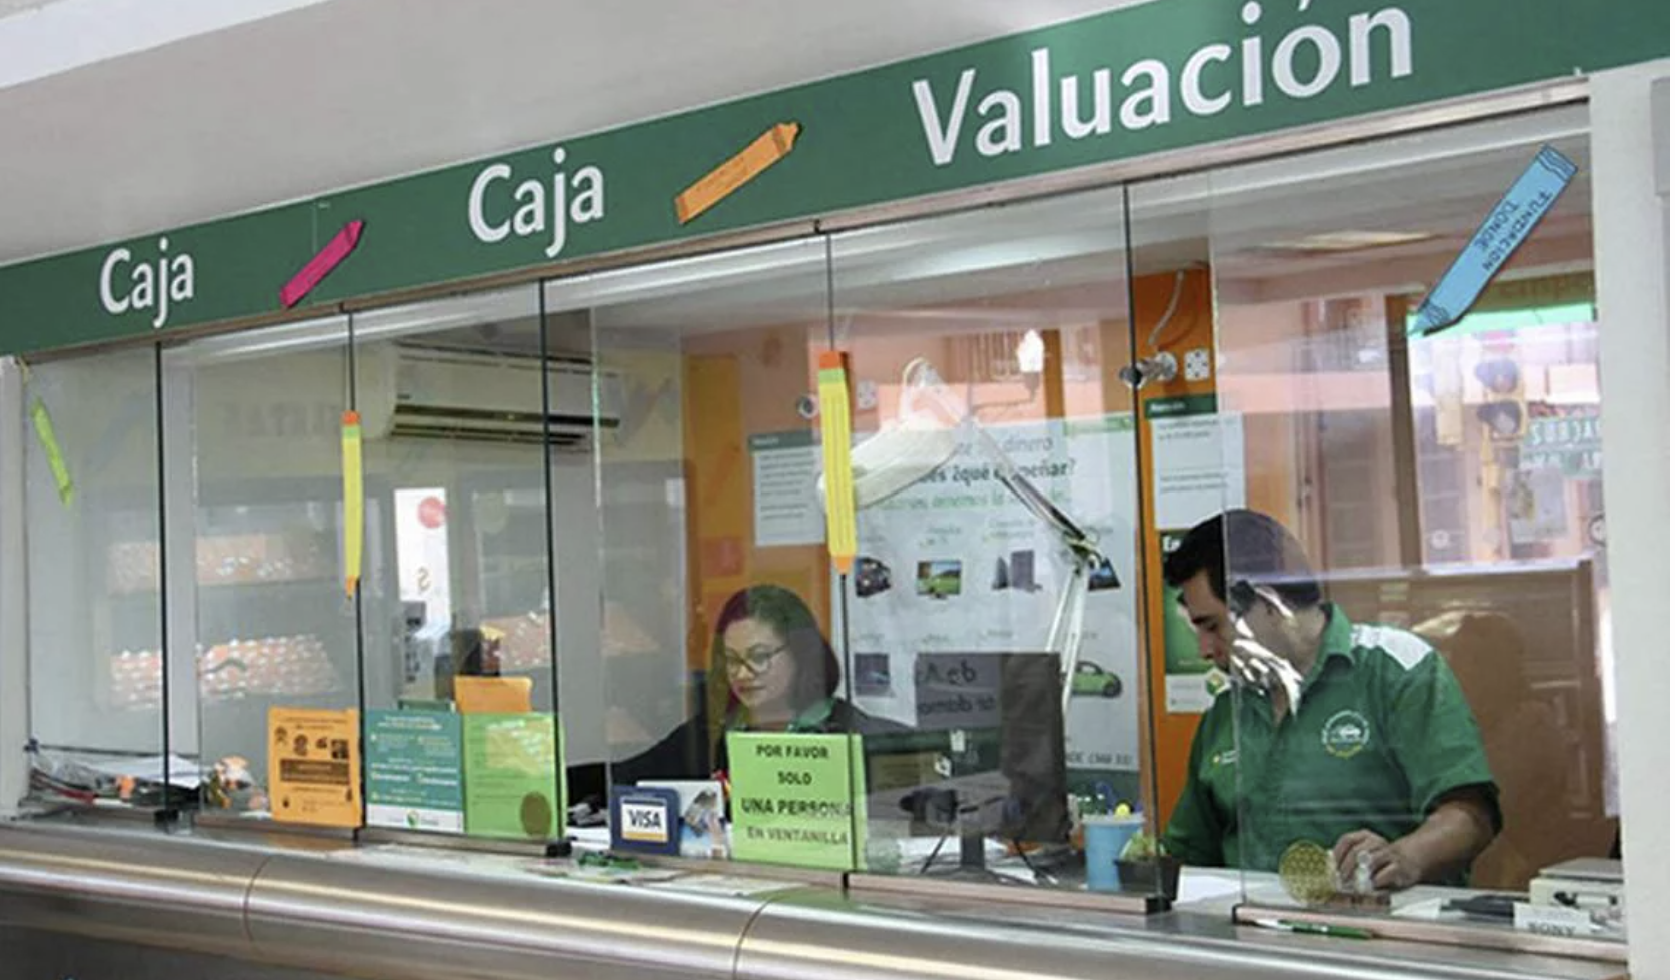
\includegraphics[width=\textwidth]{Figuras/empenio9.png}
    \end{subfigure}
        \begin{subfigure}{0.45\textwidth}
    \caption{Pawnshop}
        \centering
        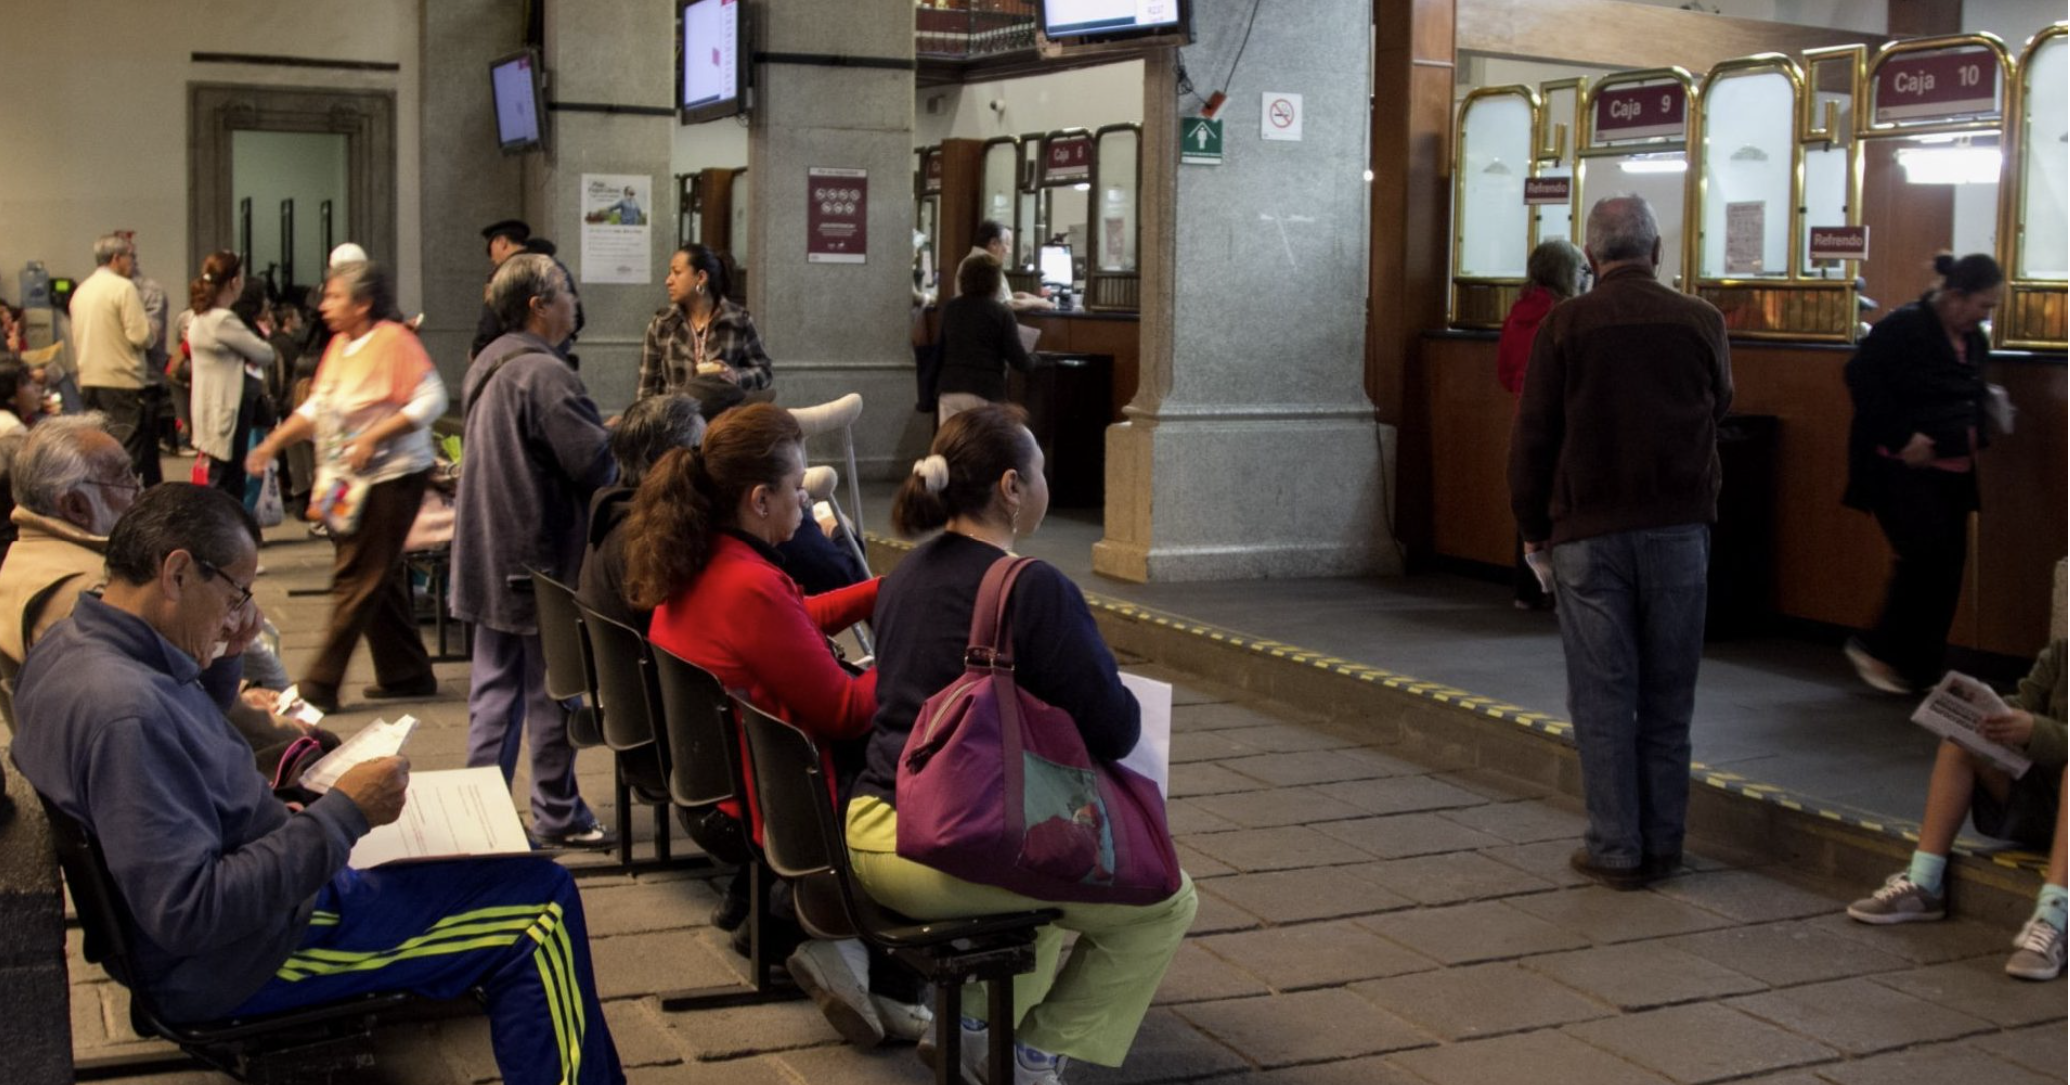
\includegraphics[width=\textwidth]{Figuras/empenio11.png}
    \end{subfigure}
    
        \vspace{3ex}

    \begin{subfigure}{0.45\textwidth}
    \caption{Pawnshop}
        \centering
        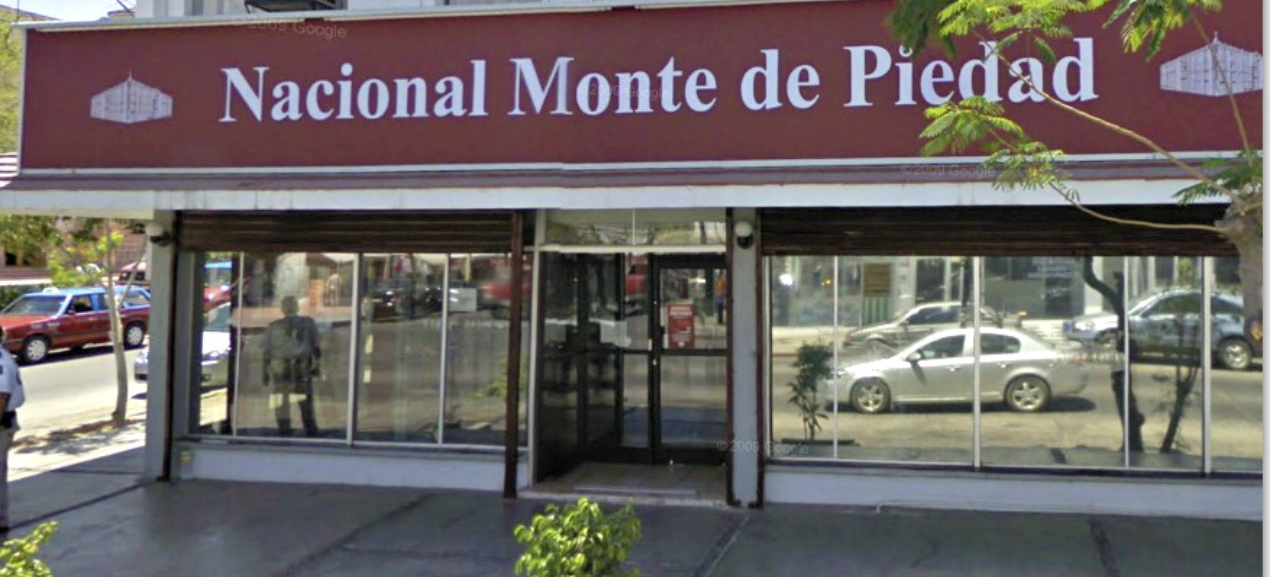
\includegraphics[width=\textwidth]{Figuras/empenio2.png}
    \end{subfigure}
    \begin{subfigure}{0.42\textwidth}
    \caption{Lost pawns which are for sale}
        \centering
        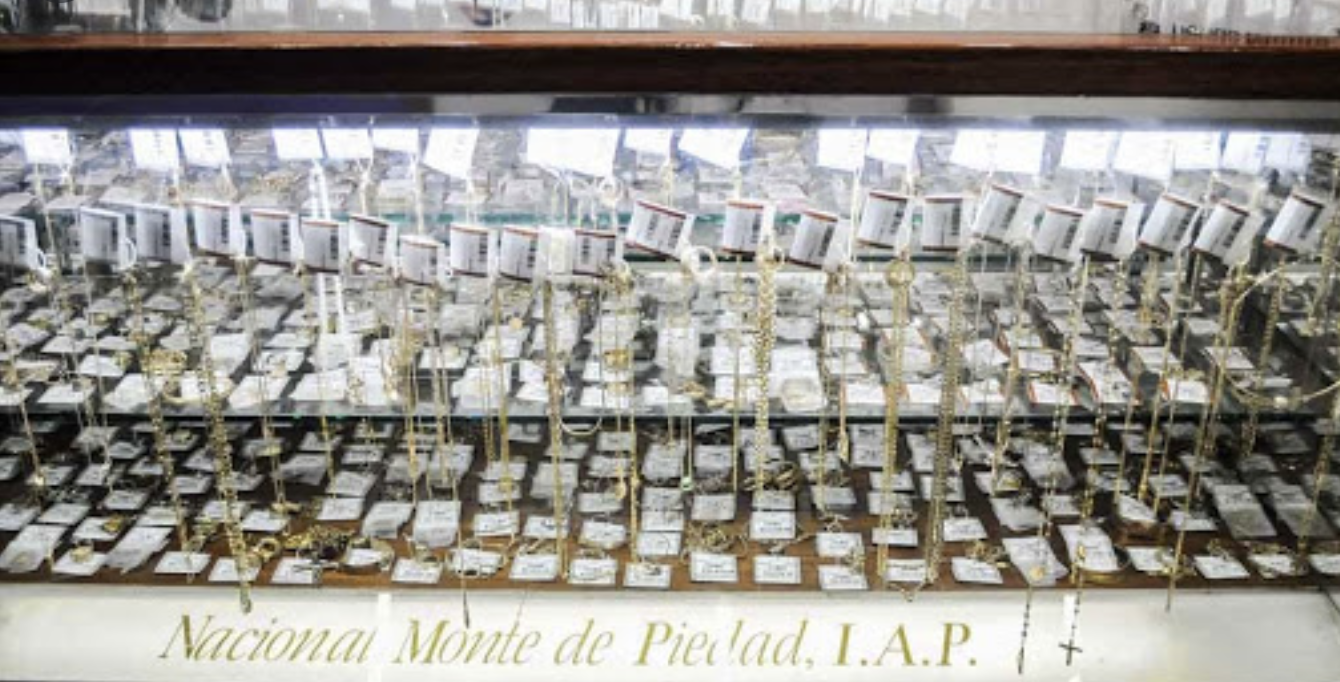
\includegraphics[width=\textwidth]{Figuras/empenio3.png}
    \end{subfigure}
       

    
    \end{center}
    \scriptsize
        This figure  shows pictures of pawnshops in Mexico city. They do not necessarily coincide with Lender P for confidentiality. 
\end{figure}



\vspace{.1in}
\begin{figure}[H]
     \caption{Gold buyers next to pawnshops}
    \label{GoldBuyers}
    \begin{center}
    \begin{subfigure}{.49\textwidth}
    \caption{Gold buyer next to pawnshop 1}
        \centering
        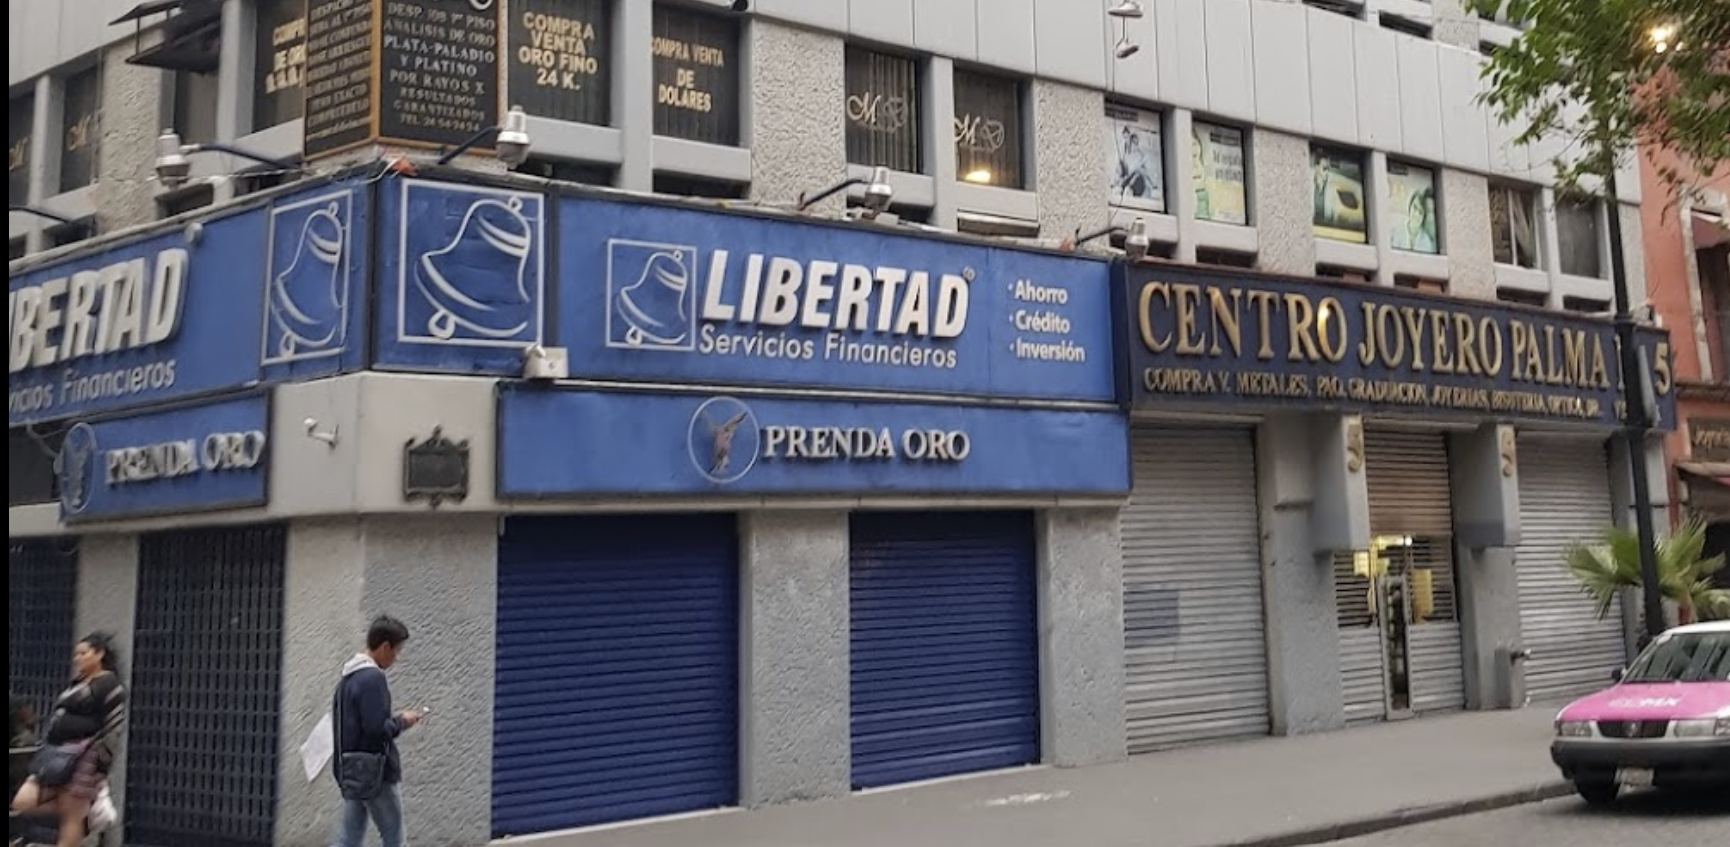
\includegraphics[width=\textwidth]{Figuras/empenio7.png}
    \end{subfigure}
    \begin{subfigure}{.49\textwidth}
    \caption{Gold buyer next to pawnshop 1}
        \centering
        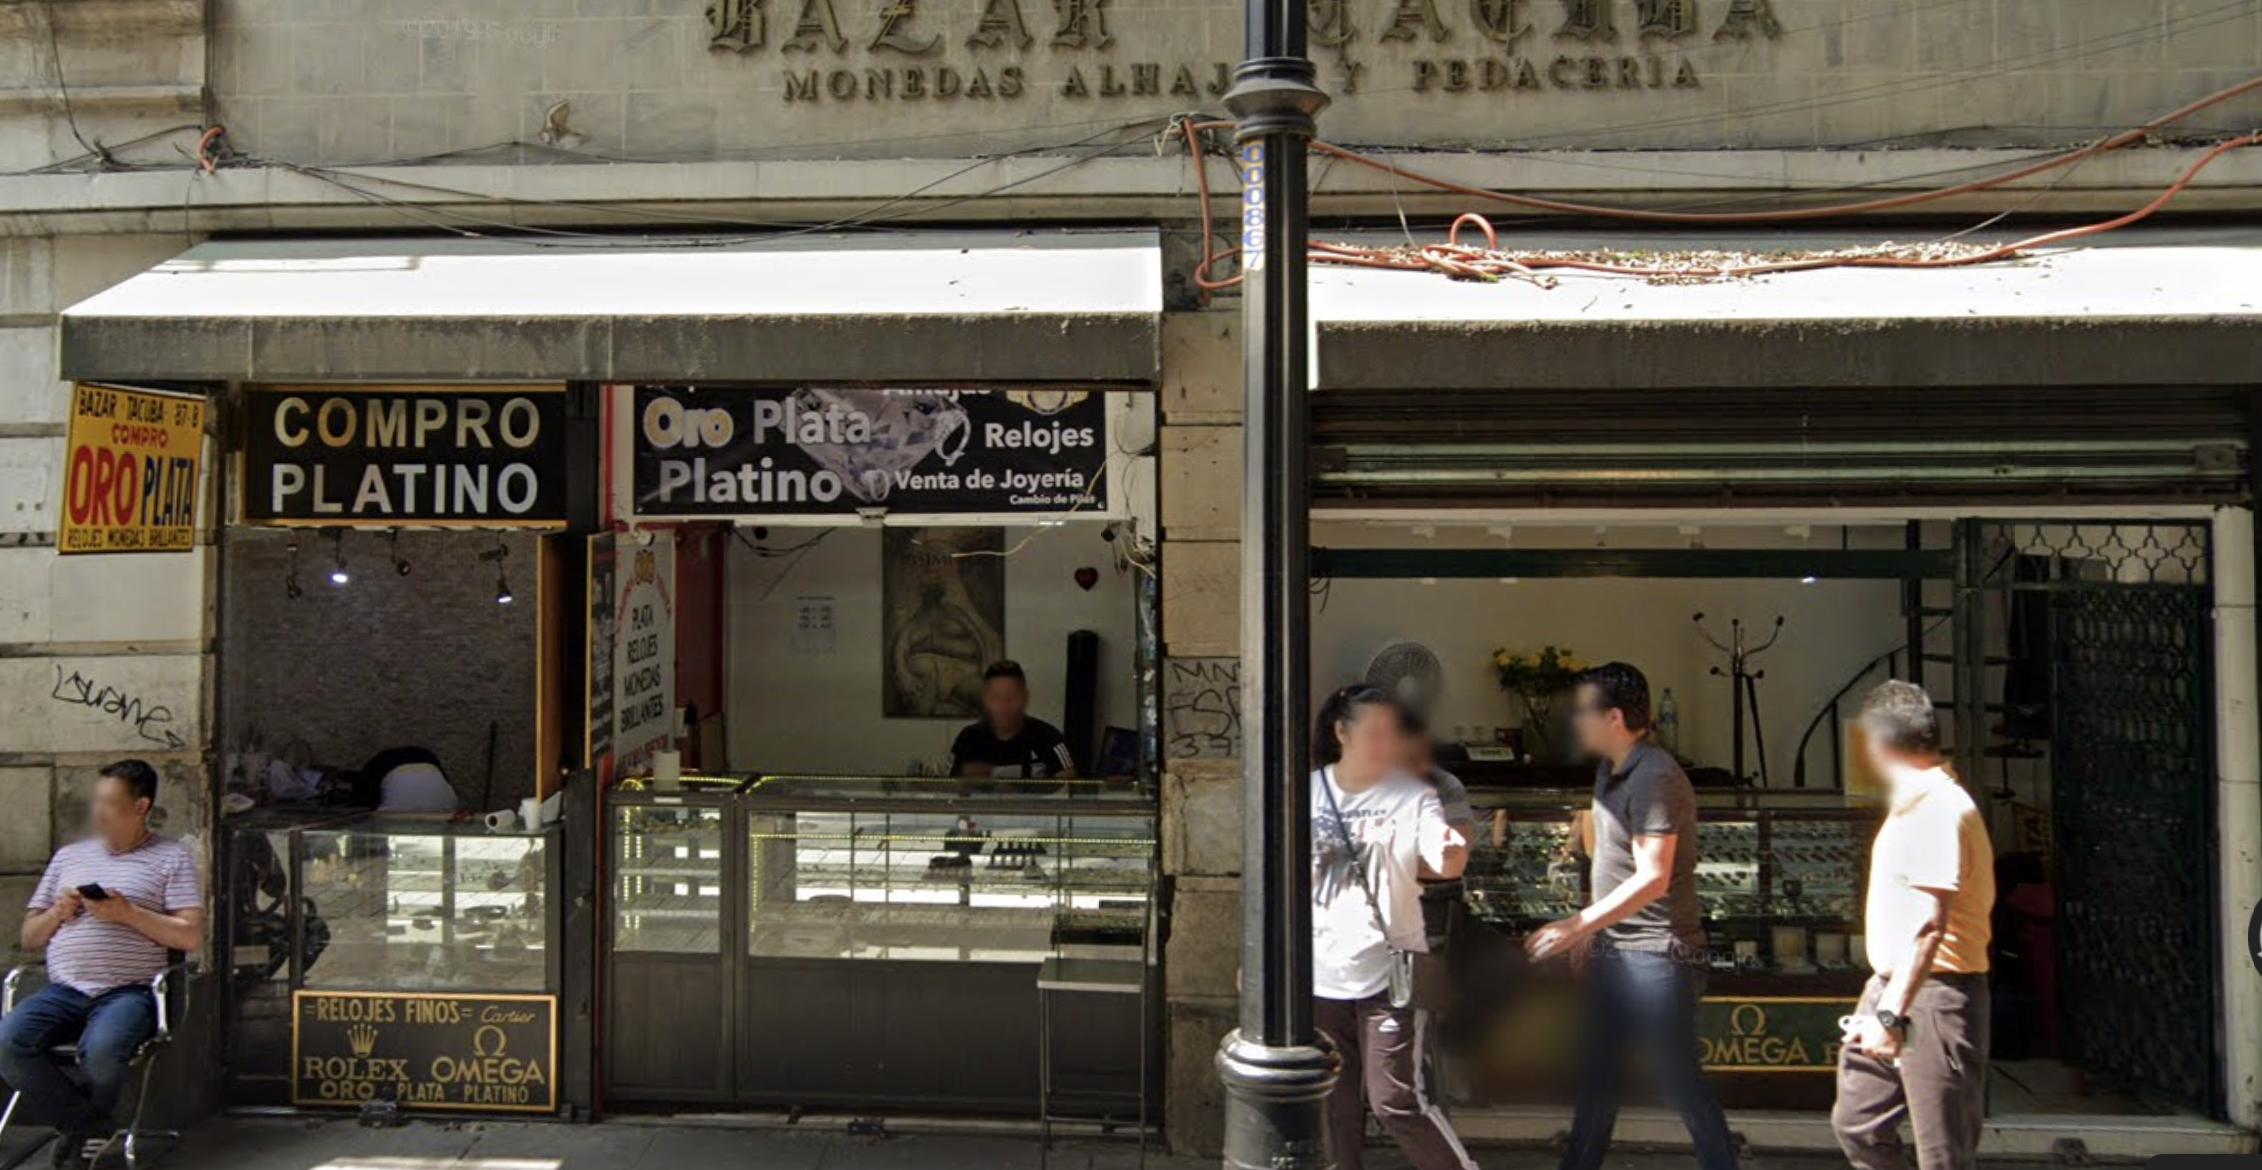
\includegraphics[width=\textwidth]{Figuras/empenio8.png}
    \end{subfigure}
       \vspace{3ex}
       
    \end{center}
    \scriptsize
        This figure shows pictures of gold buyers next to pawnshops in Mexico city. They do not necessarily coincide with Lender P for confidentiality. 
\end{figure}




%\begin{figure}[H]
%        \caption{Booklet with product information}
%    \label{micas}
%    \begin{center}
%        \centering
%        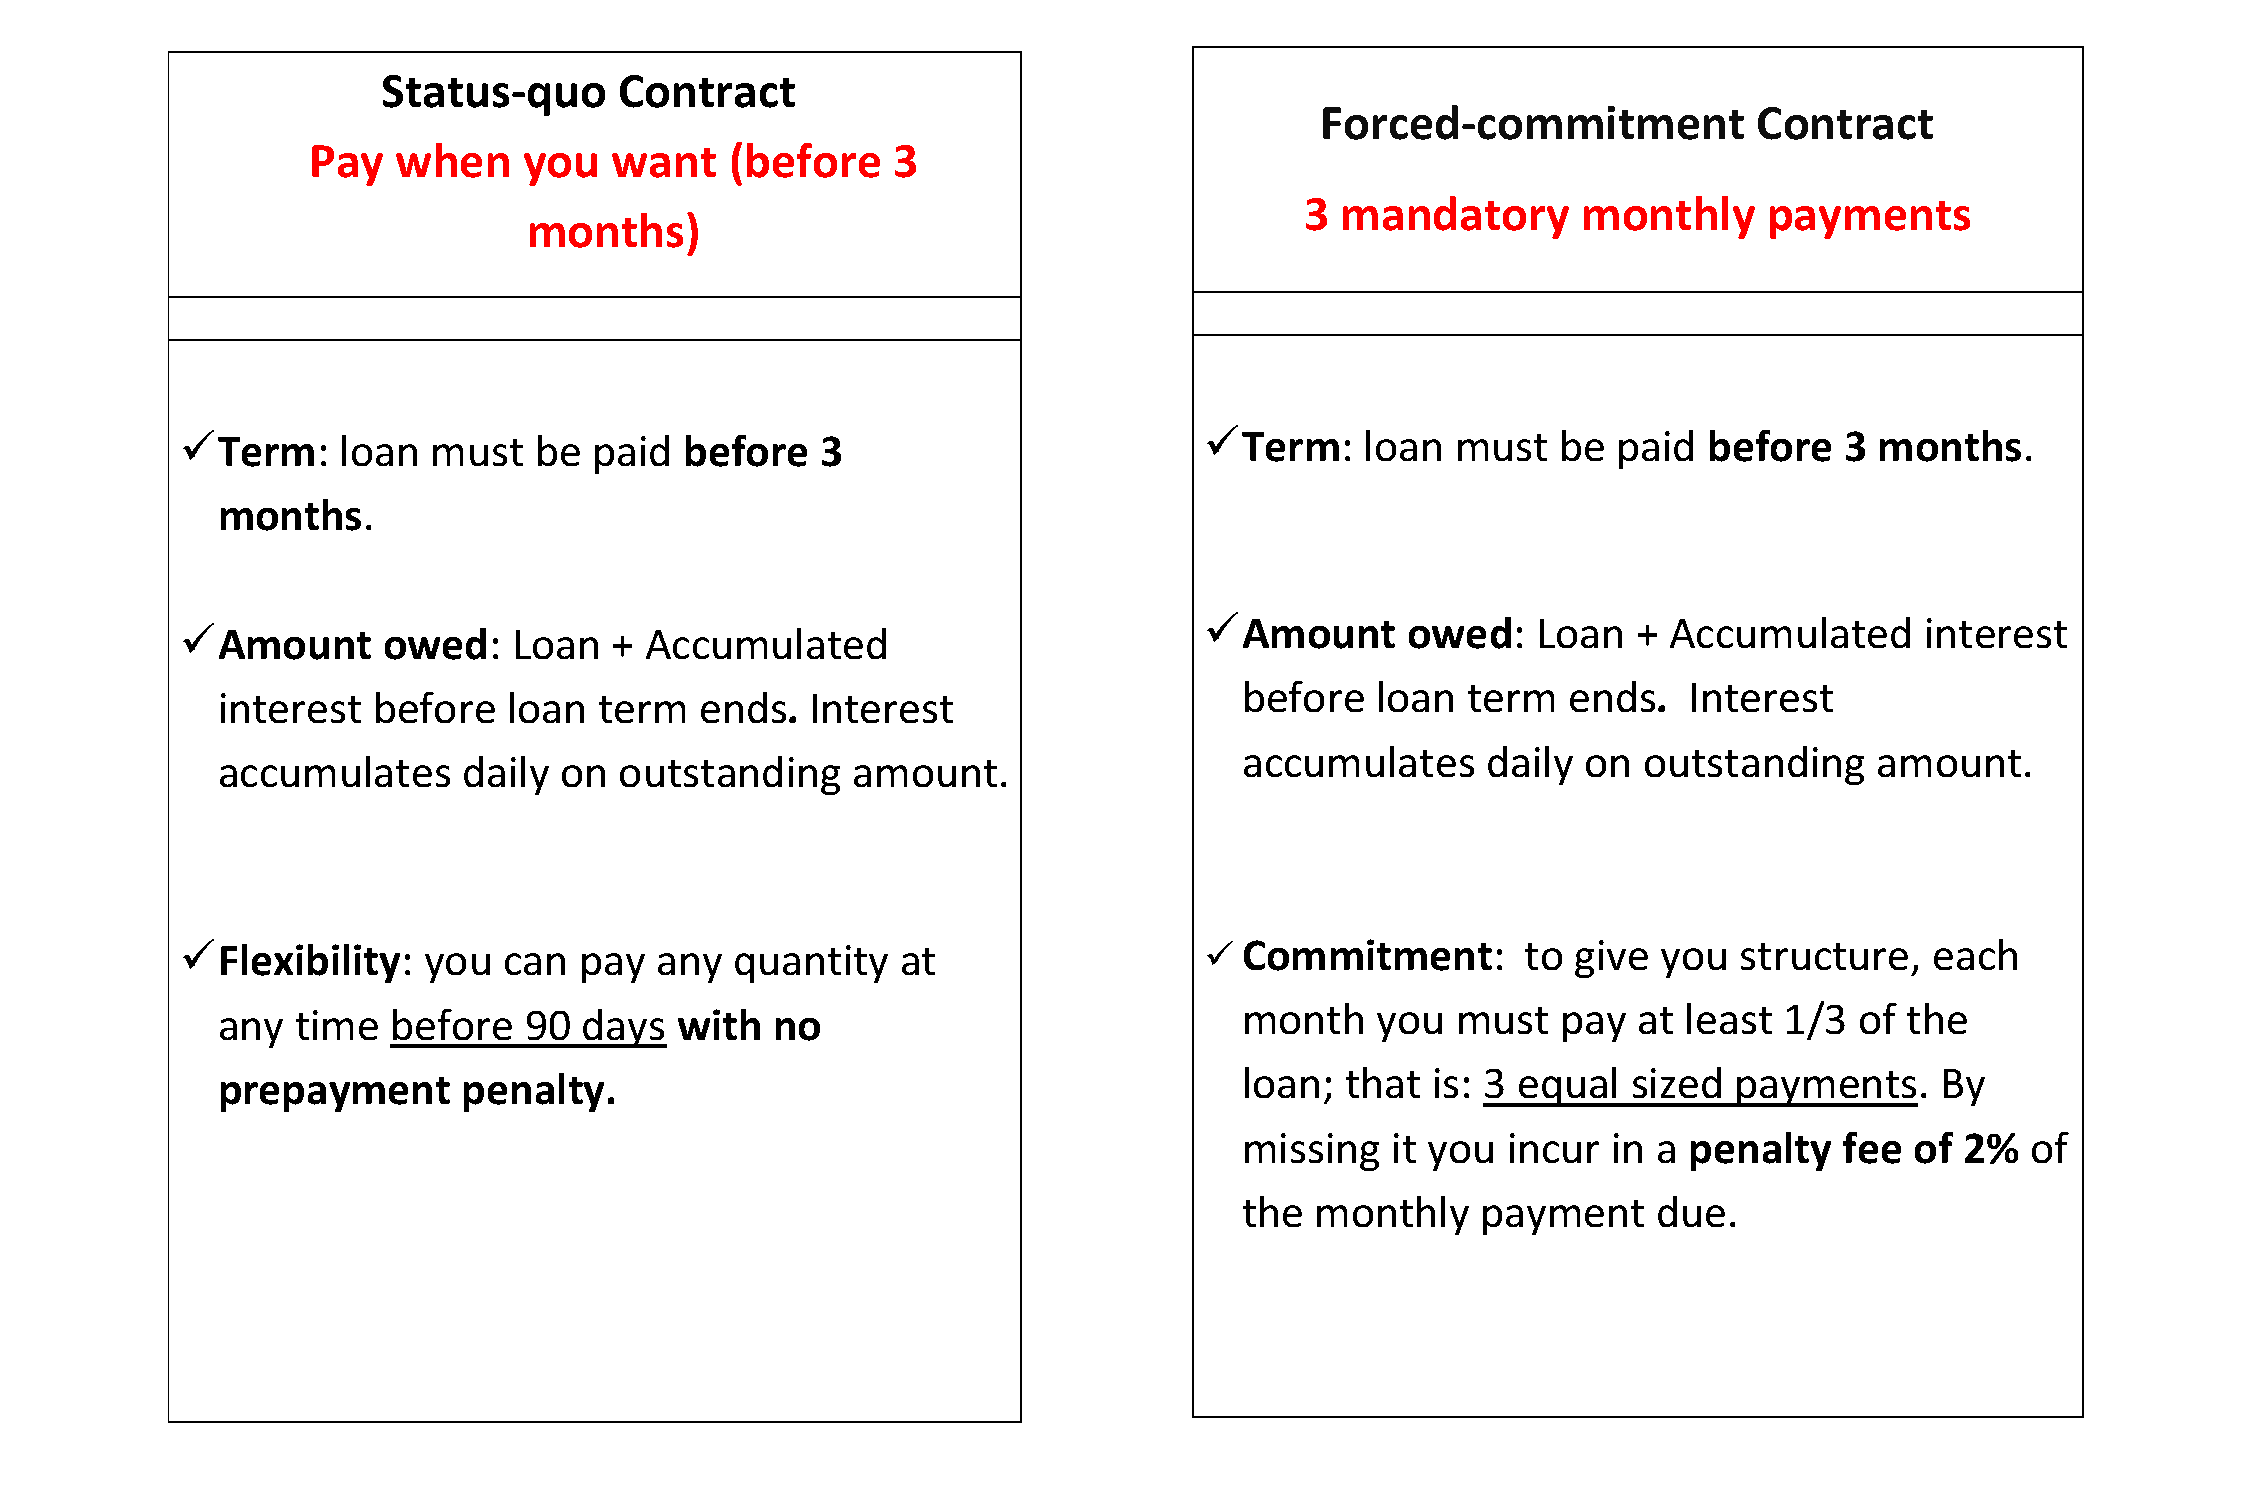
\includegraphics[width=\textwidth]{micas.pdf}
%    \end{center}
%     \footnotesize \textit{Notes: } 
%      \footnotesize{ }
%\end{figure}


%\begin{figure}[H]
%     \caption{Booklet with product information translated}
%    \label{booklet_translate2}
%    \begin{center}
%    \begin{subfigure}{.9\textwidth}
%        \centering
%        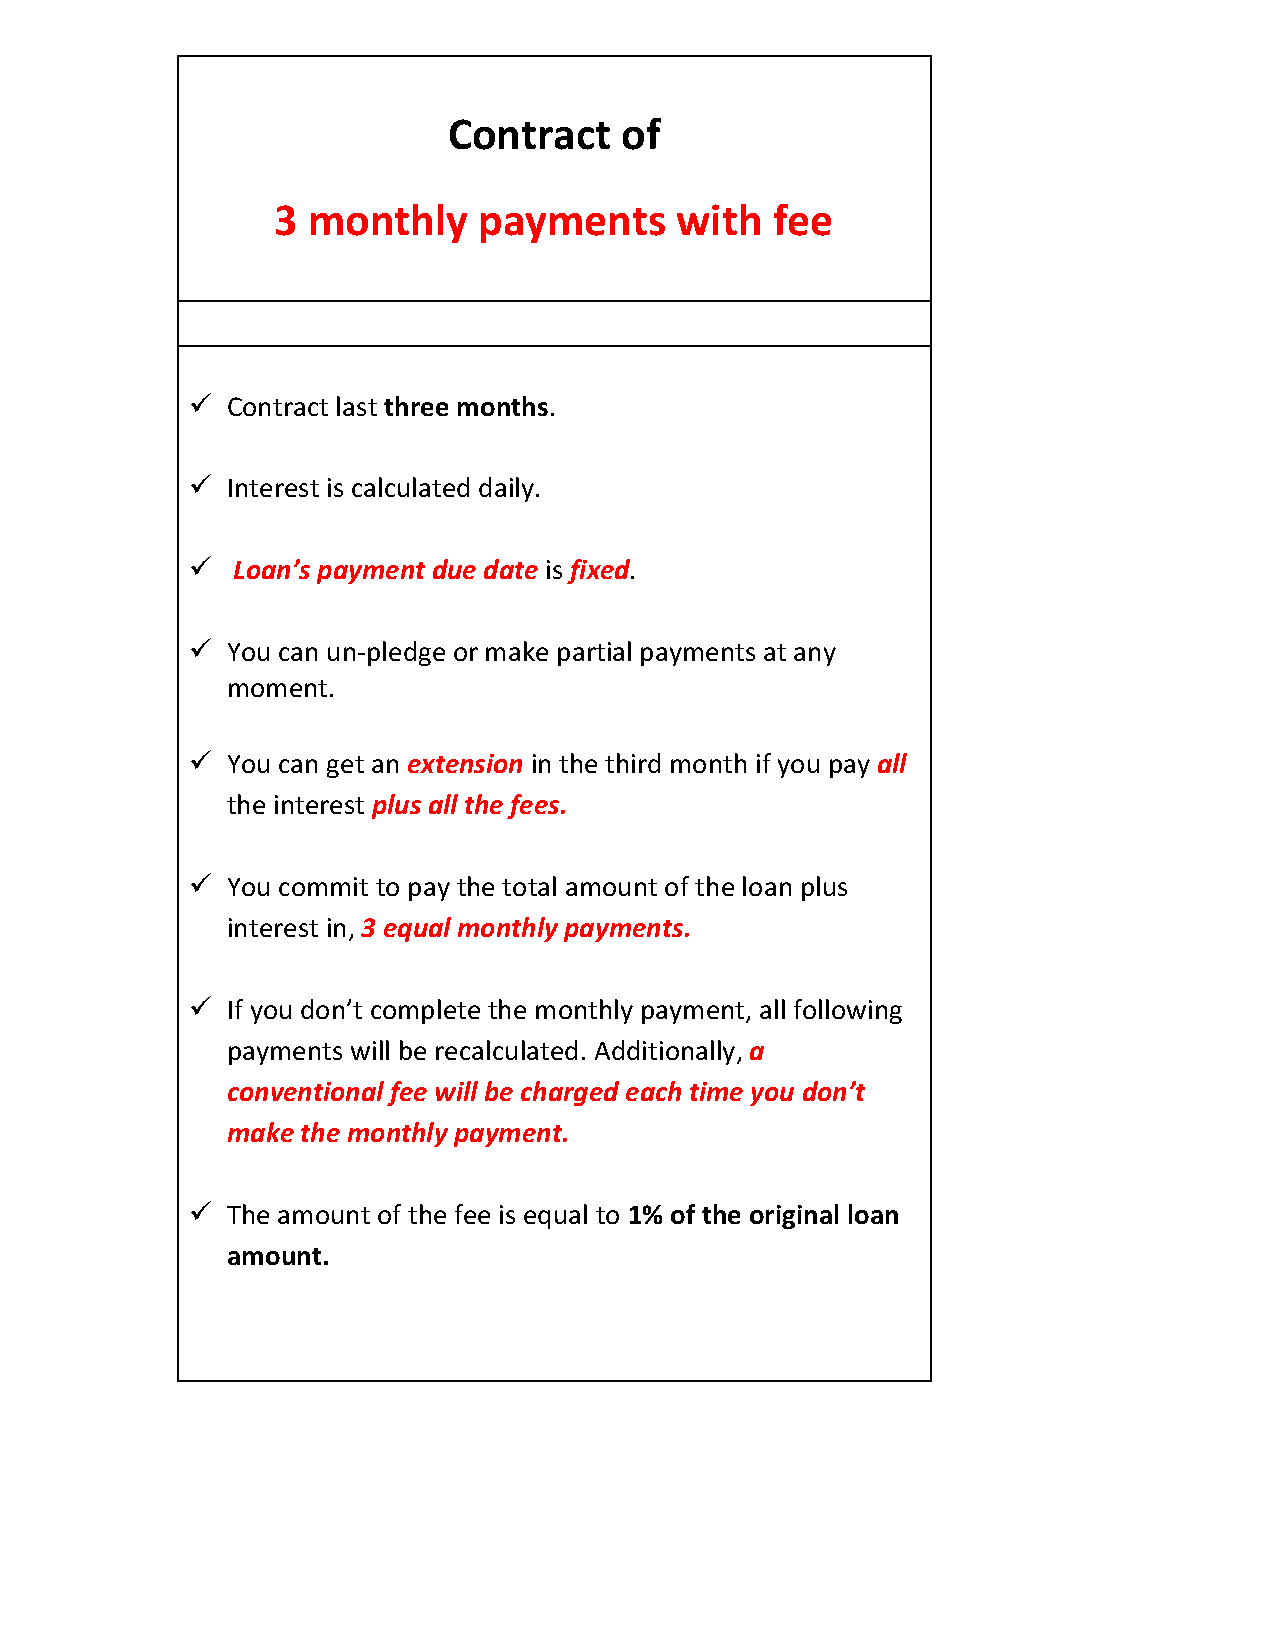
\includegraphics[width=\textwidth]{Figuras/MP_F.pdf}
%    \end{subfigure}
    %\begin{subfigure}{0.55\textwidth}
    %   \centering
    %  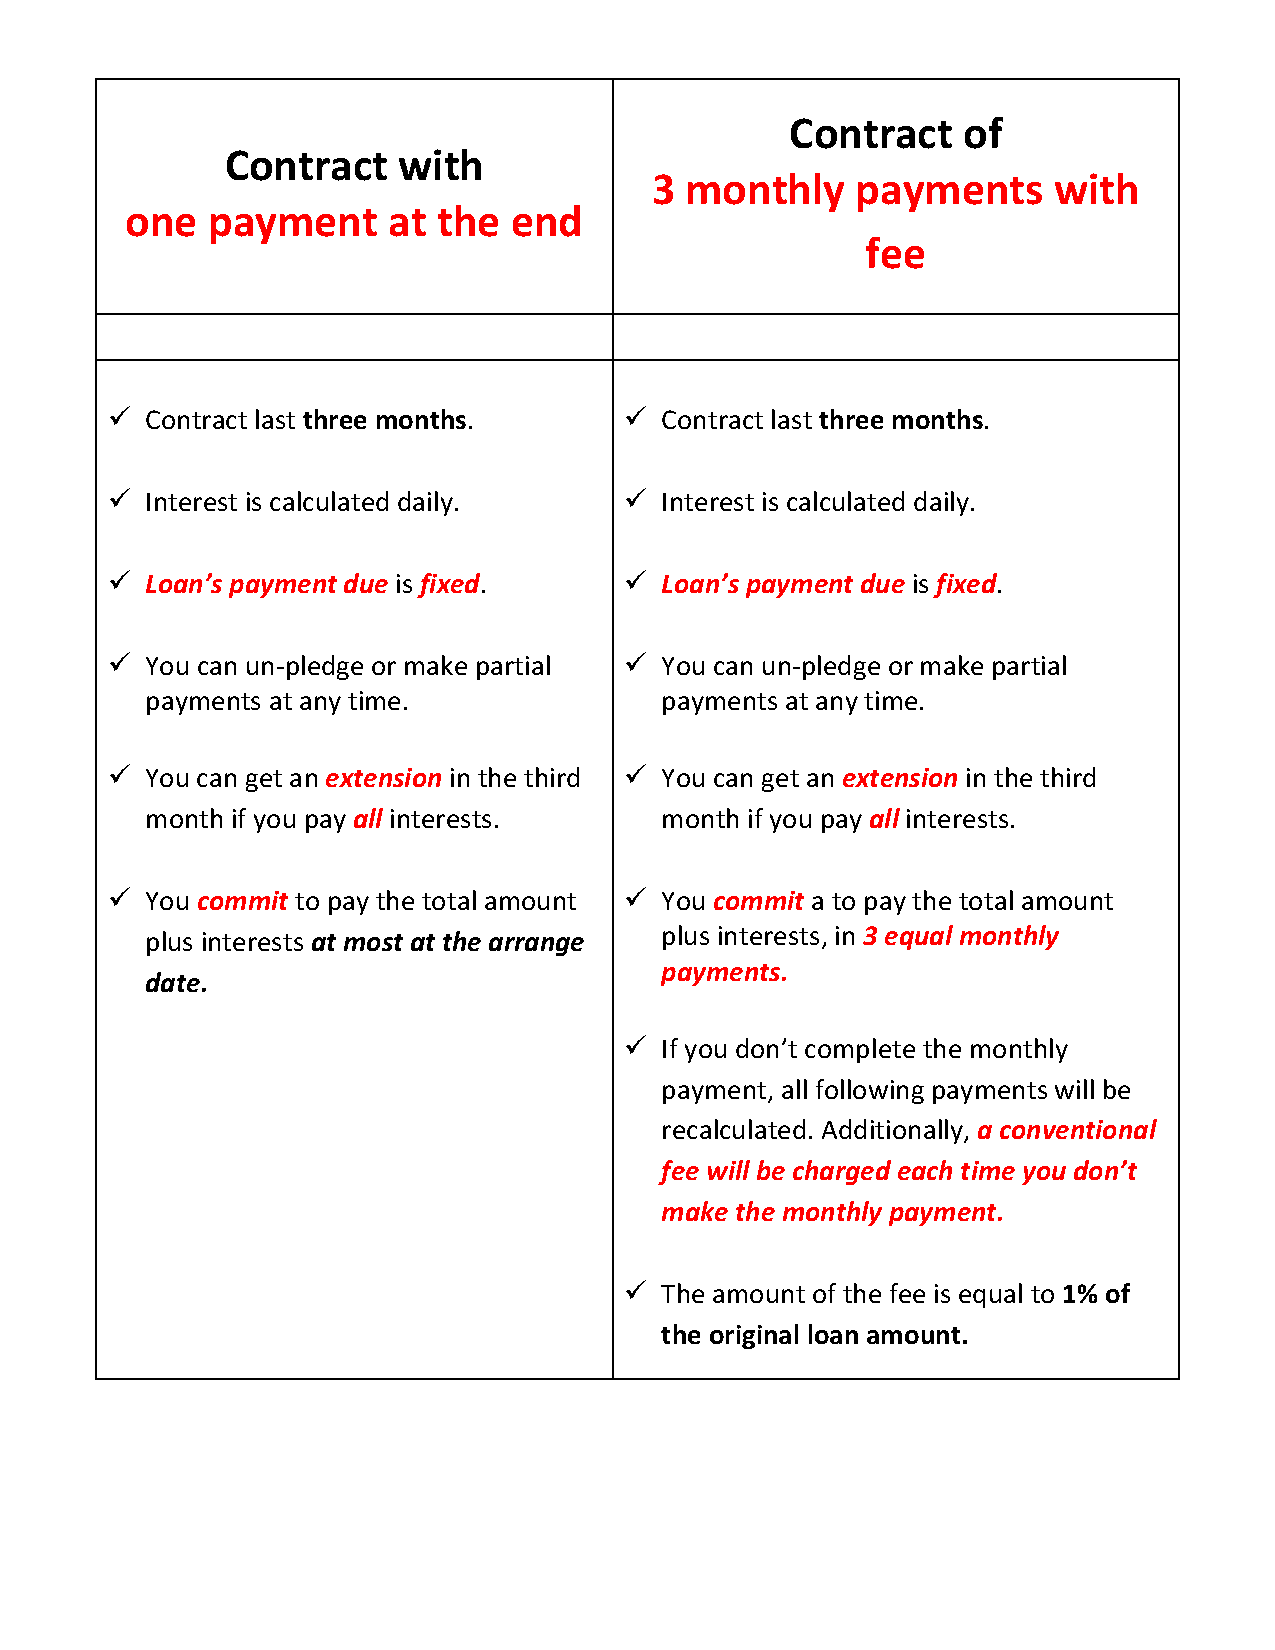
\includegraphics[width=\textwidth]{Figuras/MP_2.pdf}
    %\end{subfigure}
%    \end{center}
%\end{figure}



\subsection{Surveys}


%\begin{table}[H]
%\caption{Survey's non-response balance}
%\label{balance_response}
%\begin{center}
%\scriptsize{% Table generated by Excel2LaTeX from sheet 'balance_response'
\begin{tabular}{lcccc|ccc}
\toprule
      &       & \multicolumn{3}{c|}{Panel A : Entry Survey} & \multicolumn{3}{c}{Panel B : Exit Survey} \\
\midrule
\midrule
      & Overall & No Response & Response & p-value & No Response & Response & p-value \\
\midrule
\midrule
Loan amount  & 2145.46 & 2262.14 & 2145.46 & 0.08  & 2157.15 & 2367.62 & 0.17 \\
      & (31.81) & (59.21) & (35.45) &       & (30.93) & (154.83) &  \\
Monday & 0.18  & 0.18  & 0.18  & 0.95  & 0.18  & 0.19  & 0.71 \\
      & (0.02) & (0.03) & (0.02) &       & (0.02) & (0.04) &  \\
Number of branch-day pawns & 33.03 & 32.13 & 33.33 & 0.61  & 32.83 & 35.66 & 0.51 \\
      & (1.04) & (2.08) & (1.2) &       & (1.07) & (4.18) &  \\
\midrule
Obs   & 13444 & 3007  & 10437 &       & 12539 & 905   &  \\
\bottomrule
\bottomrule
\end{tabular}%
}
%\end{center}
% \scriptsize This table shows whether the means of variables in the administrative dataset are different for those that respond the baseline survey vs those that do not. We use this as an assessment of external validity. Internal validity is guaranteed because the baseline survey was implemented before treatment assignment and therefore response rates are orthogonal to treatment assignments. Panel A studies the baseline survey, while Panel B focuses on the exit survey. The columns labeled ``p-values'' report p-values for the test that the means of the respective variable are the same for those that responded did not respond the survey.
%\textit{Do file: } \texttt{balance\_response.do}
%\end{table}


\afterpage{
\begin{table}[H]
\caption{Baseline survey}
\label{baseline_survey}
\begin{center}
\scriptsize{% Table generated by Excel2LaTeX from sheet 'transcribed'
\begin{tabular}{cl}
\toprule
      & \textbf{Baseline Survey} \\
\midrule
\midrule
1     & \textbf{Your pawn was:} \\
      & (a) Inherite, (b) a gift, (c) bought by me, (d) lend to me, (e) other \_\_\_\_\_\_\_\_\_\_\_\_ \\
2     & \textbf{Mark with an "X" in the line below how likely is that you recover your pawn. } \\
      & \textbf{Where 0 is impossible and 100 is completely certain} \\
3     & \textbf{How much do you think the item you plan to pawn is worth?       \_\_\_\_\_\_\_\_\_\_\_\_\_\_ pesos} \\
4     & \textbf{Gender      } \\
5     & \textbf{Age} \\
6     & \textbf{Civil Status } \\
      & (a) married, (b) single, (c) divorced, (d) widowed \\
7     & \textbf{Work status} \\
      & (a) employed, (b) own business, (c) houseshores, (d) don't work, (e) retired, (f) study \\
8     & \textbf{Education} \\
      & (a) no formal education, (b) primary, (c) middle school, (d) highschool, (e) more than highschool \\
9     & \textbf{In the last month, did a friend or family member asked you for money?} \\
      & (a) yes  (b) no \\
10    & \textbf{What would you like to have: 100 pesos tomorrow or 150 pesos in one month?} \\
11    & \textbf{How often do you feel stressed by your economic situation?} \\
      & (a) always, (b) very often, (c) sometimes, (d) never \\
12    & \textbf{What is the main reason you want to pawn?} \\
      & (a) Need the money because somebody in my family lost his/her job \\
      & (b) Need the money to pay for a sickness in the family \\
      & (c) Need the money for an urgent expense \\
      & (d) Need the money for some non urgent expense. \\
13    & \textbf{How stressed do you feel from the situation that led to to pawn?} \\
      & (a) very stressed, (b) somwhat stressed, (c) a little stressed, (d) not stressed  \\
14    & \textbf{In 3 months, I expect to have a  \_\_\_\_\_\_\_\_\_\_\_\_\_\_\_\_ situation} \\
      & (a) better, (b) similar,  (c) worse \\
15    & \textbf{Have you panwned before?} \\
      & (a) yes  (b) no \\
16    & \textbf{How many times have you pawned on a Lender P branch?} \\
      & (a) NO\_\_\_    (b)  1-2 times \_\_\_    (c) 3-5 times\_\_\_\_   (d) More than 5\_\_\_\_ \\
17    & \multicolumn{1}{p{54.91em}}{\textbf{If you are saving money and a family member wants to use it for something }} \\
      & \multicolumn{1}{p{54.91em}}{(a) I would only give him the money for an urgent expenze} \\
      & \multicolumn{1}{p{54.91em}}{(b) I would give him the money even if it was not an urgent expense} \\
      & \multicolumn{1}{p{54.91em}}{(c) I would not give him/her the money regardless} \\
      & \multicolumn{1}{p{54.91em}}{(d) No one would ask me for my money} \\
18    & \textbf{Do you make an expenses budget for the month ahead of time?} \\
      & (a) always, (b) very often, (c) sometimes, (d) never \\
19    & \multicolumn{1}{p{54.91em}}{\textbf{Do you have other items you could pawn?}} \\
      & (a) yes  (b) no \\
20    & \textbf{Do you have savings?} \\
      & (a) yes  (b) no \\
21    & \textbf{Do you participate in a ROSCA?} \\
      & (a) yes  (b) no \\
22    & \textbf{Is it common that family or friends ask for money?} \\
      & (a) yes  (b) no \\
23    & \textbf{How much did you spend to come to the branch today?    \$\_\_\_\_\_\_\_\_\_\_\_\_\_\_ pesos} \\
24    & \textbf{How much time does it usually take to come to this branch?    \_\_\_\_\_\_\_\_\_\_\_} \\
25    & \textbf{How much does your family spend in a normal week?   \$\_\_\_\_\_\_\_\_\_\_\_\_\_\_ pesos} \\
26    & \textbf{How much do you manage to save in a normal week?   \$\_\_\_\_\_\_\_\_\_\_\_\_\_\_ pesos} \\
27    & \textbf{Does it happen to you that you spend more than you wanted because you fall into temptation?} \\
      & (a) never, (b) almost never, (c) sometimes, (d) very often \\
28    & \textbf{In the last 6 months, has it happened that at some point you lacked money to pay} \\
      & (a) rent?    (b) food    (c)food   (d) medicine  (e) electricity   (f) heating   (g) telephone    (i) water \\
29    & \textbf{What would you like to have: 100 pesos in 3 months or 150 pesos in four months?} \\
30    & \textbf{Would you like to receive (free) reminders for upcomming payments?} \\
      & (a) yes  (b) no \\
\bottomrule
\end{tabular}%
}
\end{center}
\end{table}
}


\begin{comment}
\begin{table}[H]
\caption{Reincidence SS}
\label{tab_reincidence}
\begin{center}
\scriptsize{% Table generated by Excel2LaTeX from sheet 'tab_reincidence'
\begin{tabular}{lccccc}
\toprule
Variable & Obs   & Mean  & Std. Dev. & Min   & Max \\
\midrule
\midrule
Number of visits & 26179 & 1.72  & 1.27  & 1     & 7 \\
Received more one treatment arm & 26179 & 0.23  & 0.42  & 0     & 1 \\
Number of arms & 26179 & 1     & 1.06  & 0     & 5 \\
Reincidence & 16470 & 0.29  & 0.45  & 0     & 1 \\
Same product of reincidence & 16470 & 0.02  & 0.13  & 0     & 1 \\
Number of visits $<$ 75 days & 26179 & 2.1   & 1.5   & 1     & 7 \\
Received more one treatment arm $<$ 75 days & 26179 & 0.22  & 0.41  & 0     & 1 \\
Number of arms  $<$ 75 days & 26179 & 0.97  & 1.01  & 0     & 5 \\
Chose same treatment arm & 1066  & 0.45  & 0.5   & 0     & 1 \\
\bottomrule
\bottomrule
\end{tabular}%
}
\end{center}
 \scriptsize
%\textit{Do file: } \texttt{tab\_reincidence.do}
\end{table}


\begin{table}[H]
\caption{Summary statistics (exit survey)}
\label{SS_exit}
\begin{center}
\scriptsize{% Table generated by Excel2LaTeX from sheet 'SS'
\begin{tabular}{lccccccc}
\toprule
\multicolumn{8}{c}{Exit Survey Data} \\
\midrule
\midrule
      &       &       & \multicolumn{2}{c}{No Choice } & \multicolumn{2}{c}{Choice} &  \\
\midrule
\midrule
      & Overall & Control & Fee   & Promise & Fee   & Promise & p-value \\
\midrule
      & \multicolumn{7}{c}{Panel A: Outcomes} \\
\midrule
\midrule
Will reincide & 0.94  & 0.96  & 0.95  & 0.96  & 0.94  & 0.92  & 0.6 \\
      & (0.01) & (0.01) & (0.02) & (0.02) & (0.02) & (0.03) &  \\
Very satisfied & 0.34  & 0.36  & 0.32  & 0.33  & 0.33  & 0.36  & 0.95 \\
      & (0.02) & (0.05) & (0.05) & (0.05) & (0.04) & (0.04) &  \\
Better econ situation & 0.42  & 0.53  & 0.29*** & 0.35** & 0.44  & 0.47  & 0.02 \\
      & (0.03) & (0.06) & (0.05) & (0.06) & (0.05) & (0.04) &  \\
Choose frequent payment & 0.63  & 0.65  & 0.58  & 0.58  & 0.58  & 0.77** & 0 \\
      & (0.02) & (0.05) & (0.05) & (0.06) & (0.04) & (0.03) &  \\
\midrule
      & \multicolumn{7}{c}{Panel B: Balance} \\
\midrule
\midrule
Loan amount  & 1957.72 & 1940.41 & 1926  & 2006.83 & 2002.97 & 1892.54 & 0.98 \\
      & (67.84) & (160.03) & (150.89) & (187.56) & (114.96) & (157.83) &  \\
Woman & 0.71  & 0.69  & 0.72  & 0.77  & 0.66  & 0.73  & 0.58 \\
      & (0.02) & (0.05) & (0.06) & (0.05) & (0.05) & (0.04) &  \\
Age   & 43.98 & 42.84 & 46.27 & 43.82 & 44.57 & 42.24 & 0.29 \\
      & (0.59) & (1.33) & (1.74) & (1.1) & (0.99) & (1.16) &  \\
Subjective value & 3166.31 & 3448.99 & 3182.11 & 3049.88 & 3074.69 & 3081.52 & 0.85 \\
      & (120.82) & (288.38) & (286.2) & (303.87) & (210.79) & (296.63) &  \\
Has pawn before & 0.88  & 0.84  & 0.9   & 0.87  & 0.95** & 0.8   & 0.01 \\
      & (0.02) & (0.05) & (0.03) & (0.05) & (0.02) & (0.05) &  \\
Subj. pr. of recovery & 95.35 & 94.5  & 94.84 & 96.6  & 95.06 & 95.87 & 0.82 \\
      & (0.56) & (1.4) & (1.21) & (1.5) & (1.01) & (1.09) &  \\
+High-school & 0.66  & 0.72  & 0.63  & 0.65  & 0.67  & 0.64  & 0.84 \\
      & (0.03) & (0.06) & (0.06) & (0.07) & (0.05) & (0.06) &  \\
\midrule
Obs   & 905   & 175   & 154   & 172   & 234   & 170   &  \\
\bottomrule
\bottomrule
\end{tabular}%
}
\end{center}
 \scriptsize We carried out an exit survey. It had a small response rate and we don't use it in the paper. Here it shows that the characteristics of those that responded it are balanced across arms (Panel B). Panel A reports outcomes.
%\textit{Do file: } \texttt{ss.do}
\end{table}
\end{comment}


\newpage
\subsection{Some more evidence of overconfidence}

\vspace{.2in}
\begin{figure}[H]
    \caption{Behavior of those who lost pawn}
    \label{proxy_naive}
    \begin{center}
    \begin{subfigure}{0.40\textwidth}
        \caption{Elapsed days to first payment}
        \centering
        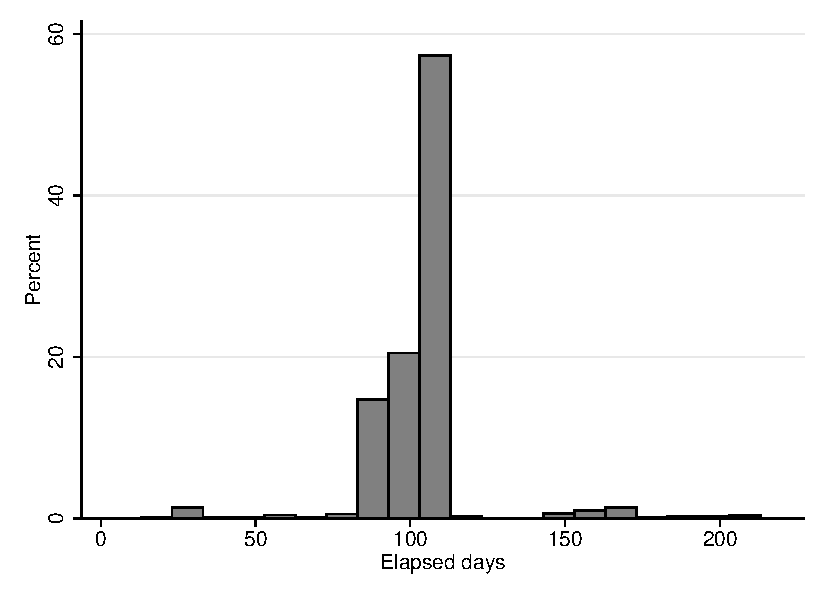
\includegraphics[width=\textwidth]{Figuras/hist_firstdays_default.pdf}
    \end{subfigure}
    \begin{subfigure}{0.40\textwidth}
        \caption{Elapsed days to last payment}
        \centering
        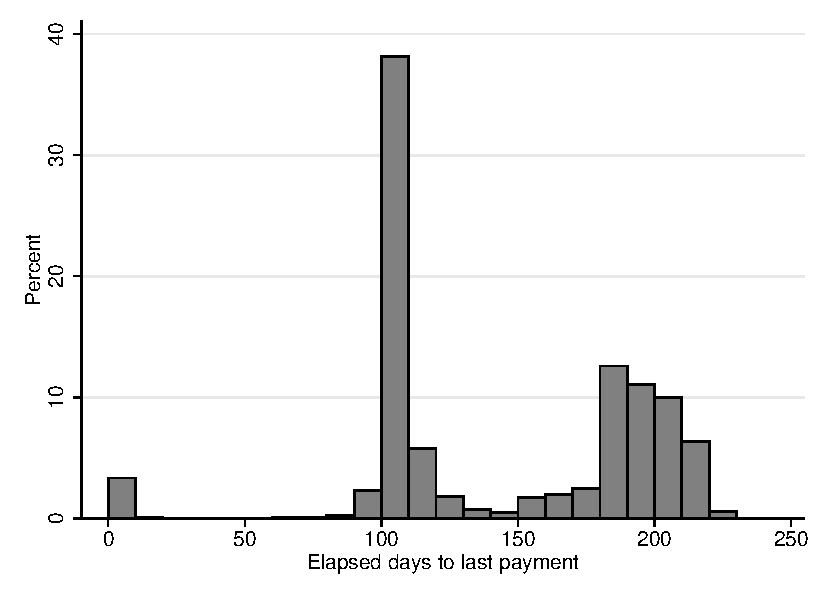
\includegraphics[width=\textwidth]{Figuras/hist_days_default.pdf}
    \end{subfigure}
        \begin{subfigure}{0.40\textwidth}
        \caption{Payments as \% of loan}
        \centering
        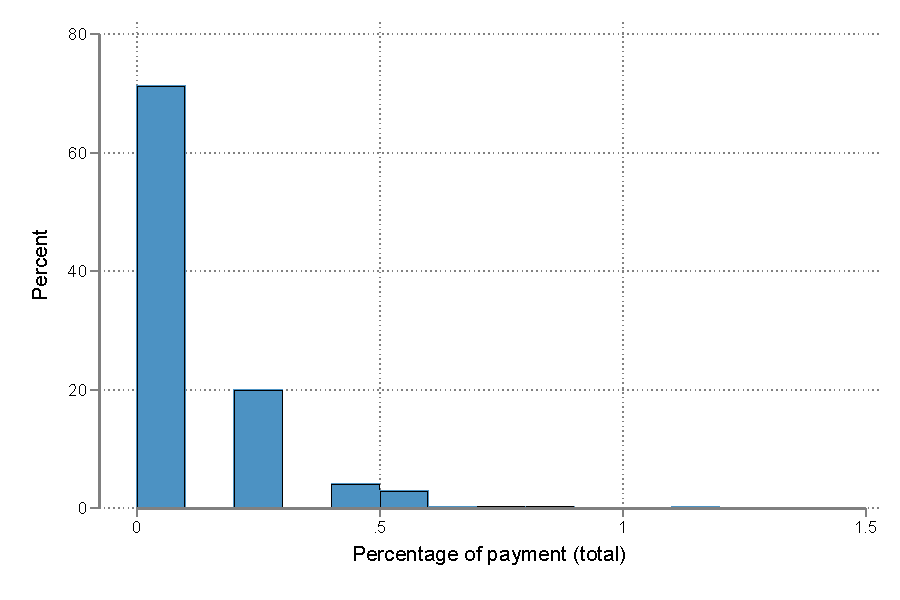
\includegraphics[width=\textwidth]{Figuras/hist_percpay_default.pdf}
    \end{subfigure}
    \begin{subfigure}{0.40\textwidth}
        \caption{Number of payments}
        \centering
        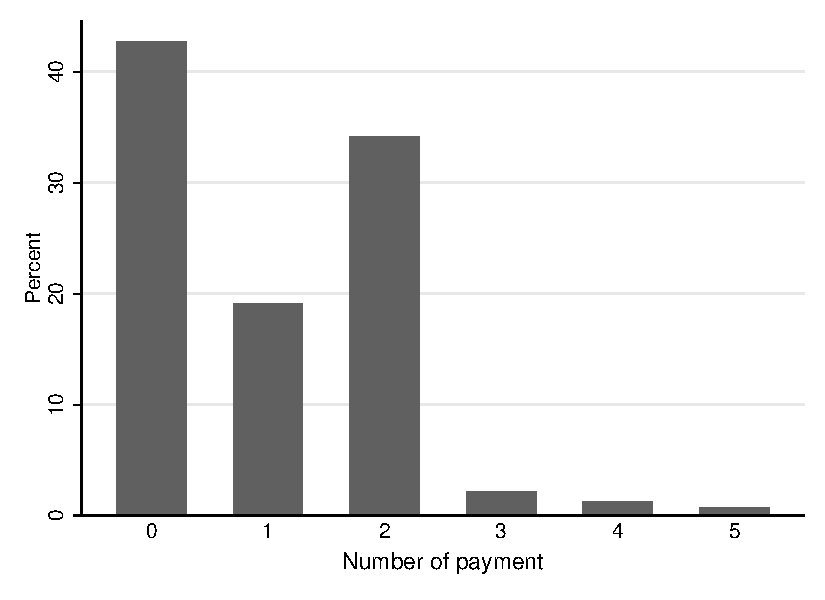
\includegraphics[width=\textwidth]{Figuras/hist_numpay_default.pdf}
    \end{subfigure}
    \end{center}
        \scriptsize 
        This figure describes behavior for the subsample of clients whose pawn was not recovered (in the control group).  Panel (a) shows days elapsed from the pawn to the first payment, while panel (b) displays the days elapsed to last payment. Some people pay after the day 105 when the grace period ends because the can ``restart'' the loan if they pay all interest owed. It amounts to starting a new loan with the same conditions and same pawn. Panel (c) shows the fraction of the loan that they paid (even when they ended up losing the pawn). Panel (d) displays the number of times they went to the branch to pay.      
      %\textit{Do file: }  \texttt{hist\_den\_default.do}
\end{figure}


\newpage
\subsection{Main treatment effects: Additional material}



% \begin{figure}[H]
%         \caption{FC restricted to 115 days}
%     \label{fc_pro_2_115}
%     \begin{center}
%         \centering
%         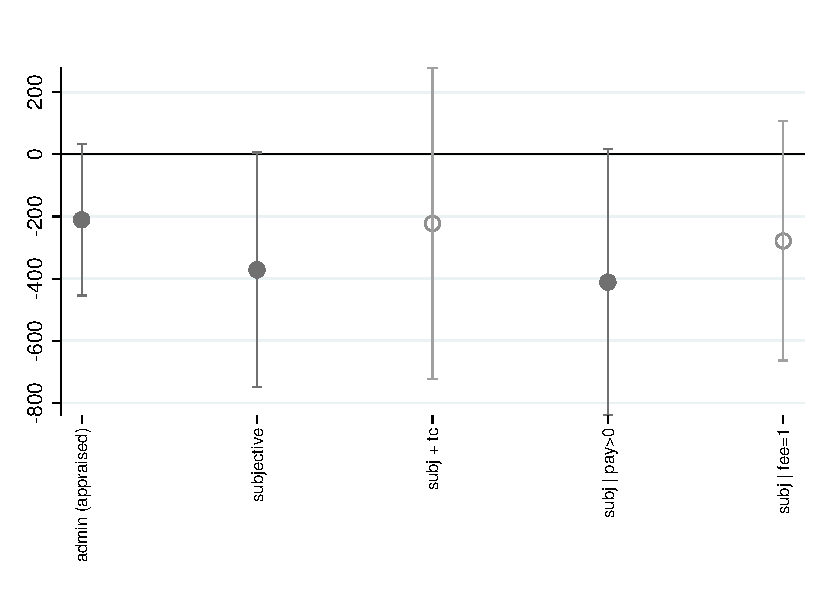
\includegraphics[width=0.50\textwidth]{Figuras/fc_te_115_pro_2.pdf}
%     \end{center}
%      \scriptsize This figure is the same as in Figure \ref{fc_pro2} Panel (a), but with the subsample restricted to the first 115 days.
%      %\textit{Do file: }  \texttt{fc\_te\_115.do}
% \end{figure}



% \begin{figure}[H]
%         \caption{Financial cost effect: charging all fees}
%     \label{fc_allfee}
%     \begin{center}
%         \centering
%         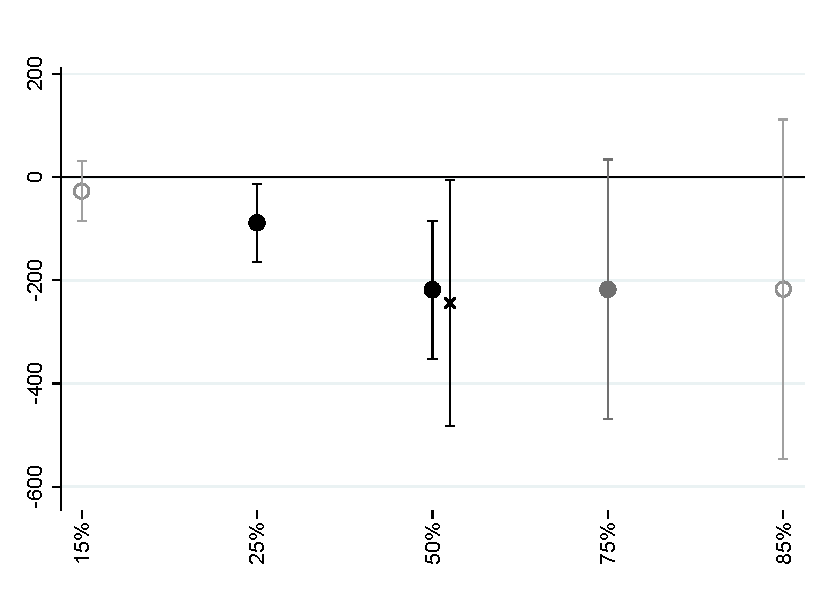
\includegraphics[width=0.50\textwidth]{Figuras/fc_allfee_quantile_pro_2.pdf}
%     \end{center}
%     \scriptsize
%      This figure is the analogous to Figure \ref{fc_pro2}(b), except that for the fee-forcing contract we pretend that all clients incurred in their late fees, and therefore inflate the financial cost by summing those fees. This is intended as a kind of worse case scenario for the financial cost of the fee-forcing contract. The circles indicate the quantile treatment effects, while the cross is the (OLS) mean. We still find that the financial cost of will be smaller under the fee-forcing contract in spite of artificially inflating it.
%      %\texttt{fc\_all\_fee.do}
% \end{figure}





% \begin{figure}[H]
%         \caption{FC as \% of loan - treatment effect}
%     \label{fc_perc}
%     \begin{center}
%         \centering
%         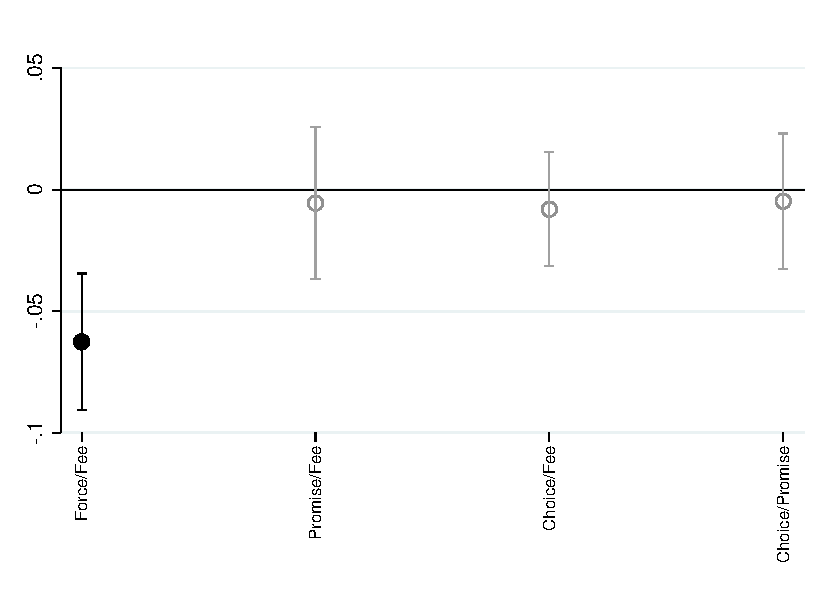
\includegraphics[width=0.50\textwidth]{Figuras/fc_perc_te_allarms.pdf}
%     \end{center}
%      \scriptsize This figure shows the estimated treatment effect of all arms against the status quo, but normalizing the dependent variable by the value of the loan.
%      %\textit{Do file: }  \texttt{fc\_perc\_allarms.do}
% \end{figure}




\begin{figure}[H]
    \caption{Relationship between treatment effects}
    \label{induced_to_pay_early}
    \begin{center}
    \begin{subfigure}{0.45\textwidth}
        \caption{\footnotesize{Induced to pay earlier vs Induced Lower FC}}
        \centering
        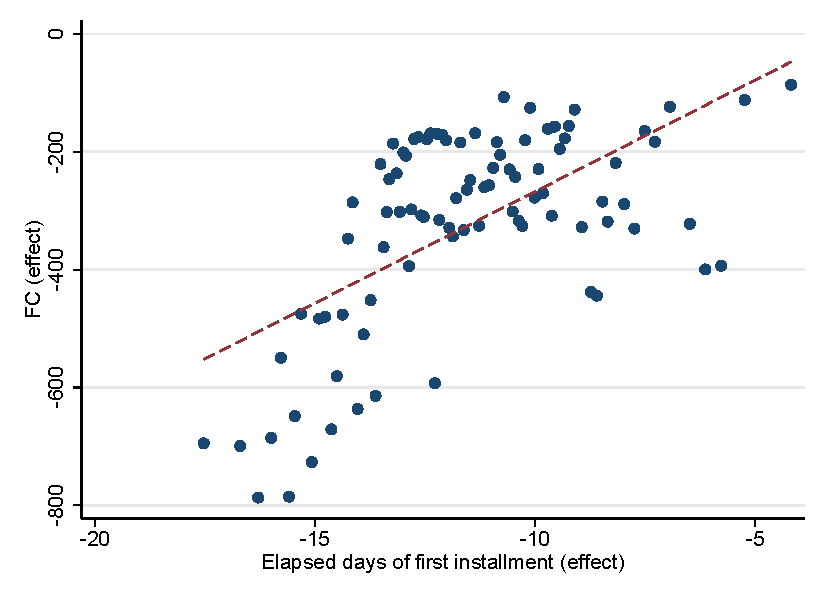
\includegraphics[width=\textwidth]{Figuras/binscatter_fc_days_pro_2.pdf}
    \end{subfigure}
        \begin{subfigure}{0.45\textwidth}
        \caption{\footnotesize{Induced to pay earlier vs Induced Recovery}}
        \centering
        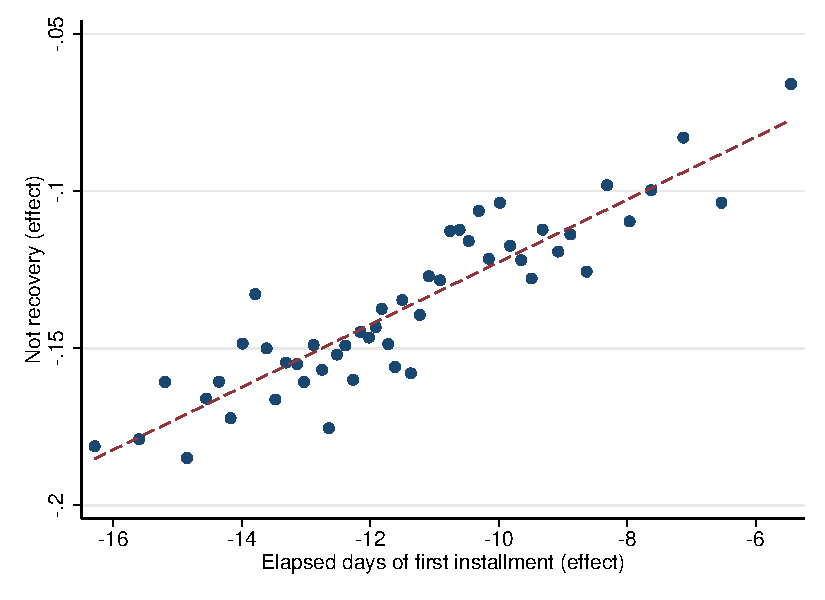
\includegraphics[width=\textwidth]{Figuras/binscatter_def_days_pro_2.pdf}
    \end{subfigure}
    \end{center}
       \scriptsize 
       This figure plots relationships between \textit{treatment effects}. Both Panels (a) an (b) have the same X-axis, which displays the estimated heterogeneous treatment effect on the outcome ``elapsed days of first payment'', that is how many days elapsed from the day the loan was awarded to the first payment the client made. The treatments effects were calculated using \cite{atheygrf}. In Panel (a) the Y-axis is the \textit{treatment effect} on financial cost. In Panel (b) the Y-axis is the \textit{treatment effect} on losing their pawn. Panel (a) shows that those induced to pay earlier are also those that have larger savings in financial cost as a result of ``forcing'' the frequent payment commitment contract compared to the status-quo (control). Panel (b) shows that those induced to pay earlier are also those that have a larger increase in recovery.
      %\textit{Do file: }  \texttt{binscatter\_hte.do}
\end{figure}

\begin{figure}[H]
        \caption{Repeat purchase before 30/60 days}
    \label{reincidence_before}
    \begin{center}
        \centering
        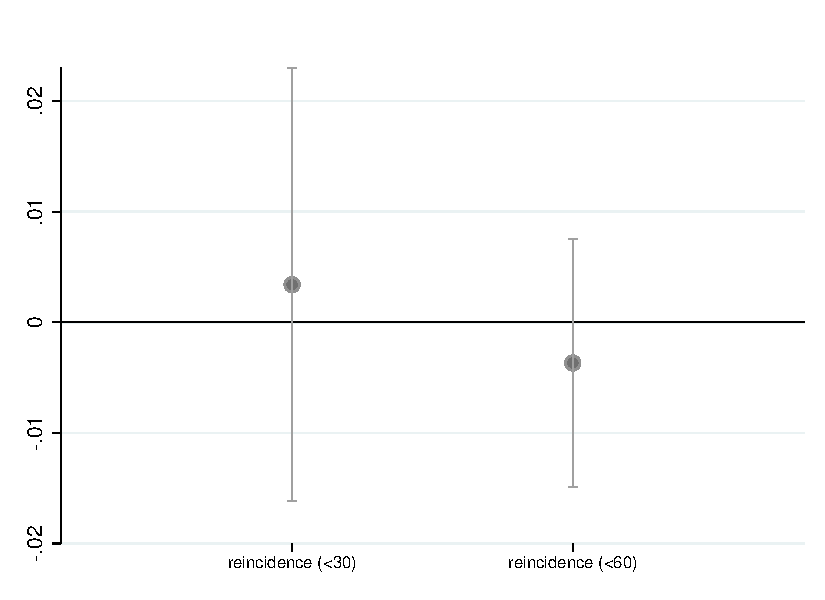
\includegraphics[width=0.50\textwidth]{Figuras/re_te_earlydays.pdf}
    \end{center}
     \scriptsize This figure shows the estimated treatment effect of repeat purchase before 30 \& 60 days.
     %\textit{Do file: }  \texttt{re\_te\_earlydays.do}
\end{figure}




\vspace{.3in}

\subsection{FOSD: fee forcing vs status quo financial cost distributions}


\vspace{.2in}
\begin{figure}[H]
        \caption{Empirical CDF of Financial Cost: fee-focing vs status-quo}
    \label{ecdf_fc}
    \begin{center}
        \centering
        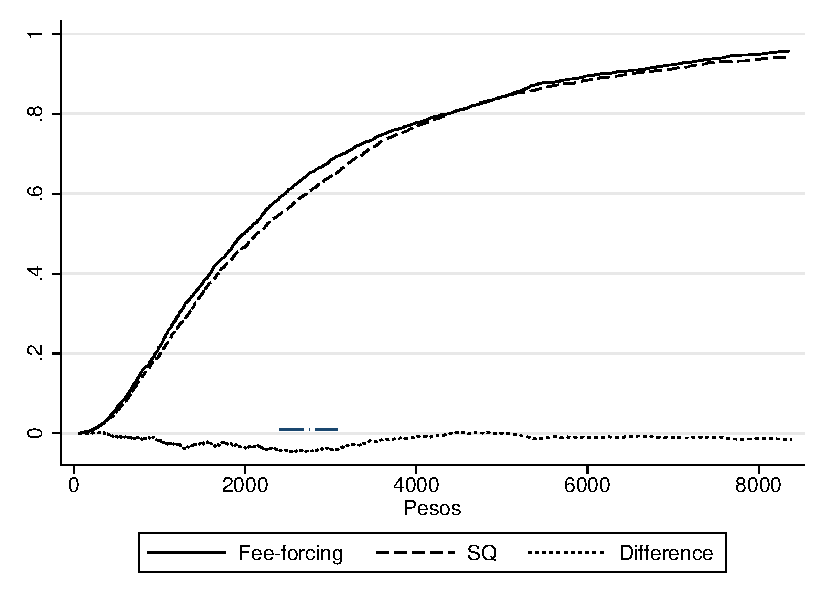
\includegraphics[width=0.65\textwidth]{Figuras/cdf_fc_pro_2.pdf}
    \end{center}
    \scriptsize This figure plots the empirical cumulative distribution of financial cost. It does this separately for the fee-forcing contract and for the status-quo contract. The doted line at the bottom is the difference of the status-quo CDF minus the fee-forcing CDF. It shows that the CDF of the status quo contract is always below that of the fee-forcing (and this difference is significant for the points indicated by the blue line), and therefore that the former first-order stochastically dominates the later for weakly decreasing utility functions; see Proposition \ref{eq_fosd}.
    % \texttt{ecdf\_fc.do}}
\end{figure}

\begin{figure}[H]
        \caption{Empirical CDF of APR: fee-focing vs status-quo}
    \label{ecdf_fc}
    \begin{center}
        \centering
        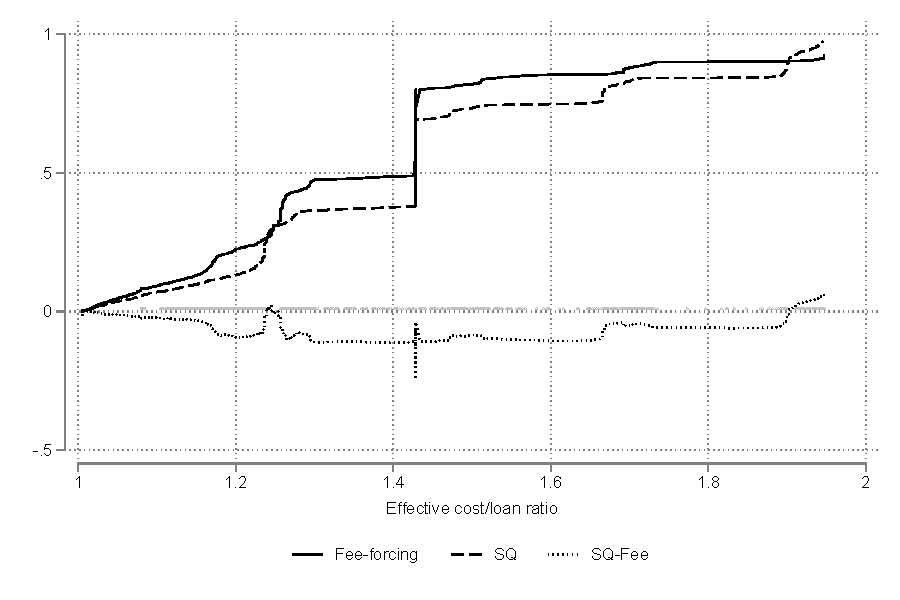
\includegraphics[width=0.65\textwidth]{Figuras/cdf_eff_pro_2.pdf}
    \end{center}
    \scriptsize This figure plots the empirical cumulative distribution of financial cost. It does this separately for the fee-forcing contract and for the status-quo contract. The doted line at the bottom is the difference of the status-quo CDF minus the fee-forcing CDF. It shows that the CDF of the status quo contract is always below that of the fee-forcing (and this difference is significant for the points indicated by the blue line), and therefore that the former first-order stochastically dominates the later for weakly decreasing utility functions; see Proposition \ref{eq_fosd}.
    % \texttt{ecdf\_fc.do}}
\end{figure}


\vspace{.2in}
\begin{table}[H]
\caption{Clients who should prefer fee-forcing financial cost distribution}
\label{stochastic_dominance}
\begin{center}
\scriptsize{% Table generated by Excel2LaTeX from sheet 'dominance'
\begin{tabular}{lccc}
\toprule
Sub-population & Dominance & Log-normality (AD/KS) & Obs \\
\midrule
\midrule
Fee-forcing & \cellcolor[rgb]{ .557,  .663,  .859} $\succeq_{1}^*$ & */*  |  */* & 5034 \\
Low-loan & $\succeq_{1}^*$ &    /     |     /    & 2508 \\
High-loan & $\succeq_{1}^*$ &    /     |     /    & 2526 \\
Low-subj. prob. & \cellcolor[rgb]{ .557,  .663,  .859} $\succeq_{1}^*$ & */*  |  */* & 1083 \\
High-subj. Prob. & \cellcolor[rgb]{ .557,  .663,  .859} $\succeq_{1}^*$ & */*  |  */* & 2590 \\
Low-age & $\preceq_{1}$ & */*  |  */* & 1358 \\
High-age & \cellcolor[rgb]{ .851,  .882,  .949} $\succeq_{1}$ & */*  |     /* & 1362 \\
Low-income index & \cellcolor[rgb]{ .851,  .882,  .949} $\succeq_{1}$ & */*  |  */* & 1047 \\
High-income index & \cellcolor[rgb]{ .851,  .882,  .949} $\succeq_{1}$ & */*  |  */* & 948 \\
Male  & -     & */*  |     /* & 755 \\
Female & \cellcolor[rgb]{ .851,  .882,  .949} $\succeq_{1}$ & */*  |  */* & 2158 \\
First time & $\preceq_{1}$ & */*  |  */* & 293 \\
Pawn before & \cellcolor[rgb]{ .851,  .882,  .949} $\succeq_{1}$ & */*  |  */* & 2475 \\
Family doesn't ask & $\preceq_{1}$ & */*  |  */* & 1826 \\
Family asks & \cellcolor[rgb]{ .557,  .663,  .859} $\succeq_{1}^*$ & */*  |  */* & 987 \\
Not common ask & \cellcolor[rgb]{ .851,  .882,  .949} $\succeq_{1}$ & */*  |  */* & 1436 \\
Common asks & -     & */*  |  */* & 625 \\
No savings & $\preceq_{1}$ & */*  |  */* & 1353 \\
Has savings & \cellcolor[rgb]{ .557,  .663,  .859} $\succeq_{1}^*$ & */*  |  */* & 717 \\
Not rosca & \cellcolor[rgb]{ .557,  .663,  .859} $\succeq_{1}^*$ & */*  |  */* & 1270 \\
Rosca & $\preceq_{1}$ & */*  |  */* & 795 \\
Low-education & \cellcolor[rgb]{ .851,  .882,  .949} $\succeq_{1}$ & */*  |     /* & 906 \\
High-education & \cellcolor[rgb]{ .851,  .882,  .949} $\succeq_{1}$ & */*  |  */* & 1797 \\
Not stressed & -     & */*  |  */* & 1998 \\
Stressed & -     & */*  |  */* & 839 \\
Not overconfident & $\preceq_{1}$ & */*  |  */* & 47 \\
Overconfident & \cellcolor[rgb]{ .851,  .882,  .949} $\succeq_{1}$ & */*  |     /* & 1626 \\
Not PB & \cellcolor[rgb]{ .851,  .882,  .949} $\succeq_{1}$ & */*  |  */* & 1438 \\
PB    & \cellcolor[rgb]{ .557,  .663,  .859} $\succeq_{1}^*$ & */*  |     /* & 226 \\
Not FB & \cellcolor[rgb]{ .851,  .882,  .949} $\succeq_{1}$ & */*  |  */* & 1521 \\
FB    & \cellcolor[rgb]{ .851,  .882,  .949} $\succeq_{1}$ & */*  |  */* & 143 \\
Doesn't make budget & \cellcolor[rgb]{ .851,  .882,  .949} $\succeq_{1}$ & */*  |  */* & 1054 \\
Makes budget & \cellcolor[rgb]{ .851,  .882,  .949} $\succeq_{1}$ & */*  |  */* & 1689 \\
Not tempted & \cellcolor[rgb]{ .851,  .882,  .949} $\succeq_{1}$ & */*  |     /* & 875 \\
Tempted & \cellcolor[rgb]{ .851,  .882,  .949} $\succeq_{1}$ & */*  |  */* & 1872 \\
High-transp. cost & \cellcolor[rgb]{ .851,  .882,  .949} $\succeq_{1}$ & */*  |  */* & 1352 \\
Low-transp. cost & \cellcolor[rgb]{ .851,  .882,  .949} $\succeq_{1}$ & */*  |  */* & 1343 \\
High-transp. time & \cellcolor[rgb]{ .851,  .882,  .949} $\succeq_{1}$ & */*  |  */* & 1260 \\
Low-transp. time & \cellcolor[rgb]{ .557,  .663,  .859} $\succeq_{1}^*$ & */*  |  */* & 1442 \\
\bottomrule
\bottomrule
\end{tabular}%
}
\end{center}
 \footnotesize
This table does two things. First, it tests whether the observed empirical distribution of financial cost is well approximated by a log normal. It does this using two tests, the Anderson-Darling and the Kolmogorov-Smirnoff tests. Second, it fits a log normal distribution by maximum likelihood to observed empirical distribution of financial cost, separately for the fee-forcing arm and the status-quo arm. Using the fitted log normal, it tests whether the fee-forcing financial cost distribution would be preferred by any expected utility agent using Proposition \ref{lognormal_fosd} below. The different rows of the table do this for different sub-populations.  The first row of the table does it for every client in the fee forcing and status quo arms. The ``*'' show that we cannot reject at the 5\% level that both distribution are log normal for any of the two tests. The column entitled ``Dominance'' shows whether any client that dislikes higher cost would prefer the fee-forcing cost distribution over the status quo one, with $\succeq_{1}$ meaning he should (with $\succeq_{1}^*$ indicating the difference is statistically significant). It turns out to be the case that for the overwhelming majority of sub-populations, the conditions of preferring the fee-forcing distribution hold.
%\textit{Do file: } \texttt{stoch\_dominance.do}
\end{table}


\vspace{.2in}
\begin{prop}
\label{lognormal_fosd}
\footnotesize{
Let $F$ and $G$ be the cumulative distributions of two alternative log-normal prospects. The following are equivalent:

\begin{enumerate}[(a)]
    \item For every weakly decreasing utility function $u$: $E_{F}(u(FC))\leq E_G(u(FC))$
    \item $E_F \log(FC)\geq E_G\log(FC)$ and $Var_F \log(FC)= Var_G\log(FC)$
\end{enumerate}
}
\end{prop}

\begin{proof}
\footnotesize{
See Theorem 4 in \cite{lognormal_dominance}.
}
\end{proof}

\newpage

\vspace{.1in}
\begin{prop}
\label{eq_fosd}
\footnotesize{
This is a standard result. 
\\
\vspace{.1in}
The following are equivalent:
\begin{enumerate}[(a)]
    \item For every weakly decreasing utility function $u$: $E_{sq}(u(FC))\leq E_{fee}(u(FC))$
    \item $F_{sq}(FC)\leq F_{fee}(FC)$ 
\end{enumerate}
}
\end{prop}
\begin{proof} \;
\footnotesize{

[$(a)\Longrightarrow (b)$] Suppose  $(b)$ does not hold. So there exists $FC^*$ such that $F_{sq}(FC^*)>F_{fee}(FC^*)$, Define $u:=\mathds{1}_{FC\leq FC^*}$. Then
\[E_{sq}(u(FC)) = \int u(FC)dF_{sq} = F_{sq}(FC^*)>F_{fee}(FC^*)= \int u(FC)dF_{fee} =E_{fee}(u(FC))\]
which contradicts $(a)$.\\

[$(a)\Longleftarrow (b)$] On the other hand for $u$ weakly decreasing,

\[\int u(y(FC))dF_{sq}(y(FC)) = \int u(y(FC))dF_{fee}(FC) \leq \int u(FC)dF_{fee}(FC)\]
with $y(FC) = F_{sq}^{-1}F_{fee}(FC)$.
}
\end{proof}
\footnotesize{
Note the proof was done in the case of absolutely continuous and strictly increasing distribution functions $F_{sq}$ and $F_{fee}$.
}




\newpage
\subsection{Causal Random Forest and HTE}

\vspace{.3in}
\begin{figure}[H]
        \caption{Honest causal tree for the Forced-commitment contract heterogeneous treatment effects}
    \label{casual_tree}
    \begin{center}
        \centering
        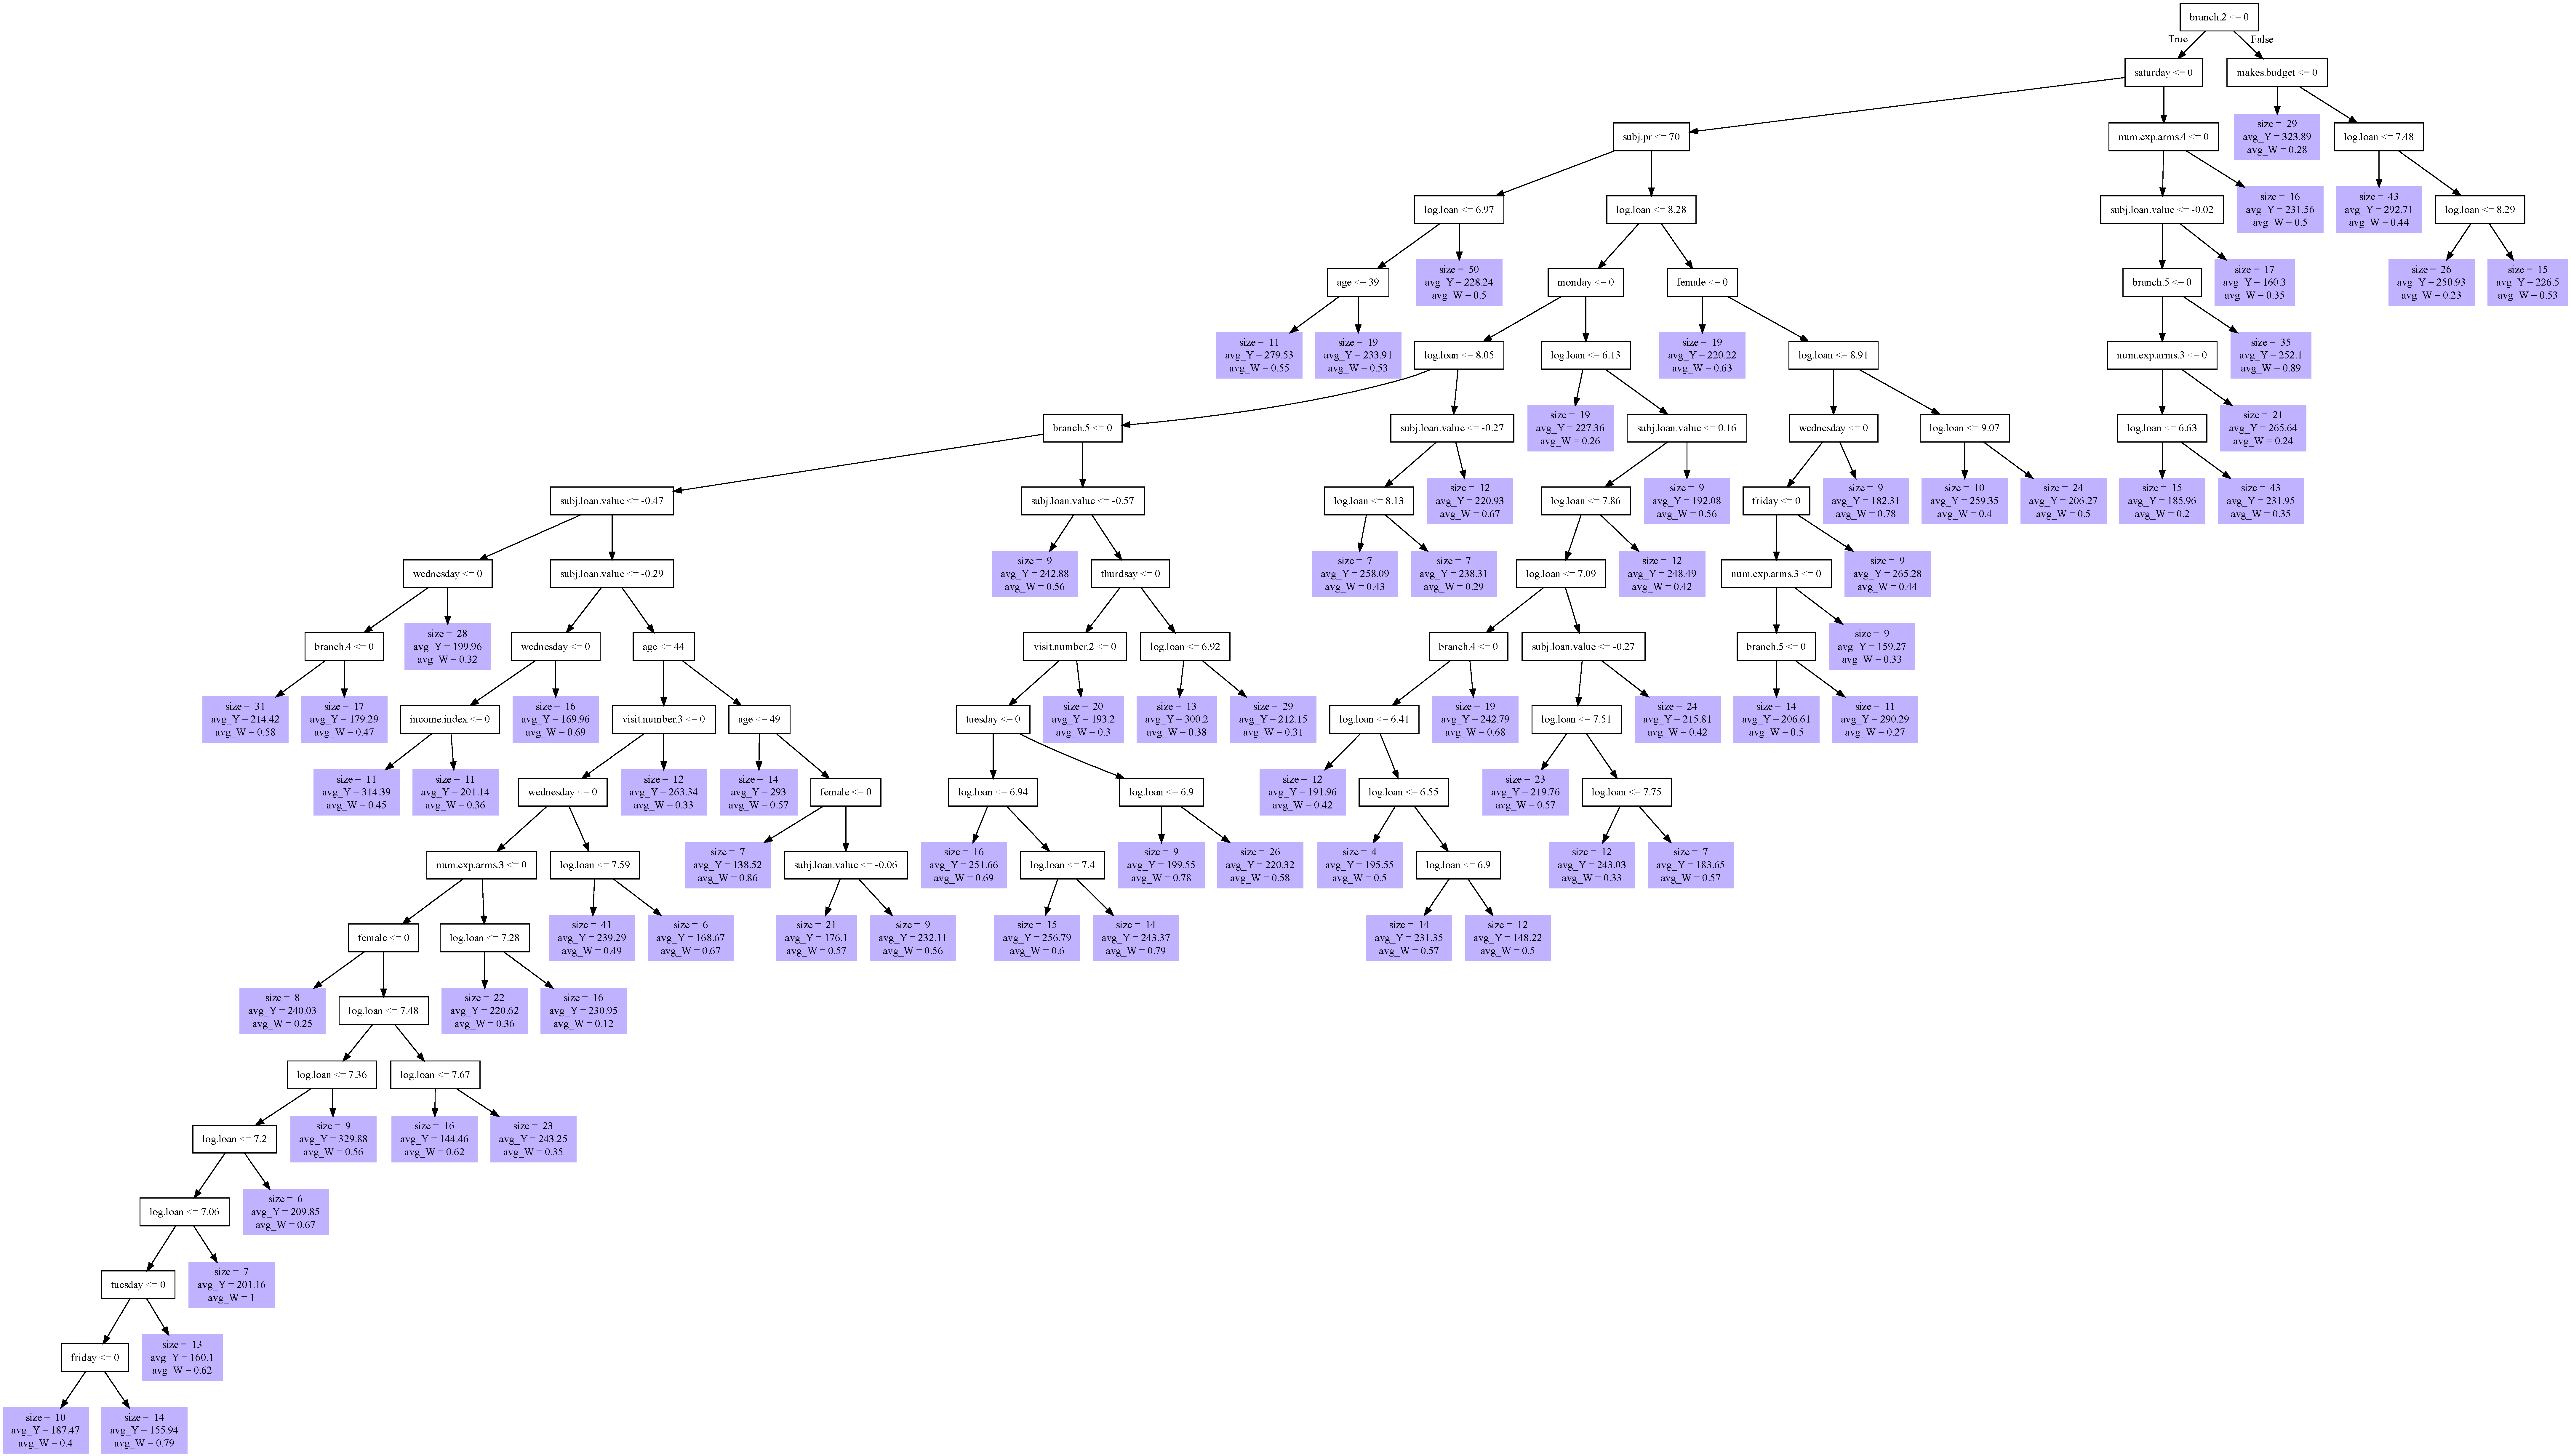
\includegraphics[width=\textwidth]{Figuras/crf_pro_2_apr.pdf}
    \end{center}
    \footnotesize 
    This is one(it is chosen such that it minimizes the pruned cost, that is it is the tree with the smallest root-node impurity) of the honest causal trees in the random forest we use for the estimation of the heterogeneous treatment effect of the fee-forcing contract. It is meant only as an example of how these trees look like. The forest was such that there are as many estimated treatment effects as there are clients.
     %\footnotesize{ \textit{RScript: }  \texttt{grf.R}
\end{figure}

We use \cite{atheygrf} \texttt{causal\_forest} of the \texttt{grf} library in $R$. The parameters used were:
\scriptsize{\textit{causal\_forest(
  X, 
  Y, 
  W, 
  Y.hat = NULL, 
  W.hat = NULL, 
  num.trees = 2000, 
  sample.weights = NULL, 
  clusters = NULL, 
  equalize.cluster.weights = FALSE, 
  sample.fraction = 0.5, 
  mtry = min(ceiling(sqrt(ncol(X)) + 20),ncol(X)), 
  min.node.size = 5, 
  honesty = TRUE, 
  honesty.fraction = 0.5, 
  honesty.prune.leaves = TRUE, 
  alpha = 0.05, 
  imbalance.penalty = 0, 
  stabilize.splits = TRUE, 
  ci.group.size = 2, 
  tune.parameters = "none", 
  tune.num.trees = 200, 
  tune.num.reps = 50, 
  tune.num.draws = 1000, 
  compute.oob.predictions = TRUE, 
  orthog.boosting = FALSE, 
  num.threads = NULL)}}


\begin{figure}[H]
        \caption{Single causal tree for the Forced-commitment contract heterogeneous treatment effects}
    \label{casual_tree}
    \begin{center}
        \centering
        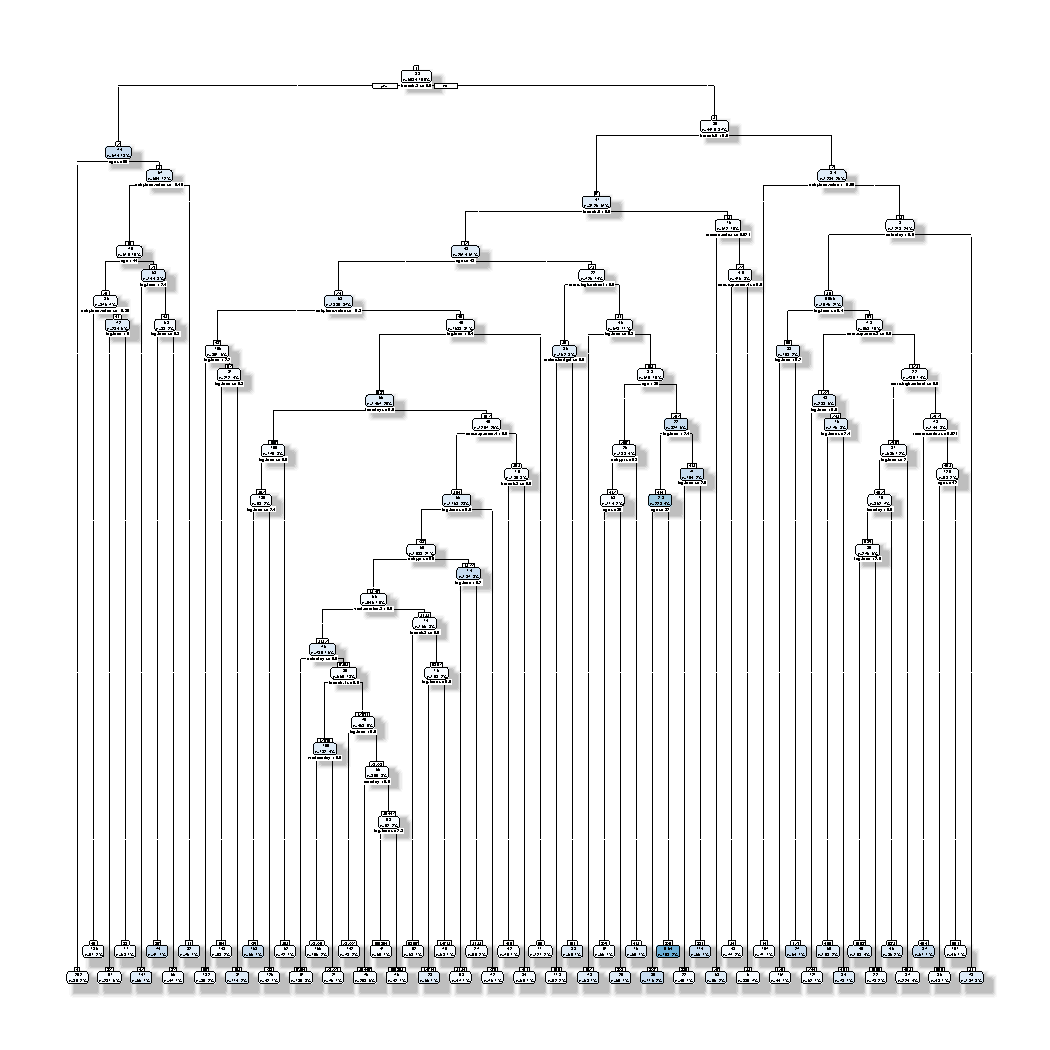
\includegraphics[width=\textwidth]{Figuras/ct_pro_2_apr.pdf}
    \end{center}
    \footnotesize 
   
     %\footnotesize{ \textit{RScript: }  \texttt{grf.R}
\end{figure}



% \begin{figure}[H]
%     \caption{Heterogeneous Treatment Effect: Fee-forcing contract}
%     \label{HTE_fee_forcing}
%     \begin{center}
%     %\begin{subfigure}{0.4\textwidth}
%     %    \caption{Financial cost}
%     %    \centering
%     %    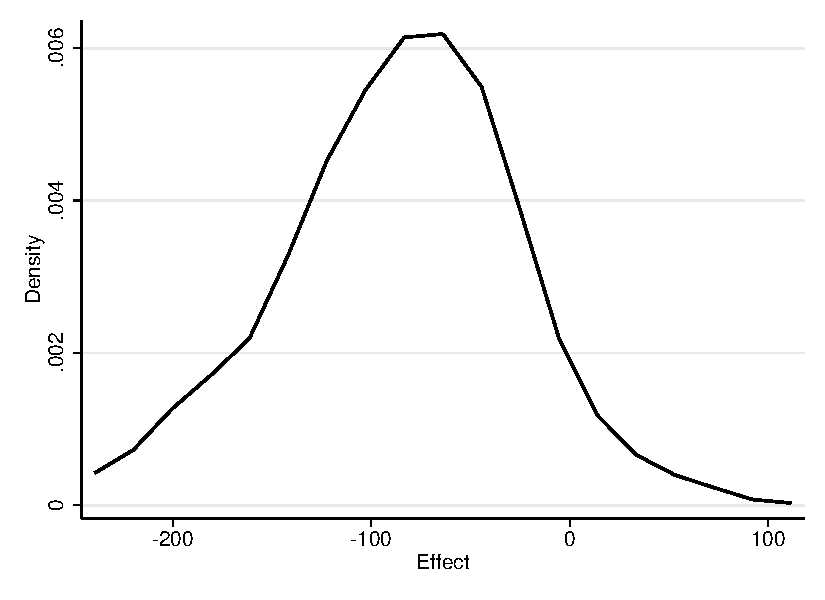
\includegraphics[width=\textwidth]{Figuras/he_dist_fc_admin_disc_pro_2.pdf}
%     %\end{subfigure}
%     \begin{subfigure}{0.7\textwidth}
%         \caption{Determinants of effects}
%         \centering
%         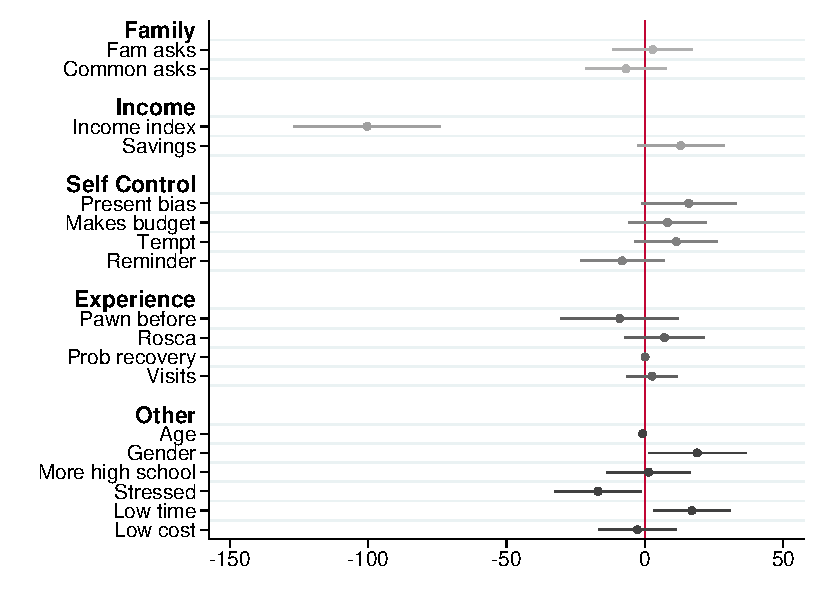
\includegraphics[width=\textwidth]{Figuras/HE/he_int_vertical_fc_admin_disc_pro_2.pdf}
%     \end{subfigure}
    
%     %\begin{subfigure}{0.4\textwidth}
%     %    \caption{Losing Pawn}
%     %    \centering
%     %    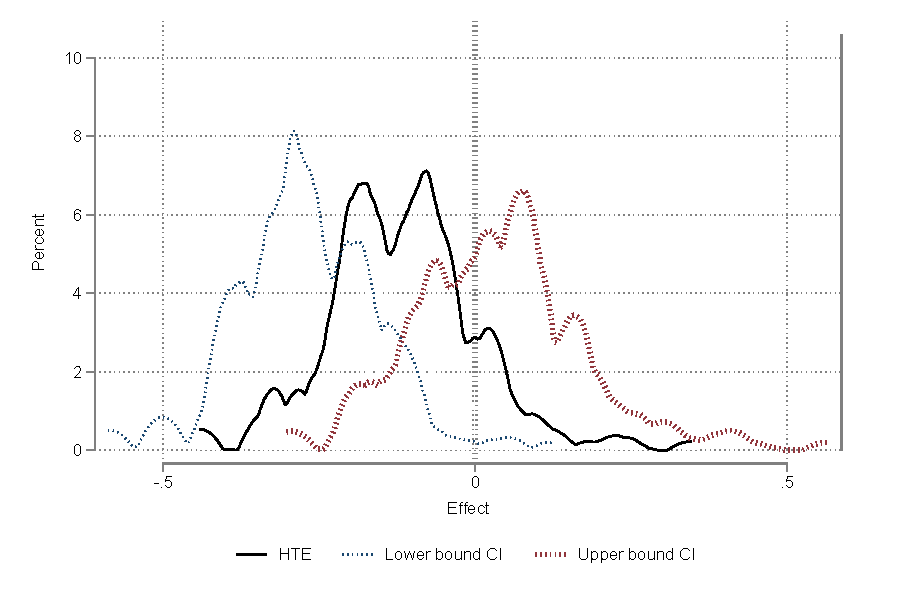
\includegraphics[width=\textwidth]{Figuras/he_dist_def_c_pro_2.pdf}
%     %\end{subfigure}
%     %\begin{subfigure}{0.4\textwidth}
%     %    \caption*{}
%     %    \centering
%     %    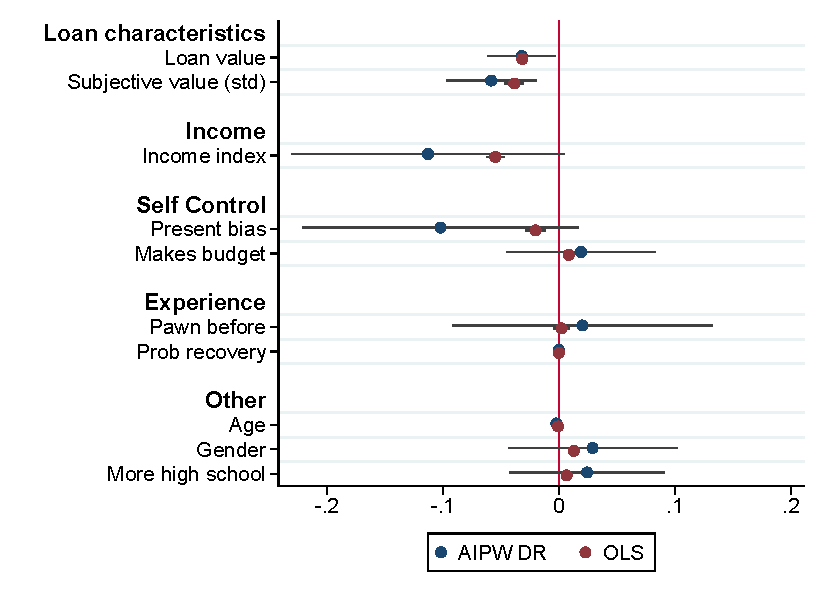
\includegraphics[width=\textwidth]{Figuras/HE/he_int_vertical_def_c_pro_2.pdf}
%     %\end{subfigure}
%     \end{center}
%      \scriptsize  This figure estimates bivariate regressions of the estimated client-level heterogeneous treatment effects against the respective covariate from the baseline survey  $\widehat{hte_i} = \alpha + \beta \: X_i + \epsilon_i$. The regressors $X_i$ include (e.g if the family asks for money, if they have savings, if they are overconfident using the definition the text, etc. See this Appendix for a transcription of the survey).
%       %\footnotesize{ \textit{Do file: }  \texttt{analyze\_grf\_single\_arm.do}}
% \end{figure}



\begin{comment}
\begin{figure}[H]
    \caption{Heterogeneous Treatment Effect: Promise-forcing contract}
    \label{heterogeneous_te_3}
    \begin{center}
    \begin{subfigure}{0.4\textwidth}
        \caption{Financial cost}
        \centering
        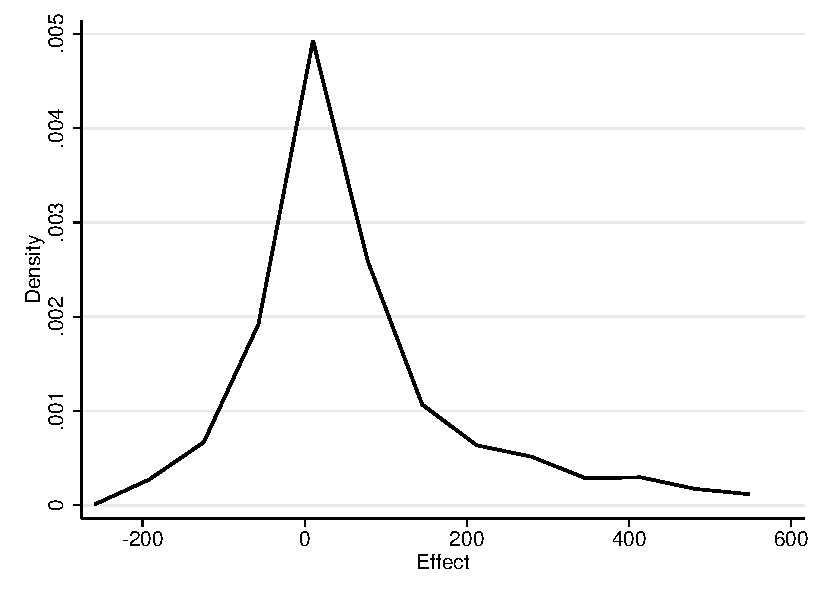
\includegraphics[width=\textwidth]{Figuras/he_dist_fc_admin_disc_pro_3.pdf}
    \end{subfigure}
    \begin{subfigure}{0.4\textwidth}
        \caption*{}
        \centering
        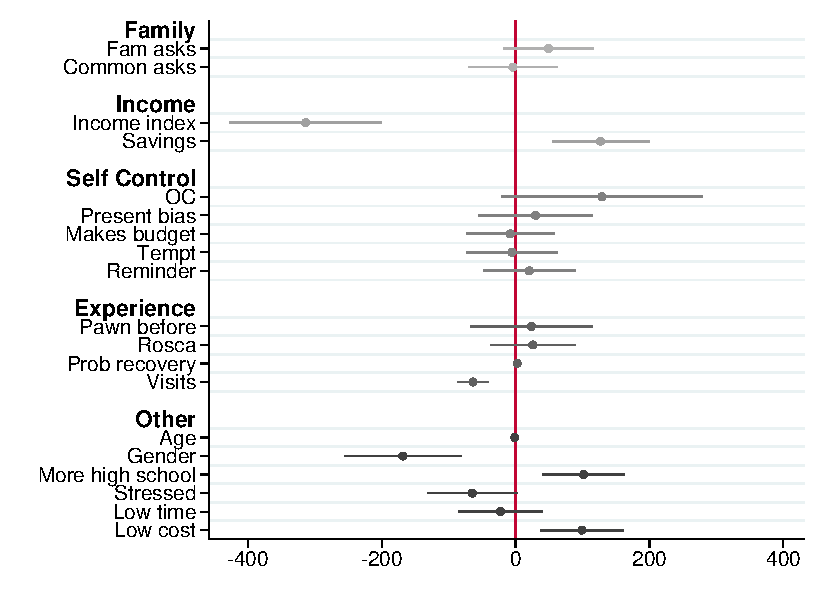
\includegraphics[width=\textwidth]{Figuras/HE/he_int_vertical_fc_admin_disc_pro_3.pdf}
    \end{subfigure}
    
    \begin{subfigure}{0.4\textwidth}
        \caption{Losing Pawn}
        \centering
        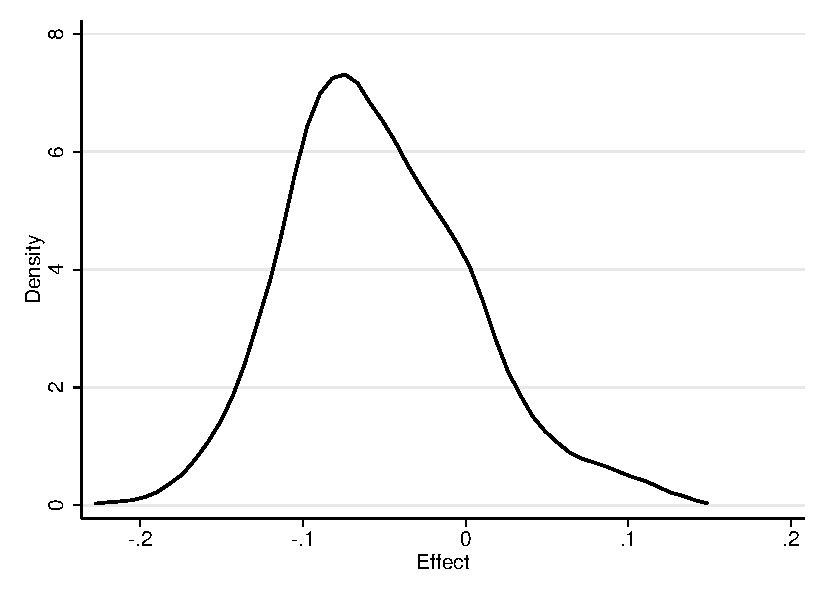
\includegraphics[width=\textwidth]{Figuras/he_dist_def_c_pro_3.pdf}
    \end{subfigure}
    \begin{subfigure}{0.4\textwidth}
        \caption*{}
        \centering
        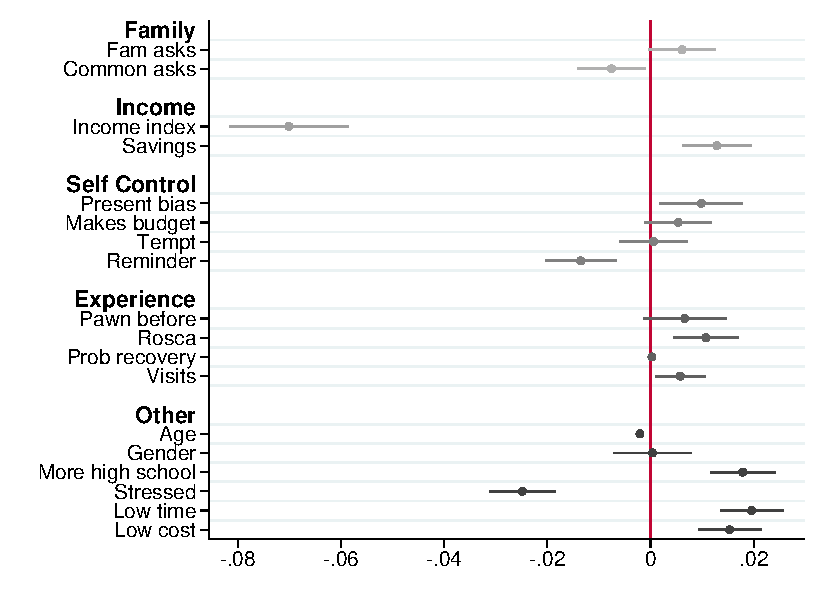
\includegraphics[width=\textwidth]{Figuras/HE/he_int_vertical_def_c_pro_3.pdf}
    \end{subfigure}
    \end{center}
     \scriptsize
      %\footnotesize{ \textit{Do file: }  \texttt{analyze\_grf\_single\_arm.do}}
\end{figure}
\end{comment}





\begin{comment}

\begin{figure}[H]
    \caption{Heterogeneous Treatment Effect - Choice/Fee}
    \label{heterogeneous_te_4}
    \begin{center}
    \begin{subfigure}{0.4\textwidth}
        \caption{Financial cost}
        \centering
        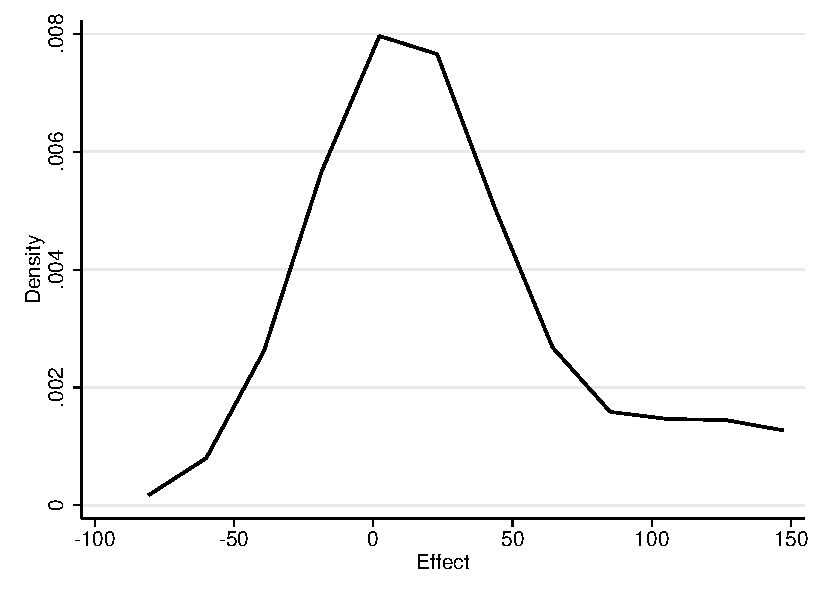
\includegraphics[width=\textwidth]{Figuras/he_dist_fc_admin_disc_pro_4.pdf}
    \end{subfigure}
    \begin{subfigure}{0.4\textwidth}
        \caption*{}
        \centering
        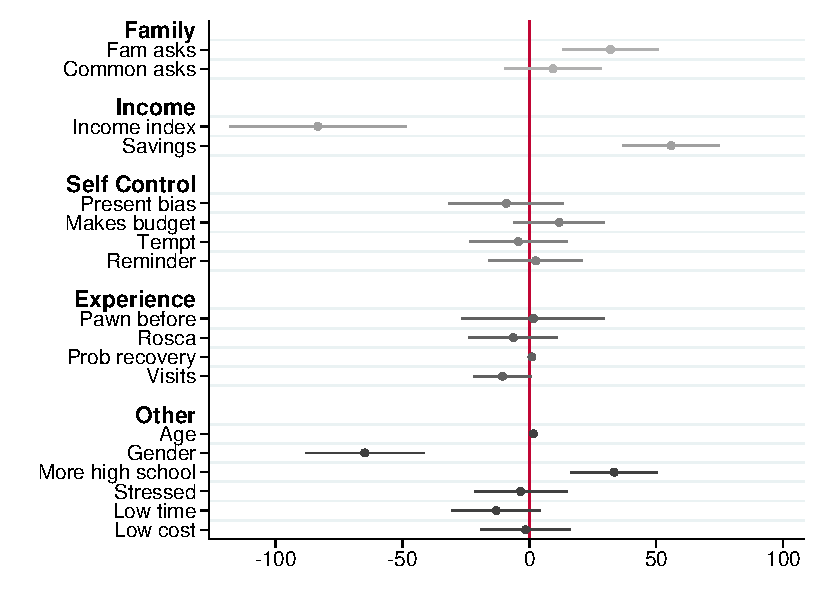
\includegraphics[width=\textwidth]{Figuras/HE/he_int_vertical_fc_admin_disc_pro_4.pdf}
    \end{subfigure}
    
    \begin{subfigure}{0.4\textwidth}
        \caption{Losing Pawn}
        \centering
        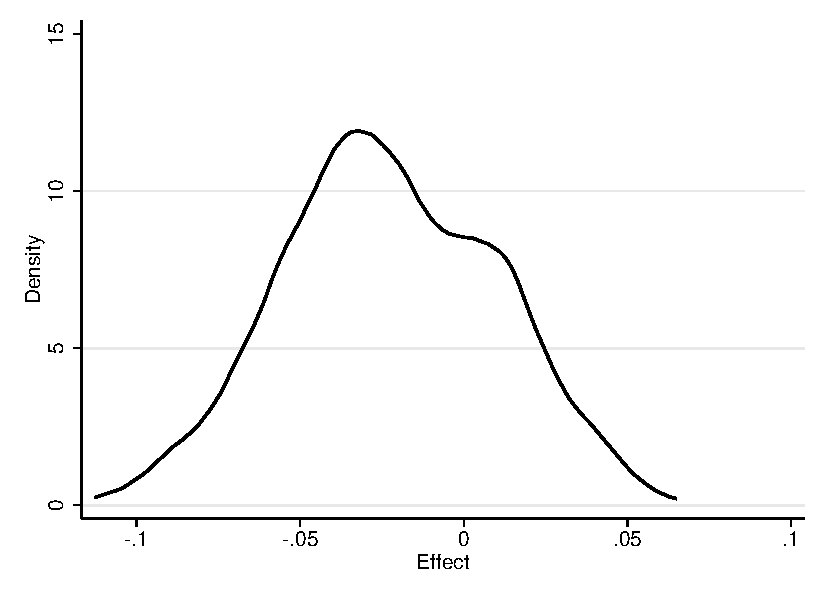
\includegraphics[width=\textwidth]{Figuras/he_dist_def_c_pro_4.pdf}
    \end{subfigure}
    \begin{subfigure}{0.4\textwidth}
        \caption*{}
        \centering
        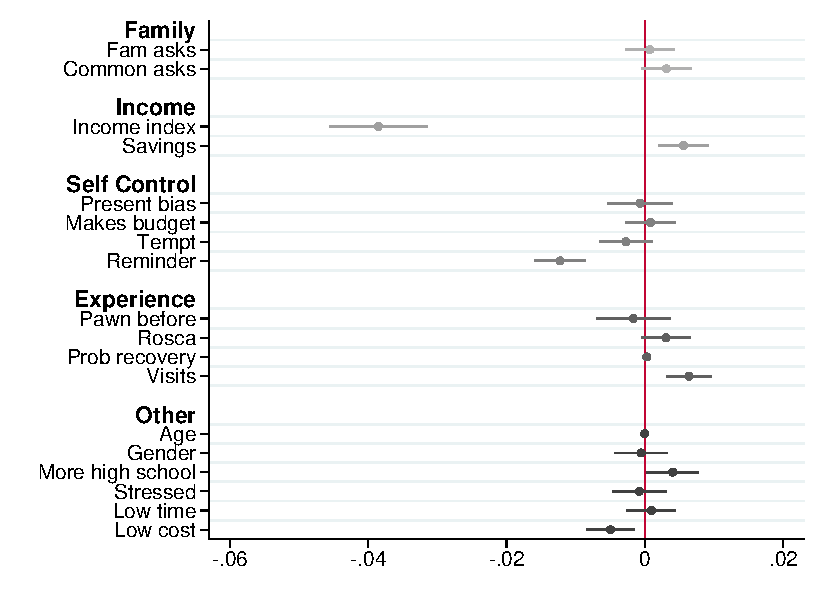
\includegraphics[width=\textwidth]{Figuras/HE/he_int_vertical_def_c_pro_4.pdf}
    \end{subfigure}
    \end{center}
     \footnotesize \textit{Notes: } The distribution plots the FC treatment effect for the interval $[\mu-2\sigma,\mu+2\sigma]$ to ignore the outliers.
      \footnotesize{ \textit{Do file: }  \texttt{analyze\_grf\_single\_arm.do}}
\end{figure}




\begin{figure}[H]
    \caption{Heterogeneous Treatment Effect - Choice/Promise}
    \label{heterogeneous_te_5}
    \begin{center}
    \begin{subfigure}{0.4\textwidth}
        \caption{Financial cost}
        \centering
        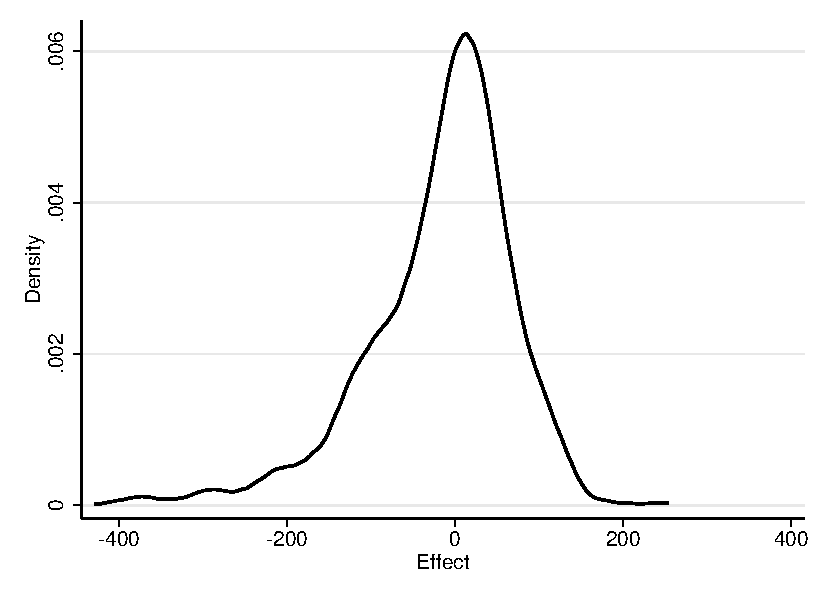
\includegraphics[width=\textwidth]{Figuras/he_dist_fc_admin_disc_pro_5.pdf}
    \end{subfigure}
    \begin{subfigure}{0.4\textwidth}
        \caption*{}
        \centering
        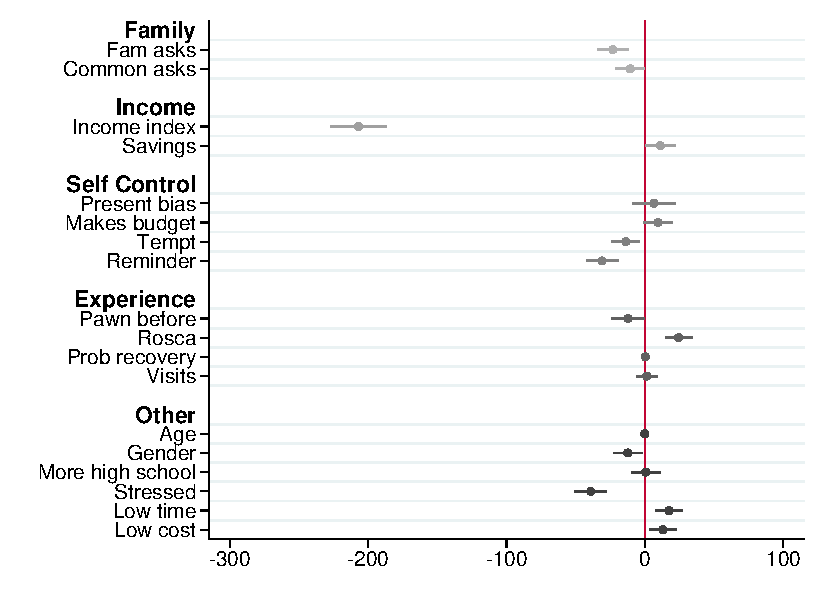
\includegraphics[width=\textwidth]{Figuras/HE/he_int_vertical_fc_admin_disc_pro_5.pdf}
    \end{subfigure}
    \begin{subfigure}{0.4\textwidth}
        \caption{Losing Pawn}
        \centering
        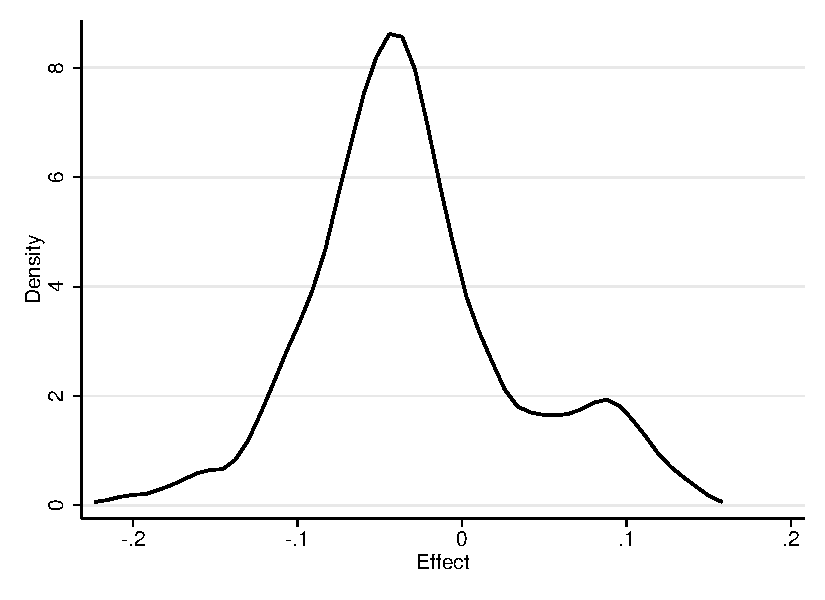
\includegraphics[width=\textwidth]{Figuras/he_dist_def_c_pro_5.pdf}
    \end{subfigure}
    \begin{subfigure}{0.4\textwidth}
        \caption*{}
        \centering
        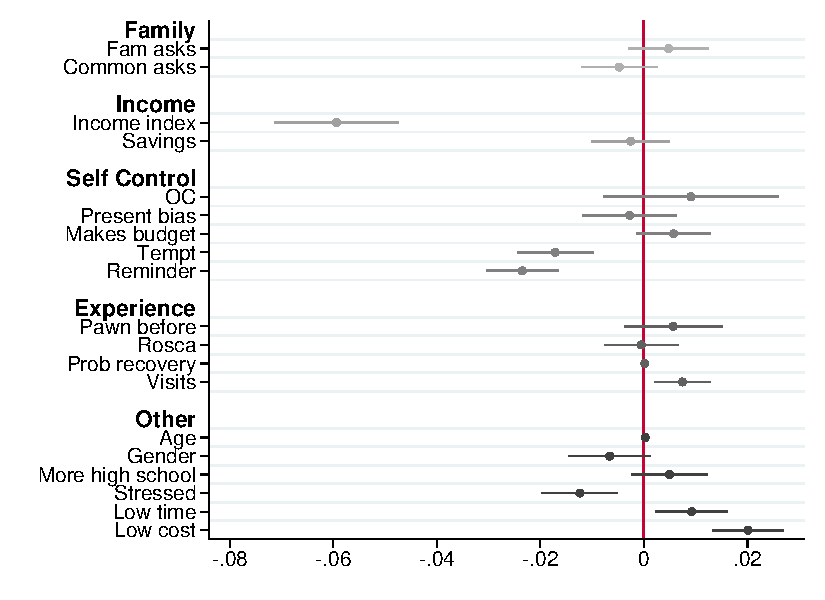
\includegraphics[width=\textwidth]{Figuras/HE/he_int_vertical_def_c_pro_5.pdf}
    \end{subfigure}
    \end{center}
     \footnotesize \textit{Notes: } 
      \footnotesize{ \textit{Do file: }  \texttt{analyze\_grf\_single\_arm.do}}
\end{figure}

\end{comment}







%\begin{figure}[H]
%    \caption{Heterogeneous Treatment Effect (FC survey) - All arms}
%    \label{heterogeneous_te_fcsurvey_all}
%    \begin{center}
%    \begin{subfigure}{0.4\textwidth}
%        \caption{Forcing/Fee}
%        \centering
%        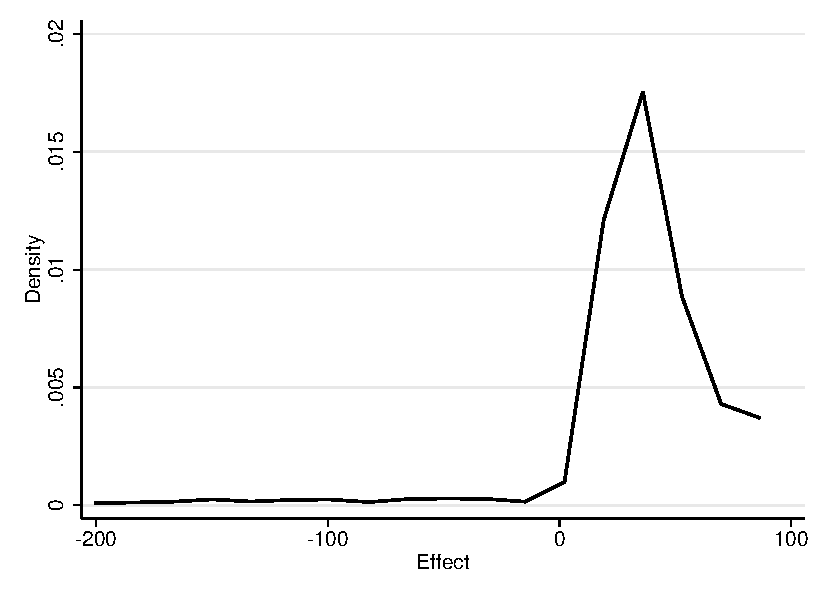
\includegraphics[width=\textwidth]{Figuras/he_dist_fc_survey_disc_pro_2.pdf}
%    \end{subfigure}
%    \begin{subfigure}{0.4\textwidth}
%        \caption{Forcing/Promise}
%        \centering
%        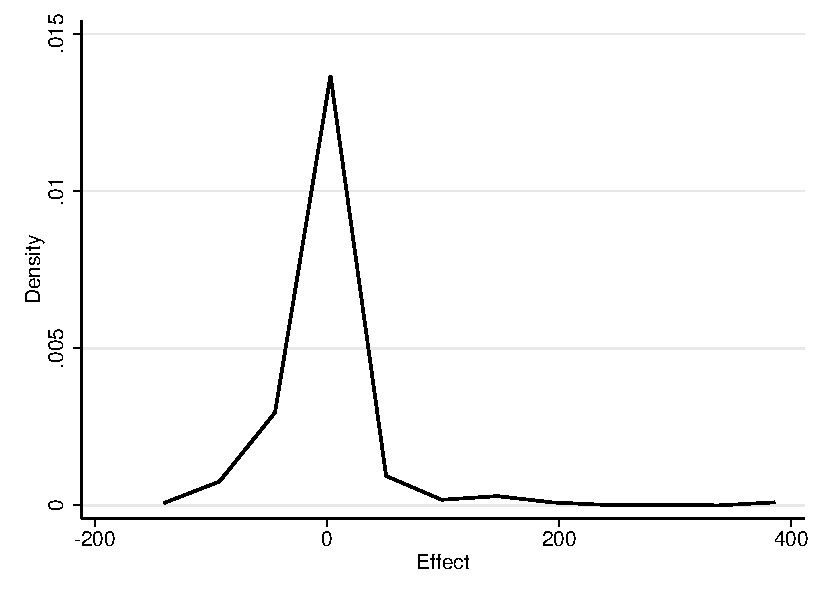
\includegraphics[width=\textwidth]{Figuras/he_dist_fc_survey_disc_pro_3.pdf}
%    \end{subfigure}
    
%    \begin{subfigure}{0.4\textwidth}
%        \caption{Choice/Fee}
%        \centering
%        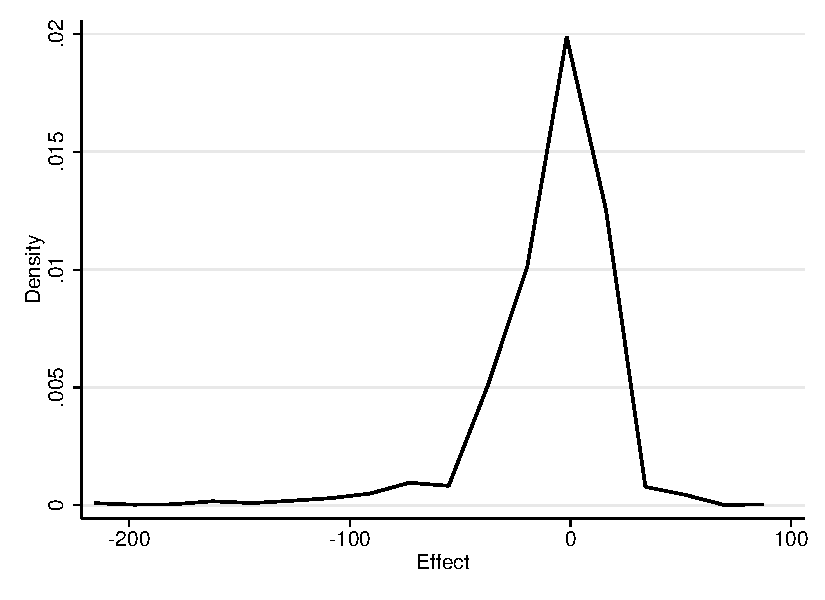
\includegraphics[width=\textwidth]{Figuras/he_dist_fc_survey_disc_pro_4.pdf}
%    \end{subfigure}
%    \begin{subfigure}{0.4\textwidth}
%        \caption{Choice/Promise}
%        \centering
%        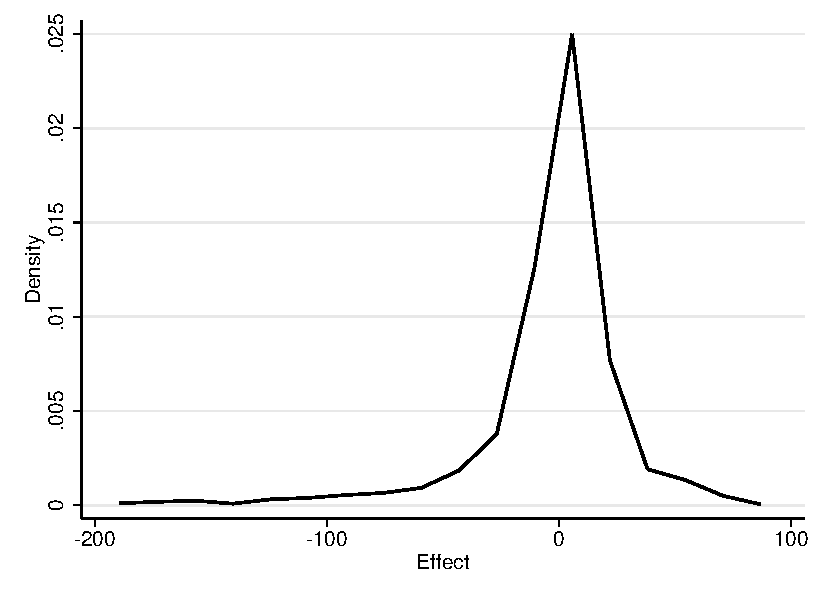
\includegraphics[width=\textwidth]{Figuras/he_dist_fc_survey_disc_pro_5.pdf}
%    \end{subfigure}
%    \end{center}
%     \footnotesize \textit{Notes: } 
%      \footnotesize{ \textit{Do file: }  \texttt{analyze\_grf\_single\_arm.do}}
%\end{figure}



\subsection{Take up}


\begin{table}[H]
    \caption{Predicting Take-up: Goodness-of-Fit}
    \label{Table_compliance}
    %\begin{subtable}{1\textwidth}
    % \centering
    %    \caption{Take up}
    %    \scriptsize{% Table generated by Excel2LaTeX from sheet 'oos_pago_frec_vol'
\begin{tabular}{lcccc}
\toprule
      & \multicolumn{4}{c}{Frequent voluntary payment } \\
\midrule
\midrule
OOS measures & Logit & SW-Logit & RF    & Boosting \\
\midrule
\midrule
MAE   & 0.32  & 0.33  & 0.33  & 0.29 \\
MSE   & 0.17  & 0.17  & 0.16  & 0.16 \\
AUC (out of sample) & 0.71  & 0.71  & 0.77  & 0.73 \\
      & (0.04) & (0.04) & (0.04) & (0.04) \\
AUC (in sample) & 0.77  & 0.76  & 0.88  & 0.96 \\
      & (0.02) & (0.02) & (0.01) & (0.01) \\
Accuracy & 0.7   & 0.7   & 0.75  & 0.77 \\
Correlation (0-1) & 0.21  & 0.22  & 0.39  & 0.38 \\
Correlation (predicted val) & 0.33  & 0.33  & 0.42  & 0.4 \\
R-squared  & 0.11  & 0.11  & 0.16  & 0.15 \\
Expected value of predictions & 0.25  & 0.25  & 0.24  & 0.22 \\
\bottomrule
\bottomrule
\end{tabular}%
}
    %\end{subtable}%
    
    %\bigskip
     \begin{subtable}{1\textwidth}
      \centering
        \caption{Take up: Choice-fee Arm}
        \scriptsize{% Table generated by Excel2LaTeX from sheet 'oos_pago_frec_vol_fee'
\begin{tabular}{lcccc}
\toprule
      & \multicolumn{4}{c}{Frequent voluntary payment - FEE} \\
\midrule
\midrule
OOS measures & Logit & SW-Logit & RF    & Boosting \\
\midrule
\midrule
MAE   & 0.21  & 0.21  & 0.23  & 0.17 \\
MSE   & 0.1   & 0.1   & 0.1   & 0.09 \\
AUC (out of sample) & 0.76  & 0.78  & 0.84  & 0.85 \\
      & (0.06) & (0.06) & (0.06) & (0.05) \\
AUC (in sample) & 0.84  & 0.82  & 0.92  & 0.99 \\
      & (0.02) & (0.02) & (0.01) & (0.01) \\
Accuracy & 0.82  & 0.84  & 0.86  & 0.88 \\
Correlation (0-1) & 0.13  & 0.26  & 0.37  & 0.31 \\
Correlation (predicted val) & 0.33  & 0.38  & 0.37  & 0.43 \\
R-squared  & 0.08  & 0.13  & 0.11  & 0.19 \\
Expected value of predictions & 0.17  & 0.17  & 0.16  & 0.12 \\
\bottomrule
\bottomrule
\end{tabular}%
}
    \end{subtable}
    
      \bigskip
    \begin{subtable}{1\textwidth}
      \centering
        \caption{Take up: Choice-promise Arm}
        \scriptsize{% Table generated by Excel2LaTeX from sheet 'oos_pago_frec_vol_promise'
\begin{tabular}{lcccc}
\toprule
      & \multicolumn{4}{c}{Frequent voluntary payment - PROMISE} \\
\midrule
\midrule
OOS measures & Logit & SW-Logit & RF    & Boosting \\
\midrule
\midrule
MAE   & 0.41  & 0.41  & 0.41  & 0.36 \\
MSE   & 0.24  & 0.23  & 0.21  & 0.21 \\
AUC (out of sample) & 0.63  & 0.63  & 0.7   & 0.72 \\
      & (0.06) & (0.06) & (0.06) & (0.06) \\
AUC (in sample) & 0.83  & 0.82  & 0.9   & 0.97 \\
      & (0.02) & (0.02) & (0.01) & (0.01) \\
Accuracy & 0.62  & 0.67  & 0.65  & 0.7 \\
Correlation (0-1) & 0.15  & 0.25  & 0.23  & 0.32 \\
Correlation (predicted val) & 0.22  & 0.21  & 0.3   & 0.35 \\
R-squared  & -0.06 & -0.05 & 0.08  & 0.08 \\
Expected value of predictions & 0.39  & 0.38  & 0.38  & 0.35 \\
\bottomrule
\bottomrule
\end{tabular}%
}
    \end{subtable}
            \scriptsize
           \\
           \\
           \\
    
     %\textit{Scripts: } \texttt{pred\_take\_up.do, pfv\_pred.R}
\end{table}




\vspace{.1in}
\begin{figure}[H]
    \caption{Out of sample ROC curve}
    \label{roc_curve}
    \begin{center}
    \begin{subfigure}{0.45\textwidth}
        \caption{Take-up in Fee Arm}
        \centering
        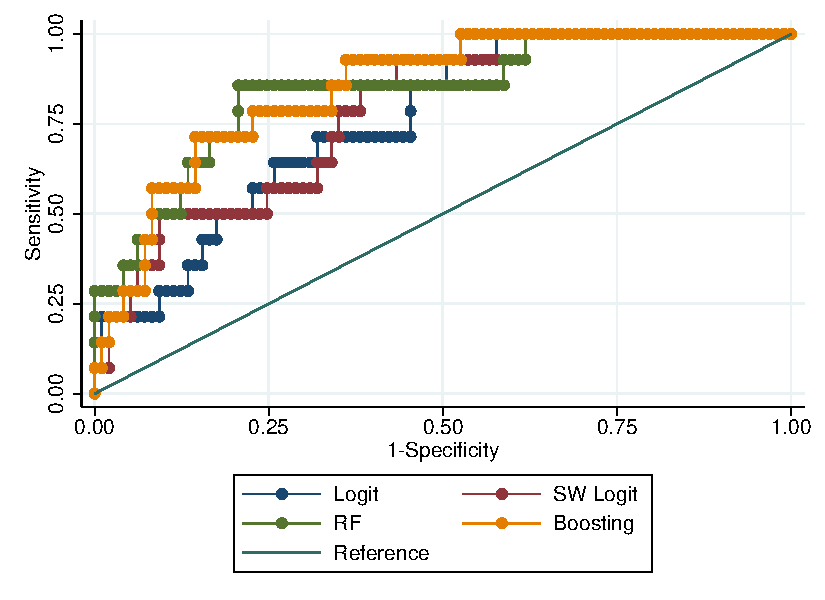
\includegraphics[width=\textwidth]{Figuras/Boost/ROC_curve_outsample_pago_frec_vol_fee.pdf}
    \end{subfigure}
    \begin{subfigure}{0.45\textwidth}
        \caption{Take-up in Promise Arm}
        \centering
        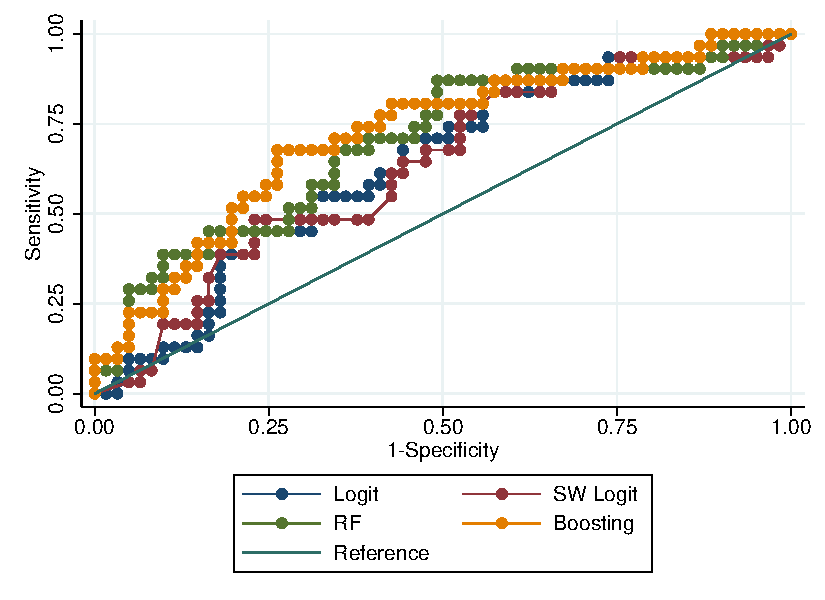
\includegraphics[width=\textwidth]{Figuras/Boost/ROC_curve_outsample_pago_frec_vol_promise.pdf}
    \end{subfigure}
    \end{center}
     \scriptsize 
  %\footnotesize{ \textit{Do file: }  \texttt{pred\_take\_up.do}}
\end{figure}



\begin{figure}[H]
    \caption{Predictors of commitment contract take-up}
    \label{interactions_takeup}
    \begin{center}
    \begin{subfigure}{0.45\textwidth}
        \caption{with Fee Arm}
        \centering
        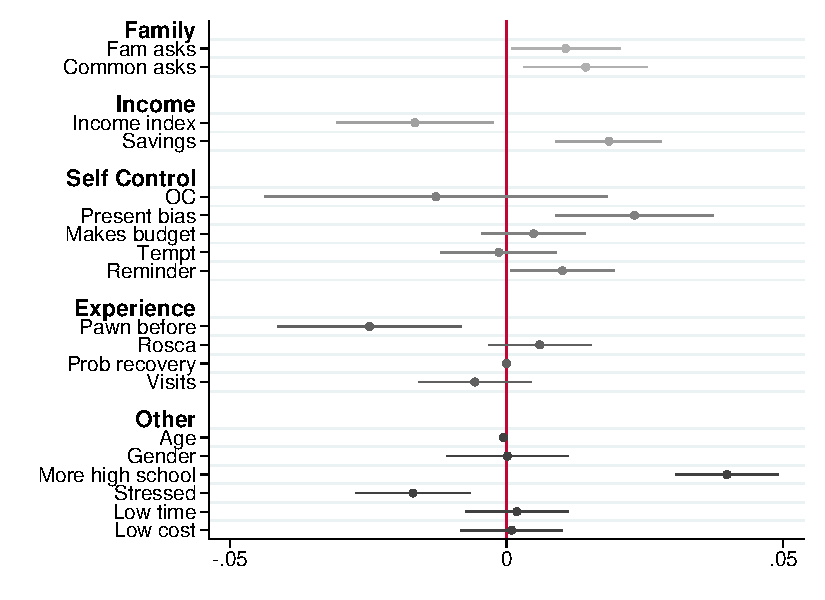
\includegraphics[width=\textwidth]{Figuras/pago_frec_vol_fee_interactions_rf.pdf}
    \end{subfigure}
    \begin{subfigure}{0.45\textwidth}
        \caption{with Promise Arm}
        \centering
        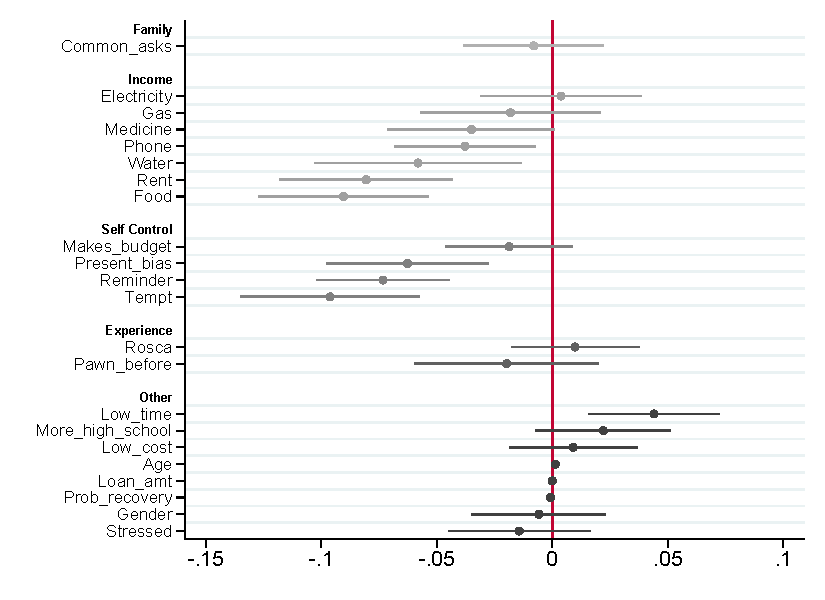
\includegraphics[width=\textwidth]{Figuras/pago_frec_vol_promise_interactions_rf.pdf}
    \end{subfigure}
    \end{center}
     \scriptsize
      %\footnotesize{ \textit{Do file: }  \texttt{analyze\_fvp.do}}
\end{figure}


\scriptsize {
\noindent This figure reports bivariate regressions of the form $\widehat{TakeUp} = \alpha + \beta \: X_i + \epsilon_i$, where $\widehat{TakeUp}$ is the prediction using random forests. The figure reports the $\beta$ coefficients for different $X_i$'s along with 95\% confidence intervals. Panel (a) focuses on take up in the arm where clients could chose among the fee-commitment contract and the status quo contract. Panel (b) focuses on the arm where clients could chose among the promise-commitment contract and the status quo contract. Using random forests we can predict who takes up the fee-forcing contract with 85\% accuracy out of sample.\footnote{Correcting for the fact that most chose the status-quo contract using the method of SMOTE, \cite{smote} we find an accuracy rate of 75\%.} Which suggests that choice among contracts is not purely random. This figure shows that the more educated, those that report that their family typically asks for money, those that make a monthly budget of expenses, and those that ask for a remainder of their due payments (and marginally those we classify as present-biased) are more likely to chose the fee-commitment contract if given the choice. The opposite holds for clients that are more economically vulnerable (can barely pay for food, electricity, etc) and those that report being more stressed.
}

\newpage

\subsection{Selection on gains}


\begin{figure}[H]
    \caption{Determinants of treatment effects and probability of choosing commitment}
    \label{determinants_ps_hte}
    \begin{center}
    \begin{subfigure}{0.475\textwidth}
        \caption{Determinants of HTE}
        \centering
        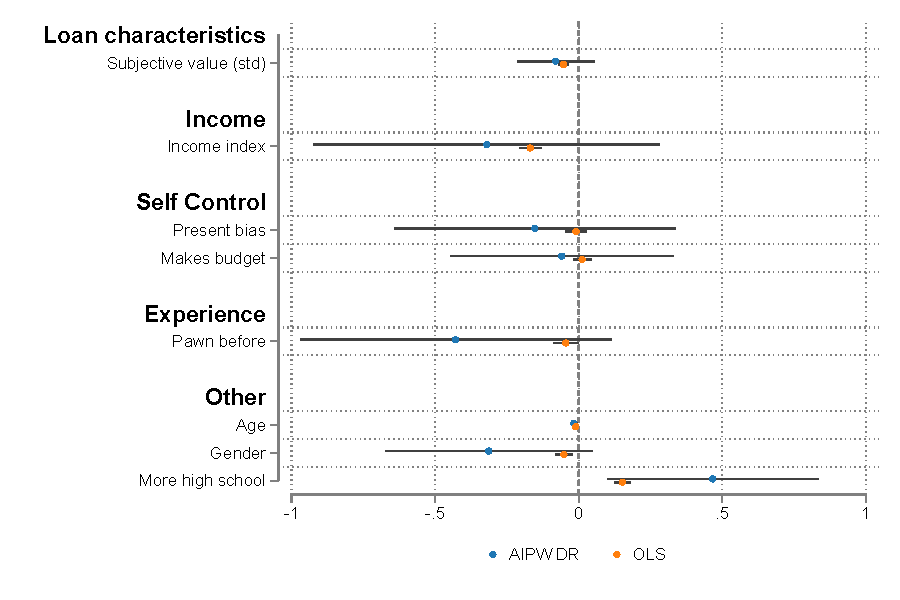
\includegraphics[width=\textwidth]{Figuras/HE/he_int_vertical_apr_pro_2.pdf}
    \end{subfigure}
    \begin{subfigure}{0.475\textwidth}
        \caption{Determinants of propensity score}
        \centering
        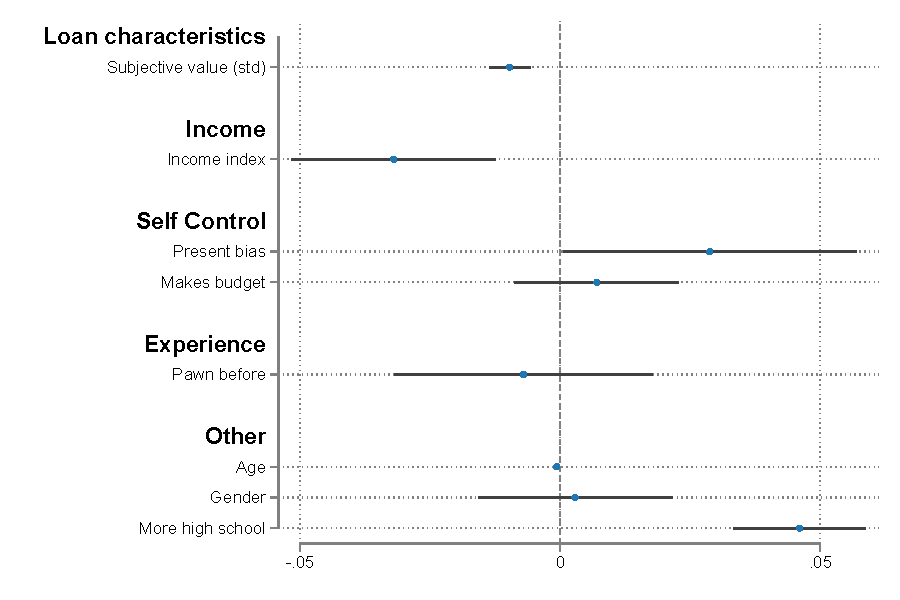
\includegraphics[width=\textwidth]{Figuras/HE/ps_int_vertical_pr_gbc_1.pdf}
    \end{subfigure}
  
    \end{center}
     \scriptsize   This figure estimates bivariate regressions of the estimated client-level (a) heterogeneous treatment effects, (b) propensity score, against the respective covariate from the baseline survey  $\widehat{HTE_i}, \widehat{P_i} = \alpha + \beta \: X_i + \epsilon_i$. The regressors $X_i$ include (e.g if the family asks for money, if they have savings, if they are overconfident using the definition the text, etc. See this Appendix for a transcription of the survey). \\
      %\footnotesize{ \textit{Do file: }  \texttt{analyze\_grf\_single\_arm.do}} \texttt{benefit\_choice.do}}
\end{figure}



\subsubsection{Finite mixture model }\label{fmm_section}

\vspace{.2in}
\normalsize
\linespread{1.25}

We assume the following structural model : Each individual $i$ is of type  $k\in\{1, 2\}$ with probability $\alpha_{i,k}$. We assume it follows a logit distribution:
\begin{align*}
\label{dist_alpha}
    \alpha_{i,k} = \Pr(\text{Type}_i = k \;|\; \mathbf{W}_{i}) = \frac{e^{\gamma_{k}\mathbf{W}_i}}{\sum_{j=1}^{K} e^{\gamma_{j}\mathbf{W}_i}}
\end{align*}

where $\mathbf{W}_i$ are observable characteristics. This characteristics include choice for commitment, present bias, subjective probability of recovery, etc, which might be indicators of naivete vs sophistication.  

Now, given their type, each individual makes a choice to default or not $c_{i,k} \in \{1,2\}$, based on other set of observable characteristics $\mathbf{X}_i$ (subjective \& objective value of the loan). We will assume there is a continuous latent variable $Y_{i,k,c}$ distributed as
\[Y_{i,k,c} = \beta_{c,k}\mathbf{X}_{i} +\epsilon_{c,k}\]
with\footnote{We can impose other errors, and even impose a covariance structure, for instance if $(\epsilon_{c,k})_{c}\sim\mathcal{N}(0,\Sigma_k)$, we arrive to the Multinomial Probit.} $\epsilon_{c;k}\sim\operatorname{EV}(0,1)$. This latent variable can be thought of as the utility associated with individual $i$, being type $k$, making choice $c$. 



Thus, the density for each individual $i$ being type $k$ is
\[f(c_i,\mathbf{X}_i; \bm\beta_{k}) = \prod_{c=1}^4\left(\frac{e^{\beta_{c,k} \mathbf{X}_i}}{\sum_{j=1}^{4} e^{\beta_{j,k}  \mathbf{X}_i}}\right)^{[c_i=4]}\]

Finally, the generative model is then a mixture model with density given by,
\begin{align*}
    f(c_i ,\mathbf{W}_i, \mathbf{X}_i; \bm{\gamma},\bm{\beta}) &= \sum_{k=1}^K \alpha_k f(c_i,\mathbf{X}_i; \bm\beta_{k}) \\
    &= \sum_{k=1}^K \alpha_k \prod_{c=1}^4\left(\frac{e^{\beta_{c,k} \mathbf{X}_i}}{\sum_{j=1}^{4} e^{\beta_{j,k}  \mathbf{X}_i}}\right)^{[c_i=c]} 
\end{align*}



where $\alpha\sim \operatorname{Categorical}$, and $\gamma_{K} = \beta_{4,k}=0$ for identification purposes. 

Then the (incomplete) log-likelihood function is
\begin{align*}
    \ell(\bm{\gamma}, \bm{\beta}; c, \mathbf{W},  \mathbf{X}) = \sum_{i=1}^n \log\sum_{k=1}^K \alpha_k \prod_{c=1}^4\left(\frac{e^{\beta_{c,k} \mathbf{X}_i}}{\sum_{j=1}^{4} e^{\beta_{j,k}  \mathbf{X}_i}}\right)^{[c_i=c]} 
\end{align*}

, thus we estimate parameters $(\bm{\gamma}, \bm{\beta})$ with an EM algorithm using choice (default), and observable characteristics: $(c_i,\mathbf{W}_i,\mathbf{X}_i)$.


\begin{table}[H]
\caption{FMM}
\label{fmm_table}
\begin{center}
\scriptsize{% Table generated by Excel2LaTeX from sheet 'fmm_types'
\begin{tabular}{lcc}
\cmidrule{1-2}      & Type 1 &  \\
\cmidrule{1-2}      & (1)   &  \\
\cmidrule{1-2}Demand commitment  & -1.73 &  \\
      & (0.76) &  \\
Income index & 3.92  &  \\
      & (3.28) &  \\
Present bias & 0.48  &  \\
      & (0.63) &  \\
Makes budget (almost always) & -1.11 &  \\
      & (0.71) &  \\
Makes budget (always) & 0.068 &  \\
      & (0.54) &  \\
Pawn before & -2.88 &  \\
      & (2.37) &  \\
Prob recovery & -0.011 &  \\
      & (0.014) &  \\
Age   & -0.031 &  \\
      & (0.023) &  \\
Gender & -0.34 &  \\
      & (0.45) &  \\
More than High-School & -1.00 &  \\
      & (0.76) &  \\
Constant & 6.72  &  \\
      & (3.19) &  \\
\cmidrule{1-2}      &       &  \\
      &       &  \\
\midrule
      & \multicolumn{2}{c}{Default} \\
\midrule
      & Type 1 & Type 2 \\
\midrule
\midrule
Loan value (log) & -0.95 & 4.23 \\
      & (0.47) & (1.67) \\
Subjective value & 0.00012 & -0.00080 \\
      & (0.000082) & (0.00035) \\
Constant  & 7.32  & -29.4 \\
      & (3.37) & (11.5) \\
      &       &  \\
\midrule
Observations & 786   & 786 \\
\midrule
Default \% (lower bound) & 0.58  & 0.19 \\
Default \%  & 0.70  & 0.3 \\
Default \% (upper bound) & 0.81  & 0.42 \\
\bottomrule
\bottomrule
\end{tabular}%
}
\end{center}
 \scriptsize

%\textit{Do file: } \texttt{fmm.do}
\end{table}


\begin{figure}[H]
    \caption{Treatment effect of Type 1 individuals}
    \label{fmm_hte}
    \begin{center}
    \begin{subfigure}{0.475\textwidth}       
            \caption{Probability of Type 1 vs HTE}
            \centering
        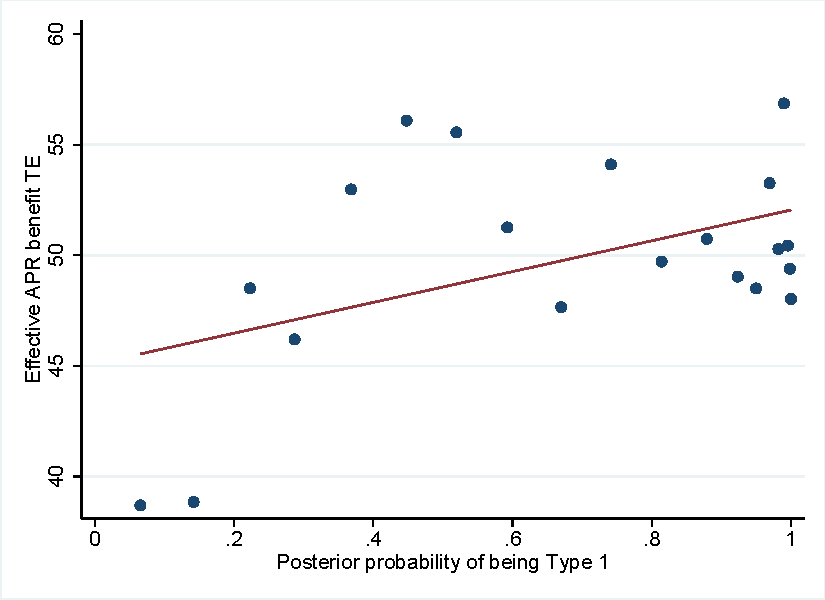
\includegraphics[width=\textwidth]{Figuras/binscatter_tau_classpost.pdf}
    \end{subfigure}
   \begin{subfigure}{0.475\textwidth}
        \caption{Type 1 vs HTE}
        \centering
        \includegraphics[width=\textwidth]{Figuras/benefit_type1p.pdf}
    \end{subfigure}
    \end{center}
     \scriptsize 
     After estimating the FMM, we compute the probability for each individual of belonging to each class, the x-axis represents the probability of being Type $1$, while the y-axis shows the HTE. A positive relation indicates that Type $1$ individuals are more benefited from commitment.
      %\footnotesize{ \textit{Do file: }  \texttt{fmm.do}} 
\end{figure}

\subsubsection{LATE: ToT \& TuT}
\vspace{.2in}
\normalsize
\linespread{1.25}


 Recall that $Z_i$ is the observed, randomly assigned experimental allocation, where $Z_i=0$ denotes the control arm, $Z_i=1$ denotes the forced-fee arm, and $Z_i=2$ is the choice arm.  Let $C_i$ be the unobserved choice type. $C_i=0$ when individual $i$ does not choose commitment  given the choice and $C_i=1$ when chooses commitment given the choice. Finally, $D_i = Z_i\times \mathds{1}(Z_i\neq 2) + T_i\times \mathds{1}(Z_i=2)$ is the observed treatment indicator, and $Y(d,z)$ is the potential outcome function for $d=0,1$, and $z=0,1,2$. 

 To identify assortative selection we first need to estimate the following quantities: $\mathbb{E}(Y_1-Y_0\;|\;C=1)$ the Treatment on the Treated (ToT), and $\mathbb{E}(Y_1-Y_0\;|\;C=0)$ the Treatment on the Untreated (TuT). 

 To point identify the above quantities, we make the following assumptions.

 \begin{assumption}[Exclusion Restriction]
$Z$ only affects $Y$ through its effect on $D$ : $C(d,z) = C(d)$
 \end{assumption}

  \begin{assumption}[Independence Assumption]
$Z \perp (Y_0, Y_1, C)$
 \end{assumption}

The following intermediate Lemmas will help us derive that both ToT and TuT are point identified.

\begin{lem}
$\Pr(C=1) = \E[D\;|\;Z=2]$
\end{lem}
\begin{proof}
Since $C\perp Z$, 
$$\E[D\;|\;Z=2] = \E[Z\times \mathds{1}(Z\neq 2)+ C\times\mathds{1}(Z=2)\;|Z=2] = \E[C\;|\;Z=2] = \E[C] = \Pr(C=1)$$
\end{proof}


\begin{lem}
$\E[Y_0] = \E[Y\;|\;Z=0]$
\end{lem}
\begin{proof}
Since $Z\perp Y_0$, 
\begin{align*}
\E[Y\;|\;Z=0] =& \E[\mathds{1}(Z=0)Y_0+\mathds{1}(Z=1)Y_1+\mathds{1}(Z=2)\{(1-C)Y_0+CY_1\})\;|\;Z=0]\\   
=&\E[Y_0\;|\;Z=0] = \E[Y_0]
\end{align*}
\end{proof}


\begin{lem}
$\E[Y_1] = \E[Y\;|\;Z=1]$
\end{lem}
\begin{proof}
Since $Z\perp Y_1$, 
\begin{align*}
\E[Y\;|\;Z=1] =\E[Y_1\;|\;Z=1] = \E[Y_1]
\end{align*}
\end{proof}


\begin{lem}
$\E[Y_0\;|\;C=0] = \E[Y\;|\; D=0,Z=2]$
\end{lem}
\begin{proof}
If $Z=2$, then $D=0$ if and only if $C=0$. Hence,
\[\E[Y\;|\;D=0, Z=2] = \E[Y_0\;|\;D=0, Z=2] = E[Y_0\;|\;C=0, Z=2]=\E[Y_0\;|\;C=0]\]
since $Y_0\perp C\;|\;Z$
\end{proof}

\begin{lem}
$\E[Y_1\;|\;C=1] = \E[Y\;|\; D=1,Z=2]$
\end{lem}
\begin{proof}
If $Z=2$, then $D=1$ if and only if $C=1$. Hence,
\[\E[Y\;|\;D=1, Z=2] = \E[Y_1\;|\;D=1, Z=2] = E[Y_1\;|\;C=1, Z=2]=\E[Y_1\;|\;C=1]\]
since $Y_1\perp C\;|\;Z$
\end{proof}

\begin{theorem} $\E[Y_1-Y_0\;|\; C=1]$ is point identified
\end{theorem}

\begin{proof}
Since $\E[Y_1\;|\; C=1] = \E[Y\;|\; D=1, Z=2]$ by Lemma 5, it suffices to show that $\E[Y_1\;|\;C=0]$ is point identified. By iterated expectations:
\[E[Y_0] = \E_C\E[Y_0\;|\;C] = (1-p)\E[Y_0\;|\;C=0]+p\E[Y_0\;|\;C=1]\]
where $p:=\E[C]=\Pr(C=1)$, and re-arranging,
\[\E[Y_0\;|\;C=1] = \frac{1}{p}\left(E[Y_0] -(1-p)\E[Y_0\;|\;C=0]\right)\]
Finally, substituting the result of Lemmas 1, 2, and 4, we obtain
\[\E[Y_0\;|\;C=1] =\frac{1}{\E[D\;|\;Z=2]}\left\{\E[Y\;|\;Z=0]-(1-\E[D\;|\;Z=2])\E[Y\;|\;D=0, Z=2]\right\}\]
and the RHS is a function of observed data only.
\end{proof}

\begin{theorem} $\E[Y_1-Y_0\;|\; C=0]$ is point identified
\end{theorem}

\begin{proof}
Since $\E[Y_0\;|\; C=0] = \E[Y\;|\; D=0, Z=2]$ by Lemma 4, it suffices to show that $\E[Y_0\;|\;C=1]$ is point identified. By iterated expectations:
\[E[Y_1] = \E_C\E[Y_1\;|\;C] = (1-p)\E[Y_1\;|\;C=0]+p\E[Y_1\;|\;C=1]\]
where $p:=\E[C]=\Pr(C=1)$, and re-arranging,
\[\E[Y_1\;|\;C=0] = \frac{1}{1-p}\left(E[Y_1] -p\E[Y_1\;|\;C=1]\right)\]
Finally, substituting the result of Lemmas 1, 3, and 5, we obtain
\[\E[Y_1\;|\;C=0] =\frac{1}{1-\E[D\;|\;Z=2]}\left\{\E[Y\;|\;Z=1]-\E[D\;|\;Z=2]\E[Y\;|\;D=1, Z=2]\right\}\]
and the RHS is a function of observed data only.
\end{proof}


\begin{figure}[H]
    \caption{Bootstrap inference for the difference between ToT-TuT}
    \label{bootstrap_tot_tut}
    \begin{center}
    \begin{subfigure}{0.31\textwidth}
        \caption{Simple}
        \centering
        \includegraphics[width=\textwidth]{Figuras/tot_tut_btsp1.pdf}
    \end{subfigure}
    \begin{subfigure}{0.31\textwidth}
        \caption{Admin controls}
        \centering
        \includegraphics[width=\textwidth]{Figuras/tot_tut_btsp2.pdf}
    \end{subfigure}
    \begin{subfigure}{0.31\textwidth}
        \caption{Admin + Survey controls}
        \centering
        \includegraphics[width=\textwidth]{Figuras/tot_tut_btsp3.pdf}
    \end{subfigure}
  
    \end{center}
     \scriptsize  Given that all of the arms are effectively randomly sampled form the same pool, we can also estimate the ToT and TuT with the pooled regression: $Y_i = \beta_0\mathds{1}(Z_i=0)+\beta_1\mathds{1}(Z_i=1)+\beta_2\mathds{1}(Z_i=2)+ \epsilon_i$, and then this test statistic just becomes the F-test on $\frac{\widehat{\beta_2}-\widehat{\beta_0}}{p}$ for the ToT, $\frac{\widehat{\beta_1}-\widehat{\beta_2}}{1-p}$ for the TuT, and an F-test on the difference between these two quantities to test whether the gains are different between compliers and non-compliers. Recognizing the stochastic nature of the compliance rate, we also bootstrap this quantity before running the previous regression. The red line shows the point estimate for the difference between ToT-TuT, and the gray bar in the x-axis shows a 95\% confidence interval for this difference. Panel (a) shows the difference between the ToT and TuT without any controls, while panel (b) and (c) adds admin controls and admin + survey controls respectively.
          %\footnotesize{ \textit{Do file: }  \texttt{tot\_tut.do}}
\end{figure}


\begin{figure}[H]
     \caption{ToT-TuT CDF}
     \label{tot_tut_ecdf}
    \begin{center}
    \begin{subfigure}{0.6\textwidth}
        \centering
        \includegraphics[width=\textwidth]{Figuras/cdf_tot_tut.pdf}
    \end{subfigure}
    \end{center}
    \scriptsize
       Equipped with estimates for the ToT and TuT for each individual $i$ from an Instrumental Random Forest we compute the ECDF for this quantities. The solid line is the ECDF for the ToT, the dashed line is the ECDF for the TuT, and the dotted line plots the difference between the ToT and the TuT - the blue dashed line in the x-axis shows the points where this difference is significant. The bold black interval at the bottom of the graph is the mean for the ToT distribution (0.07), while the gray interval shows the mean for the TuT distribution (0.10).
       
          %\footnotesize{ \textit{Do file: }  \texttt{tot\_tut\_insforest.do}}
\end{figure}

\begin{figure}[H]
     \caption{Exclusion restriction}
     \label{exclusion_restriction}
    \begin{center}
    \begin{subfigure}{0.6\textwidth}
        \centering
        \includegraphics[width=\textwidth]{Figuras/exclusion_restriction.pdf}
    \end{subfigure}
    \end{center}
    \scriptsize This figure serves as a test for the exclusion restriction in the point identification for the ToT and the TuT. It shows the effect on the effective cost/loan ratio for the forced-fee arm and the choice arm, together with the decomposition of the choosers and non-choosers. Note that a) being forced into the treatment (Forced fee) has the same effect as choosing it (Choosers), and b) not choosing the treatment (Non chooser) has no effect with respect to the control.
    
          %\footnotesize{ \textit{Do file: }  \texttt{exclusion\_restriction.do}}
\end{figure}

%---------------------------------------------------------------------------------------------------------------------------------------------------------------------------------------------------------------------------------

\newpage 

\subsection{New results}
\begin{figure}[H]
        \caption{Financial cost for different discount rates}
    \label{fc_discount_rates}
    \begin{center}
        \centering
        \includegraphics[width=0.55\textwidth]{Figuras/discount_effect.pdf}
    \end{center}
     \scriptsize This Figure estimates the treatment effect on financial cost with different discount rates.  
     %\textit{Do file: }  \texttt{discounted\_noeffect.do}
\end{figure}



% \begin{figure}[H]
%     \caption{Treatment effects pooling all arms}
%     \label{pooled_arms_te}
%     \begin{center}
%     \begin{subfigure}{0.45\textwidth}
%         \caption{Financial Cost}
%         \centering
%         \includegraphics[width=\textwidth]{Figuras/te_allarms_fc_admin_disc.pdf}
%     \end{subfigure}
%     \begin{subfigure}{0.45\textwidth}
%         \caption{Lost Pawn}
%         \centering
%         \includegraphics[width=\textwidth]{Figuras/te_allarms_def_c.pdf}
%     \end{subfigure}
%     \end{center}
%      \scriptsize
%       %\footnotesize{ \textit{Do file: }  \texttt{te\_allarms.do}}
% \end{figure}


\scriptsize {
\noindent This Figure shows the treatment effects for the main outcomes when pooling all arms in the same regression.
}

\begin{figure}[H]
        \caption{Treatment effect decomposition of the Financial Cost }
    \label{reg_int_pro_2}
    \begin{center}
        \centering
        \includegraphics[width=0.60\textwidth]{Figuras/int_te_pro_2.pdf}
    \end{center}
     \scriptsize This Figure is a "close-up" for the estimates found in Figure \ref{fc_pro2} - Panel (a). It shows the treatment effects on payed \& incurred interest, the former defined as the actual interest payed, and the latter is the sum of all potential interests (for those pawns that were lost we calculate the interest generated until day 230). In the right axis we show the treatment effect on the payed fees. Finally, we analyze this effect for the subsamples that recovers or loses the pawn.
     %\textit{Do file: }  \texttt{reg_\int.do}
\end{figure}


% \begin{figure}[H]
%         \caption{Frequency of renewals}
%     \label{ref_dist}
%     \begin{center}
%         \centering
%         \includegraphics[width=0.60\textwidth]{Figuras/ref_dist.pdf}
%     \end{center}
%      \scriptsize  This Figure shows the occurrence and frequency of renewals. It locates in time, respective to the day the loan started, when the renewal occurs for both the first and second renewal. Note that the first renewal is concentrated around 100 days, while the second is concentrated around the 200 days, corresponding to the first and second cycle. 
%      %\textit{Do file: }  \texttt{ref_\dist.do}
% \end{figure}

\begin{figure}[H]
    \caption{Histogram of payments}
    \label{hist_payments}
    \begin{center}
    \begin{subfigure}{0.31\textwidth}
        \caption{Status-quo}
        \centering
        \includegraphics[width=\textwidth]{Figuras/hist_payments_sq.pdf}
    \end{subfigure}
    \begin{subfigure}{0.31\textwidth}
        \caption{Forced commitment}
        \centering
        \includegraphics[width=\textwidth]{Figuras/hist_payments_fc.pdf}
    \end{subfigure}
    \begin{subfigure}{0.31\textwidth}
        \caption{Choice commitment}
        \centering
        \includegraphics[width=\textwidth]{Figuras/hist_payments_cc.pdf}
    \end{subfigure}    
        \begin{subfigure}{0.31\textwidth}
        \caption{Forced soft}
        \centering
        \includegraphics[width=\textwidth]{Figuras/hist_payments_fs.pdf}
    \end{subfigure}
    \begin{subfigure}{0.31\textwidth}
        \caption{Choice soft}
        \centering
        \includegraphics[width=\textwidth]{Figuras/hist_payments_cs.pdf}
    \end{subfigure} 
    \end{center}
     \scriptsize
      %\footnotesize{ \textit{Do file: }  \texttt{hist\_payments.do}}
\end{figure}


\begin{figure}[H]
        \caption{Survival graphs}
    \label{survival_graph}
    \begin{center}
   \begin{subfigure}{0.45\textwidth}
        \caption{Closed contracts}
        \centering
        \includegraphics[width=\textwidth]{Figuras/survival_graph_ended.pdf}
    \end{subfigure} 
       \begin{subfigure}{0.45\textwidth}
        \caption{Recovery}
        \centering
        \includegraphics[width=\textwidth]{Figuras/survival_graph_unpledge.pdf}
    \end{subfigure} 
    \end{center}
     \scriptsize  This Figure shows the accumulated percentage of recovery in time by treatment arm. 
     %\textit{Do file: }  \texttt{survival\_graph.do}
\end{figure}





%\begin{figure}[H]
%    \caption{Exit Survey: reasons to pawn or not again with monthly payments}
%    \label{reasons}
%    \begin{center}
%    \begin{subfigure}{0.5\textwidth}
%        \caption{Pawn again because:}
%        \centering
%        \includegraphics[width=\textwidth]{Figuras/razones_si.pdf}
%    \end{subfigure}
%    \begin{subfigure}{0.5\textwidth}
%        \caption{Not pawn because:}
%        \centering
%        \includegraphics[width=\textwidth]{Figuras/razones_no.pdf}
%    \end{subfigure}
%    \end{center}
%     \footnotesize \textit{Notes: } 
%      \footnotesize{ \textit{Do file: }  \texttt{ss.do}}
%\end{figure}





%\begin{figure}[H]
%    \caption{Decomposition of the mistakes by `Overconfidence' for Promise Arms}
%    \label{Promise_errors}
%    \begin{center}
%    \begin{subfigure}{0.6\textwidth}
%        \caption{Promise}
%        \centering
%        \includegraphics[width=\textwidth]{Figuras/line_cw_fc_te_cf_OC_promise.pdf}
%    \end{subfigure}
%    \end{center}
%     \footnotesize 
%     \textit{Notes: }  Decomposition of the percentage of mistakes by overconfidence. 
%       \textit{Do file: }  \texttt{choose\_wrong\_quant\_wrong\_decomposition.do}
%\end{figure}


%\begin{figure}[H]
%        \caption{Types of agents that incur in different FC}
%    \label{components_fc}
%    \begin{center}
%        \centering
%        \includegraphics[width=\textwidth]{Figuras/scatter_fc_pay.pdf}
%    \end{center}
%     \footnotesize \textit{Notes: } 
%      \footnotesize{ \textit{Do file: }  \texttt{hist\_fc.do}}
%\end{figure}



\begin{comment}
\begin{figure}[H]
        \caption{Percentage of payments}
    \label{perc_payments}
    \begin{center}
    \begin{subfigure}{.31\textwidth}
    \caption{Control}
        \centering
        \includegraphics[width=\textwidth]{Figuras/hist_porc_pay_pro_1.pdf}
    \end{subfigure}
    \begin{subfigure}{.31\textwidth}
    \caption{Forcing - fee}
        \centering
        \includegraphics[width=\textwidth]{Figuras/hist_porc_pay_pro_2.pdf}
    \end{subfigure}   
     \begin{subfigure}{.31\textwidth}
    \caption{Forcing - promise}
        \centering
        \includegraphics[width=\textwidth]{Figuras/hist_porc_pay_pro_3.pdf}
    \end{subfigure}  
     \begin{subfigure}{.31\textwidth}
    \caption{Choice - fee}
        \centering
        \includegraphics[width=\textwidth]{Figuras/hist_porc_pay_pro_4.pdf}
    \end{subfigure}  
     \begin{subfigure}{.31\textwidth}
    \caption{Choice - fee - SQ}
        \centering
        \includegraphics[width=\textwidth]{Figuras/hist_porc_pay_pro_6.pdf}
    \end{subfigure}    
     \begin{subfigure}{.31\textwidth}
    \caption{Choice - fee - NSQ}
        \centering
        \includegraphics[width=\textwidth]{Figuras/hist_porc_pay_pro_7.pdf}
    \end{subfigure}    
     \begin{subfigure}{.31\textwidth}
    \caption{Choice - promise}
        \centering
        \includegraphics[width=\textwidth]{Figuras/hist_porc_pay_pro_5.pdf}
    \end{subfigure}  
     \begin{subfigure}{.31\textwidth}
    \caption{Choice - promise - SQ}
        \centering
        \includegraphics[width=\textwidth]{Figuras/hist_porc_pay_pro_8.pdf}
    \end{subfigure}    
     \begin{subfigure}{.31\textwidth}
    \caption{Choice - promise - NSQ}
        \centering
        \includegraphics[width=\textwidth]{Figuras/hist_porc_pay_pro_9.pdf}    
    \end{subfigure}        
    \end{center}
     \footnotesize \textit{Notes: } 
      \footnotesize{ \textit{Do file: }  \texttt{hist\_payments.do}}
\end{figure}




\begin{figure}[H]
        \caption{Percentage of payment conditional on positive payment and Losing Pawn}
    \label{perc_payments_conditional}
    \begin{center}
    \begin{subfigure}{.31\textwidth}
    \caption{Control}
        \centering
        \includegraphics[width=\textwidth]{Figuras/hist_porc_pay_cond_pro_1.pdf}
    \end{subfigure}
    \begin{subfigure}{.31\textwidth}
    \caption{Forcing - fee}
        \centering
        \includegraphics[width=\textwidth]{Figuras/hist_porc_pay_cond_pro_2.pdf}
    \end{subfigure}   
     \begin{subfigure}{.31\textwidth}
    \caption{Forcing - promise}
        \centering
        \includegraphics[width=\textwidth]{Figuras/hist_porc_pay_cond_pro_3.pdf}
    \end{subfigure}  
     \begin{subfigure}{.31\textwidth}
    \caption{Choice - fee}
        \centering
        \includegraphics[width=\textwidth]{Figuras/hist_porc_pay_cond_pro_4.pdf}
    \end{subfigure}  
     \begin{subfigure}{.31\textwidth}
    \caption{Choice - fee - SQ}
        \centering
        \includegraphics[width=\textwidth]{Figuras/hist_porc_pay_cond_pro_6.pdf}
    \end{subfigure}    
     \begin{subfigure}{.31\textwidth}
    \caption{Choice - fee - NSQ}
        \centering
        \includegraphics[width=\textwidth]{Figuras/hist_porc_pay_cond_pro_7.pdf}
    \end{subfigure}    
     \begin{subfigure}{.31\textwidth}
    \caption{Choice - promise}
        \centering
        \includegraphics[width=\textwidth]{Figuras/hist_porc_pay_cond_pro_5.pdf}
    \end{subfigure}  
     \begin{subfigure}{.31\textwidth}
    \caption{Choice - promise - SQ}
        \centering
        \includegraphics[width=\textwidth]{Figuras/hist_porc_pay_cond_pro_8.pdf}
    \end{subfigure}    
     \begin{subfigure}{.31\textwidth}
    \caption{Choice - promise - NSQ}
        \centering
        \includegraphics[width=\textwidth]{Figuras/hist_porc_pay_cond_pro_9.pdf}    
    \end{subfigure}        
    \end{center}
     \footnotesize \textit{Notes: } 
      \footnotesize{ \textit{Do file: }  \texttt{hist\_payments.do}}
\end{figure}
\end{comment}


%\begin{figure}[H]
%    \caption{Evolution of payment}
%    \label{Evolution payment}
%    \begin{center}
%    \begin{subfigure}{0.49\textwidth}
%        \caption{Paid loans}
%        \centering
%        \includegraphics[width=\textwidth]{Figuras/desempeno_evol.pdf}
%    \end{subfigure}
%     \begin{subfigure}{0.49\textwidth}
%      \caption*{}
%        \centering
%        \includegraphics[width=\textwidth]{Figuras/desempeno_evol_choice.pdf}
%    \end{subfigure}
    
%     \begin{subfigure}{0.49\textwidth}
%        \caption{Average percentage of paid loans}
%        \centering
%        \includegraphics[width=\textwidth]{Figuras/sum_porc_evol.pdf}
%    \end{subfigure}
%     \begin{subfigure}{0.49\textwidth}
%      \caption*{}
%        \centering
%        \includegraphics[width=\textwidth]{Figuras/sum_porc_evol_choice.pdf}
%    \end{subfigure}
    
%   \begin{subfigure}{0.49\textwidth}
%        \caption{Average percentage of paid loans | paid}
%        \centering
%        \includegraphics[width=\textwidth]{Figuras/sum_porc_cond_evol.pdf}
%    \end{subfigure}
%     \begin{subfigure}{0.49\textwidth}
%      \caption*{}
%        \centering
%        \includegraphics[width=\textwidth]{Figuras/sum_porc_cond_evol_choice.pdf}
%    \end{subfigure}
%    \end{center}
%     \footnotesize \textit{Notes: } 
%      \footnotesize{ \textit{Do file: }  \texttt{evol\_payment.do}}
%\end{figure}





\begin{comment}

\begin{figure}[H]
        \caption{FC effect for different discount rates}
    \label{oc_hist}
    \begin{center}
        \centering
        \includegraphics[width=0.50\textwidth]{Figuras/discount_effect.pdf}
    \end{center}
    \footnotesize \textit{Notes: } 
     \footnotesize{ \textit{Do file: }  \texttt{discounted\_noeffect.do}}
\end{figure}
\end{comment}

%%%%%%%%%%%%%%%%%%%%%%%%%%%%%%%%%%%%%%%%%%%%%%%
%%%%%%%%%%%%%%%%%%%%%%%%%%%%%%%%%%%%%%%%%%%%%%


% APPENDIX B

\newpage
\section{ Observational analysis}
\label{appendix_b}
\vspace{.2in}
\normalsize
\linespread{1.25}
%Really force it to normal size and linespread
\normalsize
\linespread{1.25}


The objective of this Appendix is to conduct one test aiming to assess if there is learning in choosing the frequent payment FP) contract. In particular if being endogenously induced to have a FP contract causes the client to chose a FP in subsequent pawn. The identification strategy is not as strong as in a randomized control trial ---having to rely on an instrumental variable strategy using changes in the supply of the FP contract-- and this is why we chose to locate it in a separate Appendix. However we believe we find a strong case for learning causing higher demand for the FP contract.

In what follows we will describe the identifying variation and use the richness of the observational data to control for possible confounds. We will use hundreds of branches and hundreds of thousands of pawns covering more than 4 years to estimate (under the identification assumptions) the causal effect of having had a FP on the conditional demand for the FP type of contract.


\vspace{.in}


\subsection{Variation in branches' use of frequent payment contract}

After our experiment ended, Lender $P$ started offering frequent payment contracts along their traditional ones. We were not able to get data for the dates of the first expansion, but we have data for the period January 2016 through May 2020. During this period some branches where offering the frequent payment contract while others were just starting to do this. Some branches also stopped offering the frequent payment contracts. Out of all branches 2\% never offered the FP contract, 29\% always offered it, while 69\% offered for only part of our sample period. Our identification strategy will mostly rely on these later group, as we include branch fixed effects in our regressions. \\

To show the reader a glimpse of this variation in availability of the contract we randomly selected 20 branches and plotted which months had a frequent payment contract active in their IT system. Figure \ref{variation_pf_suc} shows a time plot for each branch, where each observation is a month. The Y-axis takes the value of 1 if in that month the FP contract was available in that branch and zero otherwise. So it is a ``supply side'' variable. 

\vspace{.1in}
\begin{figure}[H]
        \caption{Existence of FP per branch}
    \label{variation_pf_suc}
    \begin{center}
        \centering
        \includegraphics[width=0.80\textwidth]{Figuras/active_pf_suc.pdf}
    \end{center}
     \scriptsize This Figure shows the presence of the frequent payment (FP) contract in 20 randomly chosen branches of Lender $P$ for a span of more than 4 years. A $y$ value $=1$ means that in that month the FP contract was available in that branch. 
     %\textit{Do file: }  \texttt{active\_pf\_suc.do}
\end{figure}
\vspace{.1in}

In conversations with Lender $P$ about this variability they said that it is driven by three things: the expansion of the frequent payment product is done gradually, the IT system of a branch sometimes fails, and they often do experiments themselves turning on and off the existing of the frequent payment contract as this was a relatively new type of contract.\footnote{Unfortunately the had no documentation on how these experiments were implemented.} We did verify that there are no frequent payment contracts when they said it was turned off in their IT system.

\paragraph{Orthogonality of FP supply.} We will use the availability of the FP contract as an instrument for the client choosing a FP contract when she pawns. Clearly one cannot choose a FP when it does not exist, so that this instrument allows would-be-FP choosers to obtain a FP contract. We verify that indeed it has a statistically powerful first statge. One may be concerned that this instrument may not satisfy the exclusion restriction however. As we will explain below we will use this instrument in an specification that controls for branch and client fixed effects, taking into advantage that many clients do pawn repeatedly (See Figure \ref{hist_num_pawns} below). These control for any characteristic of the client that is fixed across time, and therefore is a strong control for selection of clients across branch or across contracts. We also control for calendar of the month fixed effects, thereby absorbing common time trends that affect all clients, like macroeconomic shocks. We describe the exact specification below, but for now we want to note that we need only for the exogeneity of the instrument to hold conditional on these extensive set thousands of fixed effects. 

    \vspace{.1in}
\begin{figure}[H]
        \caption{Number of pawns per client}
    \label{hist_num_pawns}
    \begin{center}
        \centering
        \includegraphics[width=0.6\textwidth]{Figuras/hist_num_pawns.pdf}
    \end{center}
     \scriptsize This figure plots a histogram of the number of pawns per client during our sample period (January 2016 through May 2020). A large fraction of clients have more than one pawn, and many have several pawns. We use these repeat clients to identify learning below. 
     %\textit{Do file: }  \texttt{hist\_num\_pawns.do}
\end{figure}
\vspace{.1in}

Having said this, in Table \ref{instrument_random} we assess to what extent we can predict whether a given branch activates the FP contract in its IT system in a given week or a given month. It turns out that we cannot predict in which weeks a given branch uses the FP contract with our observables controlling for branch fixed effects. The observables include fraction female clients last week (or last month), the age of these clients, number of pawns last week (or last month), average size of those loans, the percentage of pawns last week (or last month) that were jewelry, the percentage of loan recoveries --the opposite of default-- last week (or last month). The same is true if we use one month prior instead of one week. The $R^2$ shows that the \textit{additional} variance explained by the covariates beyond branch and calendar week fixed effects is low: going from 0.154 to 0.157 when we add all regressors. The $AUC$ and the \textit{Accuracy Rate} give a similar picture, with out-of-sample $AUC$ around 0.72 and Accuracy rates around 66\%.\footnote{\cite{Finanzia} say that for predicting loan default for instance AUC's from 0.80 to 0.95 are common.} \\ %\hl{Appraisers could potentially have an effect on what contract people choose conditional on the contract existing in the system. We test for this and find XXX...} 

Quantitatively the correlations are small: an increase of 1 years of the mean age of clients is associated with an increase of 0.008 percentage points in introducing FP, an increase in the size of the loan by 1000 pesos increases it by 0.002, an increase of 10 pawns per day increases it by less than 0.0002 percentage points. Having 10\% less women as clients in the past increases it by 1 percentage point. This result of low correlation between important observable variables and the supply of FP contract in a given branch makes us more comfortable with the assumption that the instrument satisfies the exclusion restriction. The presence of the FP contract in a given week in a given branch seems almost random from this perspective.

\begin{table}[H]
\caption{Predicting the supply of FP contracts within branch across time}
\label{instrument_random}
\begin{center}
\footnotesize{% Table generated by Excel2LaTeX from sheet 'instrument_random'
\begin{tabular}{lccc}
\toprule
      & \multicolumn{3}{c}{Branch $j$ had FP in week $t$} \\
\midrule
\midrule
      & \multicolumn{2}{c}{Last week} & Last month \\
\midrule
      & (1)   & (2)   & (3) \\
\midrule
\midrule
\% women &       & 0.11  & 0.11 \\
      &       & (0.052) & (0.051) \\
Mean age &       & 0.0082 & 0.0065 \\
      &       & (0.0019) & (0.0019) \\
Mean loan &       & -0.0000021 & -0.0000035 \\
      &       & (0.0000018) & (0.0000020) \\
Number of pawns &       & 0.00015 & 0.00035 \\
      &       & (0.00016) & (0.00017) \\
\% jewels &       & -0.024 & 0.071 \\
      &       & (0.045) & (0.045) \\
\% recovery - lag 4 &       & -0.060 & -0.096 \\
      &       & (0.046) & (0.048) \\
\% recovery - lag 5 &       & -0.10 & -0.041 \\
      &       & (0.049) & (0.050) \\
\% recovery - lag 6 &       & -0.093 & -0.021 \\
      &       & (0.049) & (0.050) \\
\% recovery - lag 7 &       & 0.0062 & 0.015 \\
      &       & (0.050) & (0.050) \\
\% recovery - lag 8 &       & -0.012 & -0.0044 \\
      &       & (0.048) & (0.049) \\
Mean appraise &       & -0.012 & -0.011 \\
      &       & (0.0016) & (0.0017) \\
      &       &       &  \\
\midrule
Branch FE & \checkmark & \checkmark & \checkmark \\
Number of week FE & \checkmark & \checkmark & \checkmark \\
p-value Branch = 0 & 0     & 0     & 0 \\
p-value week = 0 & 0.006 & 0.014 & 0.003 \\
\midrule
R-sq  & 0.154 & 0.158 & 0.157 \\
Adjusted R-sq & 0.15  & 0.15  & 0.15 \\
DepVarMean & 0.44  & 0.43  & 0.43 \\
AUC   & 0.72  & 0.72  & 0.72 \\
Accuracy & 0.66  & 0.65  & 0.66 \\
\bottomrule
\bottomrule
\end{tabular}%
}
\end{center}
 \scriptsize
This table uses OLS regressions to predict whether branch $j$ in week $t$ had a FP available. So the dependent variable is an indicator for this event $\mathbbm{1}(\text{Branch Had FP})_{jt}$, and the explanatory variables are measures of performance of that branch and the characteristics of the clients either the week previous to $t$ or 4 weeks previous to week $t$. We allow for two time periods since the branch manager or central offices may take time to react to information. Column 1 includes branch and week fixed effects, while Column 2 adds the covariates displayed measured the week previous to $t$. Column 3 is analogous to column 2 except that the values of the displayed covariates are averaged across the 4 weeks prior to week $t$. The bottom panel shows measures of predictive power like $R^2$, as well as area under the ROC curve ($AUC$), and the Accuracy Rate. It also shows F-test of the null hypothesis that the branch (week) fixed effects, or the other regressors have coefficients equal to zero. 
%\textit{Do file: } \texttt{instrument\_random.do, pred\_instrument.do}
\end{table}

\vspace{.1in}


\subsection{Experiencing FP causes future demand for FP to increase}

This subsection uses the existence of a FP contract in the branch as an instrument for a client \textit{having} a FP contract if she visited that branch that week to pawn. Using this instrumental variable strategy we estimate the effect of having had a FP in the previous pawn. More concretely, Table \ref{iv_pf} reports results from a two-stage least squares estimate of the effect of having a FP contract on subsequent demand for FP contracts. We estimate the following regression:

\begin{equation}
    \mathbbm{1}(\text{Has FP})_{ijt} = \alpha_i + \gamma_t + \beta \mathbbm{1}(\text{Had FP previously})_{ijt}  + \epsilon_{ijt}
    \label{eqn:IV}
\end{equation}

\noindent where $i,j,t$ index client, branch, and week respectively. $\mathbbm{1}(\text{Has FP})_{ijt}$ is an indicator for client $i$ pawning in branch $j$ in week $t$ using a FP contract, given that both FP and traditional contracts were available at the branch at the time of pawning, so that there is a choice to be made among these.\footnote{When a FP is not available in branch $j$ in week $t$ the variable takes the value of missing, and is therefore not considered in the regression. That is, we only include observations when the client had a choice between FP and traditional contracts.} Moreover we restrict the sample to pawns where the immediate previous pawn is already closed at the moment of opening the new one\footnote{We do this to avoid making the conclusion that clients are re-pawning in order to meet their past debt.}. We estimate a regression with calendar week fixed effects (we have 212 weeks) $\gamma_t$, and also include client fixed effect $\alpha_i$.  The variable of interest is denoted by $\mathbbm{1}(\text{Had FP previously})_{ijt}$, and is an indicator for the client's immediate previous loan\footnote{We consider only the immediate previous loan, following a ``Markov's'' assumption, in which only the present state determines the future.} being FP loan. 
% The controls $X_{ij}$ include how assiduous a client is: the number of times she has pawned in the 12 months previous to $t$, as well as a dummy of having made a pawn a Lender $P$ in the period from $t'$ to $t$:   $\mathbbm{1}(\text{Had any loan previously})_{ij't'}$. Note that the only difference between this last control variable and our main explanatory variable is that the former does not specify which type of contract this previous loan had. This means that the variation identifying $\beta$ is \textit{which type} of loan the client had conditional on having had one.\\

Having client fixed effects in the regression means that we only use variation across time (across subsequent pawns) to identify the effect of experience, and avoid the selection problems that come from comparing across clients. That is, they control for the fact that different types of clients may select different types of contracts. Repeat pawning is common and this helps for identification. Figure \ref{hist_num_pawns} shows a histogram of the fraction of clients that had $1, 2, 3,\ldots, 60$ pawns in our sample. We have more than one hundred thousand clients that got two loans within 3 or less months from each other\footnote{We give a small lower bound to keep the identity of Lender $P$ confidential}, and for 37\% of those clients the immediately sequentially preceding loan was taken when the branch had FP available.\\

However, even with client fixed effects, idiosyncratic unobserved shocks across time may induce spurious correlation between choosing a FP last week and choosing FP today. The variable $\mathbbm{1}(\text{Had FP previously})_{ijt}$ is therefore still potentially endogenous. To deal with this we instrument $\mathbbm{1}(\text{Had FP previously})_{ijt}$ with the \textit{availability} of the contract in branch $j$  when the client previously went to pawn the immediately prior pawn with respect to $t$, $\mathbbm{1}(\text{FP Avail})_{ijt}$. This is basically using a supply shifter to identify demand. We showed above that availability of FP contracts has close to a zero correlation to a battery of observables. The IV strategy assumes that availability of the FP contract in a given week in a given is uncorrelated with $\epsilon_{ijt}$ --- i.e. that after conditioning on thousands of client, branch and week fixed effects and the client having pawned recently, there is no omitted variable driving both: the branch having FP contracts on, and the client subsequent pawn using a FP contract. Note that including branch fixed effects means that identification comes from a given branch sometimes having the FP and sometimes not. \\

The exclusion restriction for an instrument is untestable, but note that we are comparing clients that go to the same branch, who have the same pawning frequency, but where one of them arrived to the branch to pawn on a week where the FP contract was available and the other arrived on a week where the same branch had no FP contract available.%\footnote{We also tried specifications restricting the sample to 4-12 weeks adjacent to the FP contract becoming available or becoming unavailable in a branch and obtain similar results. This strategy is close in spirit to a regression discontinuity or event-study design, comparing clients that go to the same branch with the difference that one went there 2 weeks before the FP contract becoming available.}
The exclusion restriction could be violated for example if the branch manager makes FP available as a function of clients that will come in that week and therefore reaches a certain type of client that is more likely in-and-of themselves to prefer FP contracts now and in the future. We find this unlikely. It is hard to predict who will come on a given week and if they are more likely to like the FP contract: Table \ref{instrument_random} strongly suggests that the branch manager is not turning the FP contract on and off as result of which clients are coming to the branch or how the branch is doing. Having said this, we acknowledge that the exclusion restriction could be violated even in this very tightly controlled specification.\\

Table \ref{iv_pf} shows the first and the second stage regressions for equation \ref{eqn:IV}. All columns have branch, and calendar week fixed effects, and standard errors are clustered by client. Columns 1 and 4 show strong first stages (t-stats above 50). The availability and unavailability of the FP contract has an incidence on its use. Under our identification assumptions, Columns 2-3 (and 5-6) show strong causal effects: having  been induced by the instrument to have a FP contract in the previous loan causes the client to a FP for her subsequent pawn by 50 percentage points (column 2). The difference between columns 2 and 3 (and 4-5) is the sub-sample considered: in the first one we only condition the immediate previous pawn to be closed at the time of opening a new one, the second one not only considers previous pawns being closed, but having at least one week closed.


\begin{table}[H]
\caption{Experience with frequent payment contract raises future demand for it}
\label{iv_pf}
\begin{center}
\footnotesize{% Table generated by Excel2LaTeX from sheet 'iv_reg_demand_pf'
\begin{tabular}{lcccc}
\toprule
      & \multicolumn{2}{c}{6 weeks} & \multicolumn{2}{c}{12 weeks} \\
\midrule
\midrule
      & FS    & IV    & FS    & IV \\
\midrule
      & (1)   & (2)   & (3)   & (4) \\
\midrule
\midrule
Had FP in the past &       & 0.72  &       & 0.50 \\
      &       & (0.20) &       & (0.21) \\
FP available & 0.013 &       & 0.021 &  \\
      & (0.0014) &       & (0.0028) &  \\
      &       &       &       &  \\
Observations & >100000 & >100000 & >100000 & >100000 \\
R-sq  & 0.411 & 0.689 & 0.482 & 0.689 \\
Dependent variable mean & 0.019 & 0.072 & 0.030 & 0.072 \\
Dummies \# pawns  & \checkmark & \checkmark & \checkmark & \checkmark \\
Calendar month FE & \checkmark & \checkmark & \checkmark & \checkmark \\
Branch FE & \checkmark & \checkmark & \checkmark & \checkmark \\
Client FE & \checkmark & \checkmark & \checkmark & \checkmark \\
\bottomrule
\bottomrule
\end{tabular}%
}
\end{center}
 \scriptsize
This table shows resulting estimates of variants of equation  \ref{eqn:IV} above. They regress a dummy for the client choosing a frequent payment contract (when both the traditional one and the FP are available) on whether the previous loan was under a FP contract. All columns have branch, and calendar month fixed effects, and the standard errors are clustered by client. The main regressor of interest is having had a FP loan in the immediate past of $t$ which measures experiencing a FP contract. Columns 1 and 4 report the result of first stage where the supply side instrument is an indicator for the branch having had a FP available when the client showed to pawn the previous pawn. Column 2 \& 5 presents the two-stage least square estimate. Columns 3 \& 6 are analogous, but instead of looking clients whose previous pawn is already closed, it looks at those whose previous pawn has at least one week of being closed. We do not report the exact number of observations to keep Lender $P$ identity confidential and instead give a lower bound. 
%\textit{Do file: } \texttt{iv\_reg\_demand\_pf.do}
\end{table}





% \subsubsection{Experiencing FP causes repeat pawning}

% Using experimental variation the paper find that being forced into a FP contract increases the likelihood of the client coming back and pawning again. Here we see if that result generalizes for all branches using the instrumental variable strategy described above, where we use $\mathbbm{1}(\text{Repeated Pawning})_{ijt}$ as a dependent variable instead in equation \ref{eqn:IV}.

% Table \hl{XXX} has the same structure as Table  \hl{XXX} above. It finds that the experimental result is qualitatively replicated with this different sample and different identification strategy. Having had a previous FP loan induced by its availability is associated with an increase of \hl{XXX} in the probability of pawning again \hl{in the next 3 months}.


% \subsubsection{Pawn recovery and FP contracts}

% Using the individual fixed effects specification, as well as the instrumental variable strategy defined above, Table \hl{XXX} finds that FP are \hl{XX\%} more likely to recover their pawns.






%%%%%%%%%%%%%%%%%%%%%%%%%%%%%%%%%%%%%%%%%%%%%%%
%%%%%%%%%%%%%%%%%%%%%%%%%%%%%%%%%%%%%%%%%%%%%%


% APPENDIX C

\newpage
\section{ A simple model}
\label{appendix_c}
\vspace{.2in}
\normalsize
\linespread{1.25}


We use the model of \cite{John} and refer the reader to that paper for more detail, justification of assumptions and some of the proofs. The model has three periods and linear utility.\footnote{This does not map perfectly to our 3 period contract, but it is enough to generate the results we need. We also assume that the amount of the loan is used up to pay for the emergency. \cite{John_theory} provides a more general treatment.} Period $t=0$ is a planning period where the client is either allocated to the status quo, the fee-forcing contract, or a choice between the two. Period $t=1$ is the saving-for-the-monthly-payment  period, and $t=2$ in the pawn recovery (loan payment) period. In period 1 the client receives her income $y_1=1$, or gets zero with probability $\lambda$. She can consume ($c_1$) or save ($s_1$) part that income. In period 2 the client gets her savings from period 1, and again receives income of either $y_2=1$, or zero with independent probability $\lambda$. In this last period, she decides whether to use income and savings for consumption $c_2$ and/or for paying back the loan of size $p \in(1,2)$ to recover the pawned piece valued at $b>p$. In this simple set up we model the fee-commitment contract as a contract that imposes a fee of size $F$ if the client fails at $t=1$ to save $s_1=p-1$ pesos, which is what is needed to pay the loan back when there are no shocks. In period $t=0$ she evaluates her welfare as $E[c_1+c_2]$, were for simplicity we have set the time discount to one. We also assume the interest rate is one. We introduce present biased preferences by assuming the following utility function $U_t=c_t+\beta \: \sum_{k=t+1}^{2} E[c_k]$, with $\beta<1$ indicating present bias. A naive client perceives she is not so present biased and instead of $\beta$ uses $\hat{\beta} \in (\beta,1]$. 

Note that under these assumptions it is efficient at $t=0$ to recover the loan since $b>p$ and since there is no discounting at $t=0$. Because $b>1$, paying back the loan requires that there is no negative shock in any period and that $s_1>0$. Because $\beta<1$ at $t=1$ the client will not send savings in excess of what is needed to recover the loan: $s_1=p-1$. This parsimonious model implies the following results:

\vspace{.2in}
\noindent \textbf{Result 1: Present biased clients default more.} Under the status-quo contract, absent shock realizations, present biased clients (sophisticated or naive) with $\beta<\beta_{SQ}<1$ will lose their pawn, while clients with no present bias will not.\footnote{$\beta_{SQ}=\frac{p-1}{\lambda(p-1)+(1-\lambda)(b-1)}$. See Proposition 1 in \cite{John}.} 

\vspace{.1in}
\noindent \textbf{Result 2: Forcing present-biased clients into the fee-commitment contract reduces default.} Imposing a fee $F>0$ for late payments weakly decreases default (for present biased clients only). It strictly decreases default if $F>F_{min}(\beta):=(p-1)-\beta[\lambda(p-1)+(1-\lambda)(b-1)]$. The larger the present bias the larger the $F$ required to induce pawn recovery.\footnote{$F_{min}(\beta)$ is derived from the incentive compatibility constraint needed to generate savings at $t=1$ to recover the pawn can be written as $1-(p-1)+\beta[\lambda(p-1)+(1-\lambda)(b-1)] \geq 1-F+\beta(1-\lambda)$.}

\vspace{.1in}
\noindent \textbf{Result 3: Demand for commitment.} Given $F>0$, (a) Neoclassical clients will never demand commitment. (b) Present-biased sophisticated clients will prefer the fee-forcing contract over the status quo contract $\iff$  $\lambda \: F<(1-\lambda)^2(b-p)$ and $F>F_{min}(\beta)$, that is $\iff$  $\beta \in [\beta_{min},\beta_{SQ}]$.\footnote{$\beta_{SQ}$ was determined in Result 1. $\beta_{min}$ is such that $F=F_{min}(\beta_{min})$.} (c) Analogously, naive clients will demand commitment $\iff$ $\hat{\beta} \in [\widehat{\beta_{min}},\beta_{SQ}]$, where $\widehat{\beta_{min}}<\beta_{min}$. So strongly naive clients will on the one hand demand more commitment than sophisticated clients since they believe (incorrectly) that a smaller fee will motivate them to pay. On the other hand they may demand less commitment since they think they can save and pay on their own. Whether they demand more or less than sophisticated clients depends on the empirical distribution of $\beta$ and $\hat{\beta}$. 

\vspace{.1in}
\noindent \textbf{Result 4: Overconfidence.} Only naive clients will be overconfident about the probability of recovery. This will be true whether they have the status quo or the fee-forcing contract. Overconfidence is increasing in $\hat{\beta}$.

\vspace{.1in}
\noindent \textbf{Result 5: Welfare.} (a) Neoclassical consumers' welfare strictly decreases when we force clients into the fee-commitment contract instead of the status quo contract because of the risk of them not being able to pay for the installment, and does not change when we offer a choice between them. (b) The welfare of sophisticated present biased consumers weakly increases when we give them choice, and it strictly increases  $\iff$  $\beta \in [\beta_{min},\beta_{SQ}]$, that is when they would choose the fee-commitment contract themselves. Forcing them into the fee-commitment contract increases welfare $\iff$  $\beta \in [\beta_{min},\beta_{SQ}]$, otherwise it strictly decreases it. So choice is better than forcing for sophisticates. (c) Forcing can be welfare improving for the naive. Indeed if $\hat{\beta}>\beta_{SQ}>\beta$ then forcing the fee-commitment contract increases welfare, and if $\hat{\beta} \in (\widehat{\beta_{min}},\beta_{min})$ then forcing the status quo contract increases welfare.\footnote{This result is different from that in \cite{John}. Her context has individuals choosing the size of the fee. In that context naive clients will \textit{always} chose the wrong fee size and default later, therefore choice is always decreasing for the naive. In our context $F$ is fixed at 2\% of the balance due, and this implies that choice could be welfare improving for some naifs.} We want to highlight that only under certain parameters will forcing installment payments improve welfare, and that welfare will likely decrease for those with no present bias and the sophisticated present biased consumers. 

\vspace{.1in}
\noindent \textbf{Result 6: Welfare and ex-post observed behavior.} If for a naive client $i$ the fee-forcing contract causes higher pawn recovery, then we know the fee $F$ made her IC constraint binding, and therefore that $\hat{\beta}_i>\widehat{\beta}_{min}$. If in addition if it was the case that $\beta_i<\beta_{SQ}$. %\footnote{\hl{Isaac, aqui tengo dos pregutas: (1) si es $\beta$ y no $\hat{\beta}$ verdad?  (2) Para que una persona naive empenie en el status quo tiene que ser que cree que va a recuperar no? Es decir tiene que ser $\hat{\beta}>\beta_{SQ}$ correcto?}} 
then the fee-forcing contract would have increased welfare for the naive. That is, our finding that the fee-forcing contract increases pawn recovery is a sign of higher welfare (although not a sufficient condition).\footnote{It is not sufficient since ex-ante the commitment $F$ may have been too expensive given the income shocks, i.e. if $\lambda \: F>(1-\lambda)^2(b-p)$.}


\clearpage
\bibliographystyle{authordate1}
%\bibliographystyle{amsalpha}
%\bibliographystyle{AER}

\bibliography{References}




% \end{document}